% Options for packages loaded elsewhere
\PassOptionsToPackage{unicode}{hyperref}
\PassOptionsToPackage{hyphens}{url}
%
\documentclass[
  10pt,
]{article}
\title{Supplemental Methods - Epigenenomics of Sample\_Group in Heart
Failure}
\author{Mark E. Pepin}
\date{03 January, 2022}

\usepackage{amsmath,amssymb}
\usepackage{lmodern}
\usepackage{iftex}
\ifPDFTeX
  \usepackage[T1]{fontenc}
  \usepackage[utf8]{inputenc}
  \usepackage{textcomp} % provide euro and other symbols
\else % if luatex or xetex
  \usepackage{unicode-math}
  \defaultfontfeatures{Scale=MatchLowercase}
  \defaultfontfeatures[\rmfamily]{Ligatures=TeX,Scale=1}
  \setmainfont[]{Times}
\fi
% Use upquote if available, for straight quotes in verbatim environments
\IfFileExists{upquote.sty}{\usepackage{upquote}}{}
\IfFileExists{microtype.sty}{% use microtype if available
  \usepackage[]{microtype}
  \UseMicrotypeSet[protrusion]{basicmath} % disable protrusion for tt fonts
}{}
\makeatletter
\@ifundefined{KOMAClassName}{% if non-KOMA class
  \IfFileExists{parskip.sty}{%
    \usepackage{parskip}
  }{% else
    \setlength{\parindent}{0pt}
    \setlength{\parskip}{6pt plus 2pt minus 1pt}}
}{% if KOMA class
  \KOMAoptions{parskip=half}}
\makeatother
\usepackage{xcolor}
\IfFileExists{xurl.sty}{\usepackage{xurl}}{} % add URL line breaks if available
\IfFileExists{bookmark.sty}{\usepackage{bookmark}}{\usepackage{hyperref}}
\hypersetup{
  pdftitle={Supplemental Methods - Epigenenomics of Sample\_Group in Heart Failure},
  pdfauthor={Mark E. Pepin},
  hidelinks,
  pdfcreator={LaTeX via pandoc}}
\urlstyle{same} % disable monospaced font for URLs
\usepackage[margin=1in]{geometry}
\usepackage{color}
\usepackage{fancyvrb}
\newcommand{\VerbBar}{|}
\newcommand{\VERB}{\Verb[commandchars=\\\{\}]}
\DefineVerbatimEnvironment{Highlighting}{Verbatim}{commandchars=\\\{\}}
% Add ',fontsize=\small' for more characters per line
\usepackage{framed}
\definecolor{shadecolor}{RGB}{248,248,248}
\newenvironment{Shaded}{\begin{snugshade}}{\end{snugshade}}
\newcommand{\AlertTok}[1]{\textcolor[rgb]{0.94,0.16,0.16}{#1}}
\newcommand{\AnnotationTok}[1]{\textcolor[rgb]{0.56,0.35,0.01}{\textbf{\textit{#1}}}}
\newcommand{\AttributeTok}[1]{\textcolor[rgb]{0.77,0.63,0.00}{#1}}
\newcommand{\BaseNTok}[1]{\textcolor[rgb]{0.00,0.00,0.81}{#1}}
\newcommand{\BuiltInTok}[1]{#1}
\newcommand{\CharTok}[1]{\textcolor[rgb]{0.31,0.60,0.02}{#1}}
\newcommand{\CommentTok}[1]{\textcolor[rgb]{0.56,0.35,0.01}{\textit{#1}}}
\newcommand{\CommentVarTok}[1]{\textcolor[rgb]{0.56,0.35,0.01}{\textbf{\textit{#1}}}}
\newcommand{\ConstantTok}[1]{\textcolor[rgb]{0.00,0.00,0.00}{#1}}
\newcommand{\ControlFlowTok}[1]{\textcolor[rgb]{0.13,0.29,0.53}{\textbf{#1}}}
\newcommand{\DataTypeTok}[1]{\textcolor[rgb]{0.13,0.29,0.53}{#1}}
\newcommand{\DecValTok}[1]{\textcolor[rgb]{0.00,0.00,0.81}{#1}}
\newcommand{\DocumentationTok}[1]{\textcolor[rgb]{0.56,0.35,0.01}{\textbf{\textit{#1}}}}
\newcommand{\ErrorTok}[1]{\textcolor[rgb]{0.64,0.00,0.00}{\textbf{#1}}}
\newcommand{\ExtensionTok}[1]{#1}
\newcommand{\FloatTok}[1]{\textcolor[rgb]{0.00,0.00,0.81}{#1}}
\newcommand{\FunctionTok}[1]{\textcolor[rgb]{0.00,0.00,0.00}{#1}}
\newcommand{\ImportTok}[1]{#1}
\newcommand{\InformationTok}[1]{\textcolor[rgb]{0.56,0.35,0.01}{\textbf{\textit{#1}}}}
\newcommand{\KeywordTok}[1]{\textcolor[rgb]{0.13,0.29,0.53}{\textbf{#1}}}
\newcommand{\NormalTok}[1]{#1}
\newcommand{\OperatorTok}[1]{\textcolor[rgb]{0.81,0.36,0.00}{\textbf{#1}}}
\newcommand{\OtherTok}[1]{\textcolor[rgb]{0.56,0.35,0.01}{#1}}
\newcommand{\PreprocessorTok}[1]{\textcolor[rgb]{0.56,0.35,0.01}{\textit{#1}}}
\newcommand{\RegionMarkerTok}[1]{#1}
\newcommand{\SpecialCharTok}[1]{\textcolor[rgb]{0.00,0.00,0.00}{#1}}
\newcommand{\SpecialStringTok}[1]{\textcolor[rgb]{0.31,0.60,0.02}{#1}}
\newcommand{\StringTok}[1]{\textcolor[rgb]{0.31,0.60,0.02}{#1}}
\newcommand{\VariableTok}[1]{\textcolor[rgb]{0.00,0.00,0.00}{#1}}
\newcommand{\VerbatimStringTok}[1]{\textcolor[rgb]{0.31,0.60,0.02}{#1}}
\newcommand{\WarningTok}[1]{\textcolor[rgb]{0.56,0.35,0.01}{\textbf{\textit{#1}}}}
\usepackage{graphicx}
\makeatletter
\def\maxwidth{\ifdim\Gin@nat@width>\linewidth\linewidth\else\Gin@nat@width\fi}
\def\maxheight{\ifdim\Gin@nat@height>\textheight\textheight\else\Gin@nat@height\fi}
\makeatother
% Scale images if necessary, so that they will not overflow the page
% margins by default, and it is still possible to overwrite the defaults
% using explicit options in \includegraphics[width, height, ...]{}
\setkeys{Gin}{width=\maxwidth,height=\maxheight,keepaspectratio}
% Set default figure placement to htbp
\makeatletter
\def\fps@figure{htbp}
\makeatother
\setlength{\emergencystretch}{3em} % prevent overfull lines
\providecommand{\tightlist}{%
  \setlength{\itemsep}{0pt}\setlength{\parskip}{0pt}}
\setcounter{secnumdepth}{-\maxdimen} % remove section numbering
\usepackage{booktabs}
\usepackage{longtable}
\usepackage{array}
\usepackage{multirow}
\usepackage[table]{xcolor}
\usepackage{wrapfig}
\usepackage{float}
\usepackage{colortbl}
\usepackage{pdflscape}
\usepackage{tabu}
\usepackage{threeparttable}
\usepackage{booktabs}
\usepackage{longtable}
\usepackage{array}
\usepackage{multirow}
\usepackage{wrapfig}
\usepackage{float}
\usepackage{colortbl}
\usepackage{pdflscape}
\usepackage{tabu}
\usepackage{threeparttable}
\usepackage{threeparttablex}
\usepackage[normalem]{ulem}
\usepackage{makecell}
\usepackage{xcolor}
\ifLuaTeX
  \usepackage{selnolig}  % disable illegal ligatures
\fi

\begin{document}
\maketitle

{
\setcounter{tocdepth}{2}
\tableofcontents
}
\textbf{Code Author}: Mark E. Pepin, MD, PhD, MS \textbf{Contact}:
\href{mailto:pepinme@gmail.com}{\nolinkurl{pepinme@gmail.com}}
\textbf{Institution}: Heidelberg University Hospital \textbf{Location}:
669 Neuenheimer Feld, Institute for Experimental Cardiology, 69120
Heidelberg, Germany

\hypertarget{preliminary-setup}{%
\section{Preliminary Setup}\label{preliminary-setup}}

\hypertarget{parameters}{%
\subsection{Parameters}\label{parameters}}

Define the parameters used, along with the conditions required for the
current analysis. This segment must be modified for each analysis
performed.

\begin{Shaded}
\begin{Highlighting}[]
\DocumentationTok{\#\#Set the experimental conditions [MUST DO THIS MANUALLY]}
\NormalTok{Run\_tS}\OtherTok{\textless{}{-}}\FunctionTok{Sys.time}\NormalTok{()}
\NormalTok{TREATMENT}\OtherTok{=}\FunctionTok{c}\NormalTok{(}\StringTok{"CON"}\NormalTok{, }\StringTok{"DCM"}\NormalTok{)}
\NormalTok{CELL}\OtherTok{=}\FunctionTok{c}\NormalTok{(}\StringTok{"iPSC"}\NormalTok{)}
\NormalTok{STATISTIC }\OtherTok{=} \FloatTok{0.05} \CommentTok{\#P statistic threshold used in this combination.}
\NormalTok{VARIABLE }\OtherTok{=}\NormalTok{ TREATMENT}
\NormalTok{COMPARISON}\OtherTok{=} \FunctionTok{paste0}\NormalTok{(CELL[}\DecValTok{1}\NormalTok{], }\StringTok{"\_"}\NormalTok{,VARIABLE[}\DecValTok{2}\NormalTok{], }\StringTok{"\_vs\_"}\NormalTok{, VARIABLE[}\DecValTok{1}\NormalTok{])}

\CommentTok{\# Candidate Gene Selection (RNA{-}sequencing) EDIT THIS LIST BASED ON INTERESTS.}
\NormalTok{GENES}\OtherTok{=}\FunctionTok{c}\NormalTok{(}\StringTok{"LEP"}\NormalTok{, }\StringTok{"ADIPOQ"}\NormalTok{, }\StringTok{"PLIN1"}\NormalTok{)}
\NormalTok{VAR1}\OtherTok{=}\StringTok{"Treatment"}
\NormalTok{VAR2}\OtherTok{=}\StringTok{"Diabetes"}
\CommentTok{\# Single Bar Graph}
\FunctionTok{library}\NormalTok{(dplyr)}
\NormalTok{my\_comparisons }\OtherTok{\textless{}{-}} \FunctionTok{list}\NormalTok{( }\FunctionTok{c}\NormalTok{(}\StringTok{"CON"}\NormalTok{, }\StringTok{"DCM"}\NormalTok{)) }\CommentTok{\# Comparisons to make}
\DocumentationTok{\#\# Create color based on Genotype}
\NormalTok{ann\_colors }\OtherTok{=} \FunctionTok{list}\NormalTok{(}\AttributeTok{Treatment =} \FunctionTok{c}\NormalTok{(}\AttributeTok{DCM=}\StringTok{"darkgray"}\NormalTok{, }\AttributeTok{CON =} \StringTok{"darkcyan"}\NormalTok{))}
\NormalTok{TreatmentColors}\OtherTok{\textless{}{-}}\NormalTok{ann\_colors}\SpecialCharTok{$}\NormalTok{Treatment}
\NormalTok{ann\_colorTable}\OtherTok{\textless{}{-}}\FunctionTok{as.data.frame}\NormalTok{(ann\_colors)}

\NormalTok{ann\_colGroup}\OtherTok{\textless{}{-}}\FunctionTok{subset}\NormalTok{(ann\_colorTable, }\FunctionTok{rownames}\NormalTok{(ann\_colorTable) }\SpecialCharTok{\%in\%}\NormalTok{ TREATMENT)}
\NormalTok{ann\_colListGroup}\OtherTok{\textless{}{-}}\FunctionTok{list}\NormalTok{(ann\_colors}\SpecialCharTok{$}\NormalTok{Treatment)}
\NormalTok{ann\_colGroupVec}\OtherTok{\textless{}{-}}\NormalTok{ann\_colGroup}\SpecialCharTok{$}\NormalTok{Treatment}
\FunctionTok{names}\NormalTok{(ann\_colGroupVec)}\OtherTok{\textless{}{-}}\FunctionTok{as.factor}\NormalTok{(}\FunctionTok{rownames}\NormalTok{(ann\_colGroup))}
\NormalTok{GROUP\_colors}\OtherTok{\textless{}{-}}\FunctionTok{list}\NormalTok{(}\AttributeTok{ann\_colGroupVec=}\NormalTok{ann\_colGroupVec)}

\CommentTok{\# Create Output Folder Structure}
\FunctionTok{ifelse}\NormalTok{(}\SpecialCharTok{!}\FunctionTok{dir.exists}\NormalTok{(}\FunctionTok{file.path}\NormalTok{(}\FunctionTok{paste0}\NormalTok{(}\StringTok{"../2\_Output/"}\NormalTok{))), }\FunctionTok{dir.create}\NormalTok{(}\FunctionTok{file.path}\NormalTok{(}\FunctionTok{paste0}\NormalTok{(}\StringTok{"../2\_Output/"}\NormalTok{))), }\ConstantTok{FALSE}\NormalTok{)}
\end{Highlighting}
\end{Shaded}

\begin{verbatim}
## [1] FALSE
\end{verbatim}

\begin{Shaded}
\begin{Highlighting}[]
\FunctionTok{ifelse}\NormalTok{(}\SpecialCharTok{!}\FunctionTok{dir.exists}\NormalTok{(}\FunctionTok{file.path}\NormalTok{(}\FunctionTok{paste0}\NormalTok{(}\StringTok{"../2\_Output/"}\NormalTok{, COMPARISON))), }\FunctionTok{dir.create}\NormalTok{(}\FunctionTok{file.path}\NormalTok{(}\FunctionTok{paste0}\NormalTok{(}\StringTok{"../2\_Output/"}\NormalTok{, COMPARISON))), }\ConstantTok{FALSE}\NormalTok{)}
\end{Highlighting}
\end{Shaded}

\begin{verbatim}
## [1] FALSE
\end{verbatim}

\hypertarget{packages}{%
\subsection{Packages}\label{packages}}

\begin{Shaded}
\begin{Highlighting}[]
\ControlFlowTok{if}\NormalTok{ (}\SpecialCharTok{!}\FunctionTok{require}\NormalTok{(}\StringTok{"pacman"}\NormalTok{)) }\FunctionTok{install.packages}\NormalTok{(}\StringTok{"pacman"}\NormalTok{)}
\NormalTok{pacman}\SpecialCharTok{::}\FunctionTok{p\_load}\NormalTok{(dplyr, Hmisc, openxlsx, corrplot, RColorBrewer, kableExtra, ggplot2, gridExtra, ggpubr, ggsignif, DESeq2, data.table, GenomicFeatures, biomaRt, Haplin, pheatmap, calibrate, ggrepel, tidyr, gtools)}
\end{Highlighting}
\end{Shaded}

\hypertarget{genome-wide-dna-methylation---illuminar-humanmethylation-450k-methylation}{%
\section{Genome-wide DNA methylation - Illumina(R) HumanMethylation 450k
Methylation}\label{genome-wide-dna-methylation---illuminar-humanmethylation-450k-methylation}}

\begin{Shaded}
\begin{Highlighting}[]
\FunctionTok{library}\NormalTok{(minfi)}
\FunctionTok{library}\NormalTok{(limma)}
\FunctionTok{library}\NormalTok{(shinyMethyl)}
\FunctionTok{library}\NormalTok{(dplyr)}
\FunctionTok{library}\NormalTok{(IlluminaHumanMethylation450kmanifest)}
\FunctionTok{library}\NormalTok{(IlluminaHumanMethylation450kanno.ilmn12.hg19)}
\FunctionTok{library}\NormalTok{(RColorBrewer)}
\DocumentationTok{\#\#\#\#\#\#\#\#\#Part 1: Importing the Data}
\CommentTok{\#Parameters}
\DocumentationTok{\#\#Get the array annotation}
\NormalTok{annoM450k}\OtherTok{\textless{}{-}}\FunctionTok{getAnnotation}\NormalTok{(IlluminaHumanMethylation450kanno.ilmn12.hg19)}
\NormalTok{annoM450k}\OtherTok{\textless{}{-}}\NormalTok{dplyr}\SpecialCharTok{::}\FunctionTok{select}\NormalTok{(}\FunctionTok{as.data.frame}\NormalTok{(annoM450k), Name, chr, pos, Relation\_to\_Island, UCSC\_RefGene\_Name, UCSC\_RefGene\_Accession, UCSC\_RefGene\_Group, Regulatory\_Feature\_Group)}
\CommentTok{\#Import the sample sheet}
\NormalTok{targets}\OtherTok{\textless{}{-}}\FunctionTok{read.metharray.sheet}\NormalTok{(}\AttributeTok{base=}\StringTok{"../1\_Input/IDAT"}\NormalTok{, }\AttributeTok{pattern=}\StringTok{".csv"}\NormalTok{)}
\end{Highlighting}
\end{Shaded}

\begin{verbatim}
## [1] "../1_Input/IDAT/SampleSheet.csv"
\end{verbatim}

\begin{Shaded}
\begin{Highlighting}[]
 \CommentTok{\#Import the annotation file}
\NormalTok{AnnoTargets}\OtherTok{\textless{}{-}}\NormalTok{targets}
\NormalTok{targets}\SpecialCharTok{$}\NormalTok{ID }\OtherTok{\textless{}{-}} \FunctionTok{paste}\NormalTok{(targets}\SpecialCharTok{$}\NormalTok{Sample\_Group,targets}\SpecialCharTok{$}\NormalTok{Sample\_Name,}\AttributeTok{sep=}\StringTok{"."}\NormalTok{)}
\NormalTok{targets}\SpecialCharTok{$}\NormalTok{Sample\_Well}\OtherTok{\textless{}{-}}\NormalTok{AnnoTargets}\SpecialCharTok{$}\NormalTok{Sample\_Well}
\NormalTok{targets}\SpecialCharTok{$}\NormalTok{Sample\_Plate}\OtherTok{\textless{}{-}}\NormalTok{AnnoTargets}\SpecialCharTok{$}\NormalTok{Sample\_Plate}
\NormalTok{targets}\SpecialCharTok{$}\NormalTok{Sample\_Group}\OtherTok{\textless{}{-}}\NormalTok{AnnoTargets}\SpecialCharTok{$}\NormalTok{Sample\_Group}
\NormalTok{targets}\SpecialCharTok{$}\NormalTok{Sample\_Group}\OtherTok{\textless{}{-}}\FunctionTok{factor}\NormalTok{(targets}\SpecialCharTok{$}\NormalTok{Sample\_Group, }\AttributeTok{levels =} \FunctionTok{c}\NormalTok{(}\StringTok{"CON"}\NormalTok{, }\StringTok{"DCM"}\NormalTok{))}
\NormalTok{targets}\SpecialCharTok{$}\NormalTok{Sex}\OtherTok{\textless{}{-}}\NormalTok{AnnoTargets}\SpecialCharTok{$}\NormalTok{Sex}
\NormalTok{targets}\SpecialCharTok{$}\NormalTok{Outcome}\OtherTok{\textless{}{-}}\NormalTok{AnnoTargets}\SpecialCharTok{$}\NormalTok{Outcome}
\NormalTok{targets}\SpecialCharTok{$}\NormalTok{Conc}\OtherTok{\textless{}{-}}\NormalTok{AnnoTargets}\SpecialCharTok{$}\NormalTok{Conc}
\NormalTok{targets}\SpecialCharTok{$}\NormalTok{Col\_ID}\OtherTok{\textless{}{-}}\NormalTok{AnnoTargets}\SpecialCharTok{$}\NormalTok{Col\_ID}
\NormalTok{targets}\SpecialCharTok{$}\NormalTok{Tissue}\OtherTok{\textless{}{-}}\NormalTok{AnnoTargets}\SpecialCharTok{$}\NormalTok{Tissue}
\NormalTok{targets}\OtherTok{\textless{}{-}}\NormalTok{targets }\SpecialCharTok{\%\textgreater{}\%} \FunctionTok{filter}\NormalTok{(Tissue }\SpecialCharTok{\%in\%}\NormalTok{ CELL)}

\CommentTok{\#Import the array data from input directory (red and green .idat files)}
\NormalTok{RGSet}\OtherTok{\textless{}{-}}\FunctionTok{read.metharray.exp}\NormalTok{(}\AttributeTok{base =} \StringTok{"../1\_Input/IDAT"}\NormalTok{, }\AttributeTok{targets =}\NormalTok{ targets, }\AttributeTok{verbose =} \ConstantTok{TRUE}\NormalTok{)}
\FunctionTok{sampleNames}\NormalTok{(RGSet)}\OtherTok{\textless{}{-}}\NormalTok{targets}\SpecialCharTok{$}\NormalTok{Sample\_Name}
\DocumentationTok{\#\#Quality Control}
\CommentTok{\#First step is to identify CpGs that failed to identify methylated positions (defined by expression intensity that reflects background levels)}
\NormalTok{detP}\OtherTok{\textless{}{-}}\FunctionTok{detectionP}\NormalTok{(RGSet)}
\NormalTok{PLOT.COL }\OtherTok{\textless{}{-}} \FunctionTok{brewer.pal}\NormalTok{(}\DecValTok{8}\NormalTok{,}\StringTok{"Dark2"}\NormalTok{)}
\DocumentationTok{\#\#Detection P{-}value Plot}
\FunctionTok{pdf}\NormalTok{(}\AttributeTok{file=}\FunctionTok{paste0}\NormalTok{(}\StringTok{"../2\_Output/"}\NormalTok{, COMPARISON, }\StringTok{"/"}\NormalTok{, COMPARISON, }\StringTok{"\_detectionP.pdf"}\NormalTok{))}
\FunctionTok{par}\NormalTok{(}\AttributeTok{mfrow=}\FunctionTok{c}\NormalTok{(}\DecValTok{1}\NormalTok{,}\DecValTok{1}\NormalTok{))}
\FunctionTok{barplot}\NormalTok{(}\FunctionTok{colMeans}\NormalTok{(detP), }\AttributeTok{col=}\NormalTok{PLOT.COL[}\FunctionTok{factor}\NormalTok{(targets}\SpecialCharTok{$}\NormalTok{Sample\_Group)], }
        \AttributeTok{cex.names=}\FloatTok{0.8}\NormalTok{, }\AttributeTok{ylim=}\FunctionTok{c}\NormalTok{(}\DecValTok{0}\NormalTok{,}\FloatTok{0.005}\NormalTok{), }\AttributeTok{ylab=}\StringTok{"Mean detection p{-}values"}\NormalTok{)}
\FunctionTok{abline}\NormalTok{(}\AttributeTok{h=}\FloatTok{0.05}\NormalTok{,}\AttributeTok{col=}\StringTok{"red"}\NormalTok{)}
\FunctionTok{legend}\NormalTok{(}\StringTok{"topleft"}\NormalTok{, }\AttributeTok{legend=}\FunctionTok{levels}\NormalTok{(}\FunctionTok{factor}\NormalTok{(targets}\SpecialCharTok{$}\NormalTok{Sample\_Group)), }\AttributeTok{fill=}\NormalTok{PLOT.COL, }
       \AttributeTok{bg=}\StringTok{"white"}\NormalTok{)}
\FunctionTok{dev.off}\NormalTok{()}
\end{Highlighting}
\end{Shaded}

\begin{verbatim}
## pdf 
##   2
\end{verbatim}

\begin{Shaded}
\begin{Highlighting}[]
\DocumentationTok{\#\# Filter RGSet by detection P{-}value}
\NormalTok{keep }\OtherTok{\textless{}{-}} \FunctionTok{colMeans}\NormalTok{(detP) }\SpecialCharTok{\textless{}} \FloatTok{0.05}
\NormalTok{RGSet }\OtherTok{\textless{}{-}}\NormalTok{ RGSet[,keep]}
\NormalTok{RGSet}
\end{Highlighting}
\end{Shaded}

\begin{verbatim}
## class: RGChannelSet 
## dim: 622399 24 
## metadata(0):
## assays(2): Green Red
## rownames(622399): 10600313 10600322 ... 74810490 74810492
## rowData names(0):
## colnames(24): A1_cells_bo A2_cells_bo ... C9_cells_co C10_cells_co
## colData names(17): Sample_Name Sample_Well ... ID filenames
## Annotation
##   array: IlluminaHumanMethylation450k
##   annotation: ilmn12.hg19
\end{verbatim}

\begin{Shaded}
\begin{Highlighting}[]
\DocumentationTok{\#\#QC Report}
\FunctionTok{qcReport}\NormalTok{(RGSet, }\AttributeTok{sampNames=}\NormalTok{targets}\SpecialCharTok{$}\NormalTok{ID, }\AttributeTok{sampGroups=}\NormalTok{targets}\SpecialCharTok{$}\NormalTok{Sample\_Group, }\AttributeTok{pdf=}\StringTok{"qcReport.pdf"}\NormalTok{)}
\end{Highlighting}
\end{Shaded}

\begin{verbatim}
## pdf 
##   2
\end{verbatim}

\begin{Shaded}
\begin{Highlighting}[]
\CommentTok{\#}
\FunctionTok{par}\NormalTok{(}\AttributeTok{mfrow=}\FunctionTok{c}\NormalTok{(}\DecValTok{1}\NormalTok{,}\DecValTok{1}\NormalTok{))}
\FunctionTok{barplot}\NormalTok{(}\FunctionTok{colMeans}\NormalTok{(detP), }\AttributeTok{col=}\NormalTok{PLOT.COL[}\FunctionTok{factor}\NormalTok{(targets}\SpecialCharTok{$}\NormalTok{Sample\_Group)], }\AttributeTok{las=}\DecValTok{2}\NormalTok{, }
        \AttributeTok{cex.names=}\FloatTok{0.8}\NormalTok{, }\AttributeTok{ylim=}\FunctionTok{c}\NormalTok{(}\DecValTok{0}\NormalTok{,}\FloatTok{0.005}\NormalTok{), }\AttributeTok{ylab=}\StringTok{"Mean detection p{-}values"}\NormalTok{)}
\FunctionTok{abline}\NormalTok{(}\AttributeTok{h=}\FloatTok{0.05}\NormalTok{,}\AttributeTok{col=}\StringTok{"red"}\NormalTok{)}
\FunctionTok{legend}\NormalTok{(}\StringTok{"topleft"}\NormalTok{, }\AttributeTok{legend=}\FunctionTok{levels}\NormalTok{(}\FunctionTok{factor}\NormalTok{(targets}\SpecialCharTok{$}\NormalTok{Sample\_Group)), }\AttributeTok{fill=}\NormalTok{PLOT.COL, }
       \AttributeTok{bg=}\StringTok{"white"}\NormalTok{)}
\end{Highlighting}
\end{Shaded}

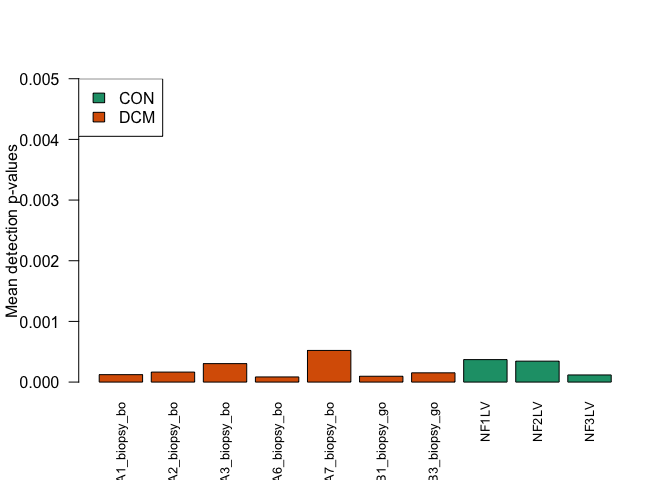
\includegraphics{README_files/figure-latex/EPIC_Import-1.pdf}

\begin{Shaded}
\begin{Highlighting}[]
\CommentTok{\# \#Determine the fraction of "failed" CpG probes (those which failed to identify a methylated CpG)}
\CommentTok{\# colMeans(failed)}
\CommentTok{\#Convert R/G to Methylated/Unmethylated in an object of class MethylSet}
\NormalTok{MSet}\OtherTok{\textless{}{-}}\FunctionTok{preprocessRaw}\NormalTok{(RGSet)}
\CommentTok{\#QC data}
\NormalTok{qc}\OtherTok{\textless{}{-}}\FunctionTok{getQC}\NormalTok{(MSet)}
\FunctionTok{plotQC}\NormalTok{(qc)}
\end{Highlighting}
\end{Shaded}

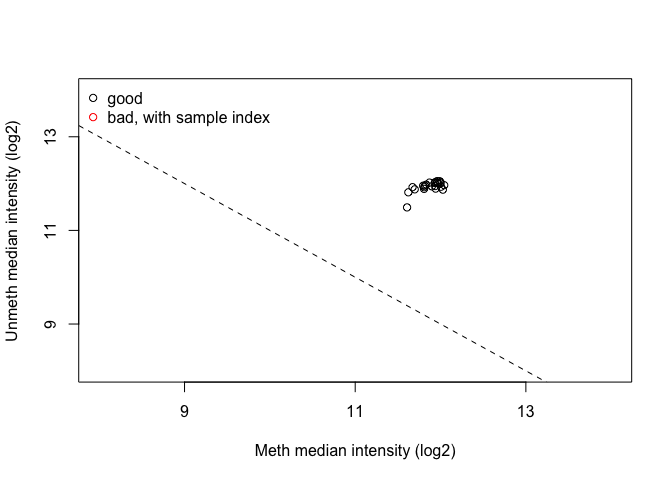
\includegraphics{README_files/figure-latex/EPIC_Import-2.pdf}

\begin{Shaded}
\begin{Highlighting}[]
\FunctionTok{pdf}\NormalTok{(}\AttributeTok{file=}\FunctionTok{paste0}\NormalTok{(}\StringTok{"../2\_Output/"}\NormalTok{, COMPARISON, }\StringTok{"/"}\NormalTok{, COMPARISON, }\StringTok{"\_QC.Methyl.pdf"}\NormalTok{))}
\FunctionTok{plotQC}\NormalTok{(qc)}
\FunctionTok{dev.off}\NormalTok{()}
\end{Highlighting}
\end{Shaded}

\begin{verbatim}
## pdf 
##   2
\end{verbatim}

\begin{Shaded}
\begin{Highlighting}[]
\DocumentationTok{\#\#Density plot}
\CommentTok{\# densityPlot(RGSet, sampGroups = targets$Sample\_Group, main= "Beta", xlab = "Beta")}
\FunctionTok{pdf}\NormalTok{(}\AttributeTok{file=}\FunctionTok{paste0}\NormalTok{(}\StringTok{"../2\_Output/"}\NormalTok{, COMPARISON, }\StringTok{"/"}\NormalTok{, COMPARISON, }\StringTok{"\_densityPlot.pdf"}\NormalTok{))}
\FunctionTok{densityPlot}\NormalTok{(RGSet, }\AttributeTok{sampGroups =}\NormalTok{ targets}\SpecialCharTok{$}\NormalTok{Sample\_Group, }\AttributeTok{main=} \StringTok{"Beta"}\NormalTok{, }\AttributeTok{xlab =} \StringTok{"Beta"}\NormalTok{)}
\FunctionTok{dev.off}\NormalTok{()}
\end{Highlighting}
\end{Shaded}

\begin{verbatim}
## pdf 
##   2
\end{verbatim}

\begin{Shaded}
\begin{Highlighting}[]
\FunctionTok{densityBeanPlot}\NormalTok{(RGSet, }\AttributeTok{sampGroups =}\NormalTok{ targets}\SpecialCharTok{$}\NormalTok{Sample\_Group)}
\end{Highlighting}
\end{Shaded}

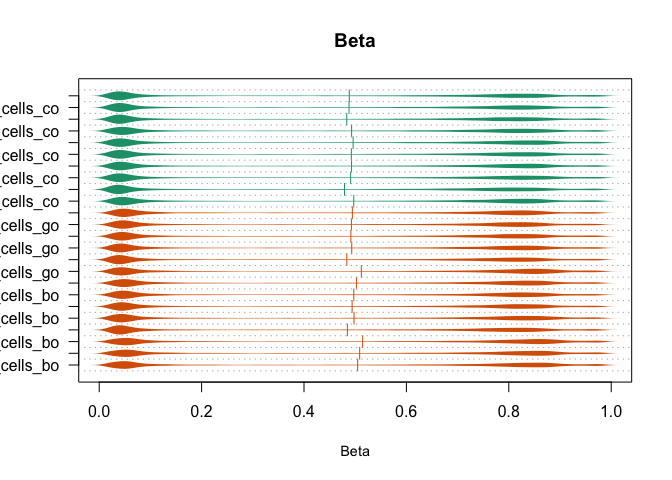
\includegraphics{README_files/figure-latex/EPIC_Import-3.pdf}

\begin{Shaded}
\begin{Highlighting}[]
\FunctionTok{pdf}\NormalTok{(}\AttributeTok{file=}\FunctionTok{paste0}\NormalTok{(}\StringTok{"../2\_Output/"}\NormalTok{, COMPARISON, }\StringTok{"/"}\NormalTok{, COMPARISON, }\StringTok{"\_BeanPlot.pdf"}\NormalTok{))}
\FunctionTok{densityBeanPlot}\NormalTok{(RGSet, }\AttributeTok{sampGroups =}\NormalTok{ targets}\SpecialCharTok{$}\NormalTok{Sample\_Group)}
\FunctionTok{dev.off}\NormalTok{()}
\end{Highlighting}
\end{Shaded}

\begin{verbatim}
## pdf 
##   2
\end{verbatim}

\begin{Shaded}
\begin{Highlighting}[]
\FunctionTok{qcReport}\NormalTok{(RGSet, }\AttributeTok{pdf=} \FunctionTok{paste0}\NormalTok{(}\StringTok{"../2\_Output/"}\NormalTok{, COMPARISON, }\StringTok{"/"}\NormalTok{, COMPARISON, }\StringTok{"\_qcReport.pdf"}\NormalTok{))}
\end{Highlighting}
\end{Shaded}

\begin{verbatim}
## pdf 
##   2
\end{verbatim}

\begin{Shaded}
\begin{Highlighting}[]
\CommentTok{\# \#Convert to a shinyMethyl dataset (nice summary of the quality control)}
\CommentTok{\# summarized.data \textless{}{-} shinySummarize(RGSet)}
\CommentTok{\# runShinyMethyl(summarized.data)}

\NormalTok{gRatioSet.quantile }\OtherTok{\textless{}{-}} \FunctionTok{preprocessQuantile}\NormalTok{(RGSet, }\AttributeTok{fixOutliers =} \ConstantTok{TRUE}\NormalTok{, }\AttributeTok{removeBadSamples =} \ConstantTok{TRUE}\NormalTok{, }\AttributeTok{badSampleCutoff =} \FloatTok{10.5}\NormalTok{, }\AttributeTok{quantileNormalize =} \ConstantTok{TRUE}\NormalTok{, }\AttributeTok{stratified =} \ConstantTok{TRUE}\NormalTok{, }\AttributeTok{mergeManifest =} \ConstantTok{FALSE}\NormalTok{)}
\NormalTok{beta.all}\OtherTok{\textless{}{-}}\FunctionTok{getBeta}\NormalTok{(RGSet)}
\FunctionTok{write.csv}\NormalTok{(beta.all, }\StringTok{"../1\_Input/EPIC.betaValues.csv"}\NormalTok{)}
\end{Highlighting}
\end{Shaded}

\hypertarget{supplemental-figure-sxx-outlier-analysis}{%
\subsection{Supplemental Figure SXX: Outlier
Analysis}\label{supplemental-figure-sxx-outlier-analysis}}

\begin{Shaded}
\begin{Highlighting}[]
\FunctionTok{par}\NormalTok{(}\AttributeTok{mfrow=}\FunctionTok{c}\NormalTok{(}\DecValTok{1}\NormalTok{,}\DecValTok{1}\NormalTok{))}
\FunctionTok{barplot}\NormalTok{(}\FunctionTok{colMeans}\NormalTok{(detP), }\AttributeTok{col=}\NormalTok{PLOT.COL[}\FunctionTok{factor}\NormalTok{(targets}\SpecialCharTok{$}\NormalTok{Sample\_Group)], }\AttributeTok{las=}\DecValTok{2}\NormalTok{, }
        \AttributeTok{cex.names=}\FloatTok{0.8}\NormalTok{, }\AttributeTok{ylim=}\FunctionTok{c}\NormalTok{(}\DecValTok{0}\NormalTok{,}\FloatTok{0.005}\NormalTok{), }\AttributeTok{ylab=}\StringTok{"Mean detection p{-}values"}\NormalTok{)}
\FunctionTok{abline}\NormalTok{(}\AttributeTok{h=}\FloatTok{0.05}\NormalTok{,}\AttributeTok{col=}\StringTok{"red"}\NormalTok{)}
\FunctionTok{legend}\NormalTok{(}\StringTok{"topleft"}\NormalTok{, }\AttributeTok{legend=}\FunctionTok{levels}\NormalTok{(}\FunctionTok{factor}\NormalTok{(targets}\SpecialCharTok{$}\NormalTok{Sample\_Group)), }\AttributeTok{fill=}\NormalTok{PLOT.COL, }
       \AttributeTok{bg=}\StringTok{"white"}\NormalTok{)}
\end{Highlighting}
\end{Shaded}

\begin{figure}
\centering
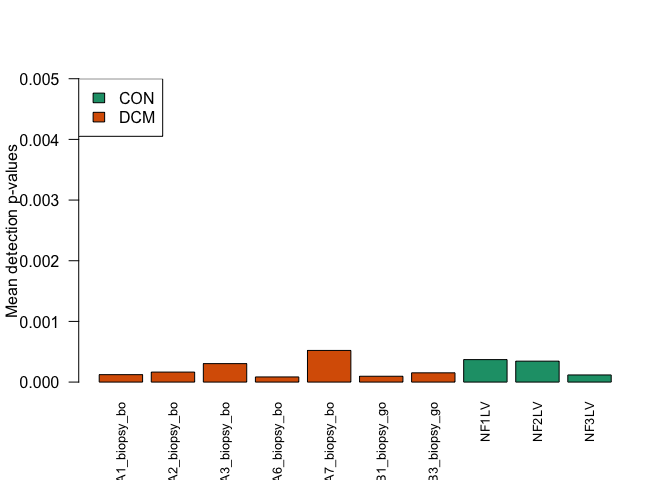
\includegraphics{README_files/figure-latex/outliers-1.pdf}
\caption{Supplemental Figure}
\end{figure}

\hypertarget{figure-2a-mds-plot---unsupervised-clustering-by-sample_group}{%
\subsection{Figure 2A: MDS Plot - Unsupervised Clustering by
``Sample\_Group''}\label{figure-2a-mds-plot---unsupervised-clustering-by-sample_group}}

Because such a robust racial signature in cardiac DNA methylation was
seen in the pilot analysis, we reproduced the unsupervised method in the
larger cohort. This time, we continue to see a distinct racial
difference. Furthermore, we found that this racially-determined
clustering persisted to among the 500,000 most-variable CpG probes in
the EPIC array.

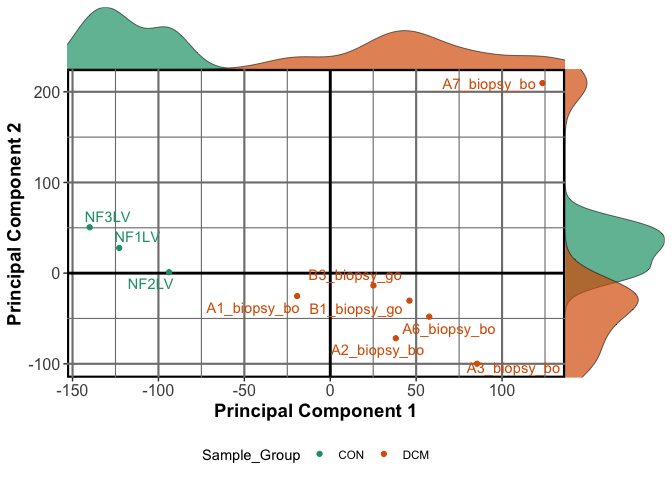
\includegraphics{README_files/figure-latex/MDS.methyl-1.pdf}

\hypertarget{pca}{%
\subsection{PCA}\label{pca}}

\begin{Shaded}
\begin{Highlighting}[]
\CommentTok{\#Plot Features of the PCA}
\FunctionTok{library}\NormalTok{(dplyr)}
\FunctionTok{library}\NormalTok{(plotly)}
\DocumentationTok{\#\#Import the data to be used for PCA}
\NormalTok{Index\_PCA}\OtherTok{\textless{}{-}}\NormalTok{targets}
\FunctionTok{rownames}\NormalTok{(Index\_PCA)}\OtherTok{\textless{}{-}}\NormalTok{Index\_PCA}\SpecialCharTok{$}\NormalTok{Sample\_Name}
\NormalTok{PCA\_data}\OtherTok{\textless{}{-}}\FunctionTok{as.data.frame}\NormalTok{(}\FunctionTok{getM}\NormalTok{(gRatioSet.quantile))}
\CommentTok{\#transpose the dataset (required for PCA)}
\NormalTok{data.pca}\OtherTok{\textless{}{-}}\FunctionTok{t}\NormalTok{(PCA\_data)}
\NormalTok{data.pca}\OtherTok{\textless{}{-}}\FunctionTok{as.data.frame}\NormalTok{(data.pca)}
\DocumentationTok{\#\#merge the file}
\NormalTok{data.pca\_Final}\OtherTok{\textless{}{-}}\FunctionTok{merge}\NormalTok{(Index\_PCA, data.pca, }\AttributeTok{by=}\DecValTok{0}\NormalTok{)}
\FunctionTok{rownames}\NormalTok{(data.pca\_Final)}\OtherTok{\textless{}{-}}\NormalTok{data.pca\_Final}\SpecialCharTok{$}\NormalTok{Row.names}
\NormalTok{pca.comp}\OtherTok{\textless{}{-}}\FunctionTok{prcomp}\NormalTok{(data.pca\_Final[,(}\FunctionTok{ncol}\NormalTok{(Index\_PCA)}\SpecialCharTok{+}\DecValTok{2}\NormalTok{)}\SpecialCharTok{:}\FunctionTok{ncol}\NormalTok{(data.pca\_Final)])}

\NormalTok{pcaCharts}\OtherTok{=}\ControlFlowTok{function}\NormalTok{(x) \{}
\NormalTok{    x.var }\OtherTok{\textless{}{-}}\NormalTok{ x}\SpecialCharTok{$}\NormalTok{sdev }\SpecialCharTok{\^{}} \DecValTok{2}
\NormalTok{    x.pvar }\OtherTok{\textless{}{-}}\NormalTok{ x.var}\SpecialCharTok{/}\FunctionTok{sum}\NormalTok{(x.var)}
    \FunctionTok{par}\NormalTok{(}\AttributeTok{mfrow=}\FunctionTok{c}\NormalTok{(}\DecValTok{2}\NormalTok{,}\DecValTok{2}\NormalTok{))}
    \FunctionTok{plot}\NormalTok{(x.pvar,}\AttributeTok{xlab=}\StringTok{"Principal component"}\NormalTok{,}
         \AttributeTok{ylab=}\StringTok{"Proportion of variance"}\NormalTok{, }\AttributeTok{ylim=}\FunctionTok{c}\NormalTok{(}\DecValTok{0}\NormalTok{,}\DecValTok{1}\NormalTok{), }\AttributeTok{type=}\StringTok{\textquotesingle{}b\textquotesingle{}}\NormalTok{)}
    \FunctionTok{plot}\NormalTok{(}\FunctionTok{cumsum}\NormalTok{(x.pvar),}\AttributeTok{xlab=}\StringTok{"Principal component"}\NormalTok{,}
         \AttributeTok{ylab=}\StringTok{"Cumulative Proportion of variance"}\NormalTok{,}
         \AttributeTok{ylim=}\FunctionTok{c}\NormalTok{(}\DecValTok{0}\NormalTok{,}\DecValTok{1}\NormalTok{),}
         \AttributeTok{type=}\StringTok{\textquotesingle{}b\textquotesingle{}}\NormalTok{)}
    \FunctionTok{screeplot}\NormalTok{(x)}
    \FunctionTok{screeplot}\NormalTok{(x,}\AttributeTok{type=}\StringTok{"l"}\NormalTok{)}
    \FunctionTok{par}\NormalTok{(}\AttributeTok{mfrow=}\FunctionTok{c}\NormalTok{(}\DecValTok{1}\NormalTok{,}\DecValTok{1}\NormalTok{))}
\NormalTok{\}}
\FunctionTok{pcaCharts}\NormalTok{(pca.comp)}
\end{Highlighting}
\end{Shaded}

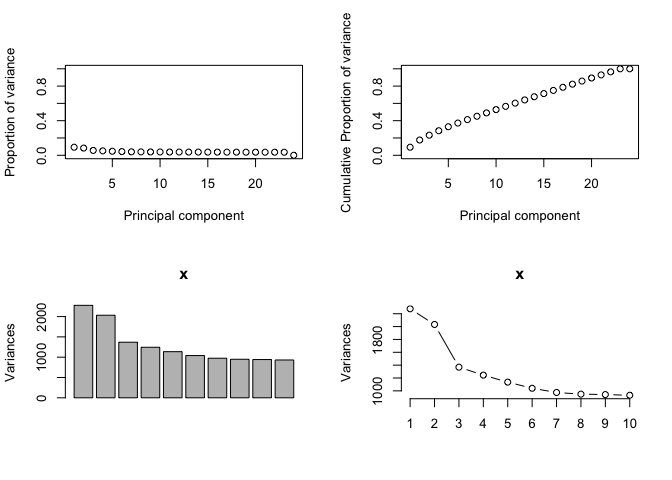
\includegraphics{README_files/figure-latex/PCA_Features-1.pdf}

\begin{Shaded}
\begin{Highlighting}[]
\FunctionTok{png}\NormalTok{(}\AttributeTok{file=}\FunctionTok{paste0}\NormalTok{(}\StringTok{"../2\_Output/"}\NormalTok{, COMPARISON,  }\StringTok{"/"}\NormalTok{, COMPARISON, }\StringTok{"\_PCA.Charts.png"}\NormalTok{))}
\FunctionTok{pcaCharts}\NormalTok{(pca.comp)}
\FunctionTok{dev.off}\NormalTok{()}
\end{Highlighting}
\end{Shaded}

\begin{verbatim}
## pdf 
##   2
\end{verbatim}

\hypertarget{dimensional-pca}{%
\subsubsection{3-Dimensional PCA}\label{dimensional-pca}}

From the previous calculations, it is seens that only 2 principal
components are necessary (accounting for \textgreater80\% cumulative
variance). Nonetheless, below is a 3-D PCA to ensure that all groups are
characterize to higher-degree of stringency. Nevertheless, a racial
difference could not be appreciated.

\begin{Shaded}
\begin{Highlighting}[]
\DocumentationTok{\#\#Create a 3D{-}PCA for Inspection}
\FunctionTok{library}\NormalTok{(plotly)}
\DocumentationTok{\#\#Index}
\NormalTok{Index\_PCA}\OtherTok{\textless{}{-}}\NormalTok{targets}
\FunctionTok{rownames}\NormalTok{(Index\_PCA)}\OtherTok{\textless{}{-}}\NormalTok{Index\_PCA}\SpecialCharTok{$}\NormalTok{Sample\_Name}

\NormalTok{PCs}\OtherTok{\textless{}{-}}\FunctionTok{merge}\NormalTok{(pca.comp}\SpecialCharTok{$}\NormalTok{x, Index\_PCA, }\AttributeTok{by=}\DecValTok{0}\NormalTok{)}
\FunctionTok{rownames}\NormalTok{(PCs)}\OtherTok{\textless{}{-}}\NormalTok{PCs}\SpecialCharTok{$}\NormalTok{Row.names}
\NormalTok{PCs}\SpecialCharTok{$}\NormalTok{Group }\OtherTok{\textless{}{-}} \FunctionTok{as.factor}\NormalTok{(PCs}\SpecialCharTok{$}\NormalTok{Sample\_Group)}
\NormalTok{fig }\OtherTok{\textless{}{-}} \FunctionTok{plot\_ly}\NormalTok{(PCs, }\AttributeTok{x =} \SpecialCharTok{\textasciitilde{}}\NormalTok{PC1, }\AttributeTok{y =} \SpecialCharTok{\textasciitilde{}}\NormalTok{PC2, }\AttributeTok{z =} \SpecialCharTok{\textasciitilde{}}\NormalTok{PC3, }\AttributeTok{color =} \SpecialCharTok{\textasciitilde{}}\NormalTok{Sample\_Group, }\AttributeTok{text =} \SpecialCharTok{\textasciitilde{}}\FunctionTok{paste}\NormalTok{(}\StringTok{\textquotesingle{}Sample\_Name:\textquotesingle{}}\NormalTok{, Sample\_Name, }\StringTok{\textquotesingle{}\textless{}br\textgreater{}Tissue:\textquotesingle{}}\NormalTok{, Tissue, }\StringTok{\textquotesingle{}\textless{}br\textgreater{}Outcome:\textquotesingle{}}\NormalTok{, Outcome, }\StringTok{\textquotesingle{}\textless{}br\textgreater{}Sex:\textquotesingle{}}\NormalTok{, Sex))}
\NormalTok{fig }\OtherTok{\textless{}{-}}\NormalTok{ fig }\SpecialCharTok{\%\textgreater{}\%} \FunctionTok{add\_markers}\NormalTok{()}
\NormalTok{fig }\OtherTok{\textless{}{-}}\NormalTok{ fig }\SpecialCharTok{\%\textgreater{}\%} \FunctionTok{layout}\NormalTok{(}\AttributeTok{scene =} \FunctionTok{list}\NormalTok{(}\AttributeTok{xaxis =} \FunctionTok{list}\NormalTok{(}\AttributeTok{title =} \StringTok{\textquotesingle{}PC1\textquotesingle{}}\NormalTok{),}
                     \AttributeTok{yaxis =} \FunctionTok{list}\NormalTok{(}\AttributeTok{title =} \StringTok{\textquotesingle{}PC2\textquotesingle{}}\NormalTok{),}
                     \AttributeTok{zaxis =} \FunctionTok{list}\NormalTok{(}\AttributeTok{title =} \StringTok{\textquotesingle{}PC3\textquotesingle{}}\NormalTok{)))}
\NormalTok{fig}
\end{Highlighting}
\end{Shaded}

\hypertarget{differential-methylation-of-ipscs-dcm-vs.-con}{%
\subsection{Differential Methylation of iPSCs (DCM
vs.~CON)}\label{differential-methylation-of-ipscs-dcm-vs.-con}}

\hypertarget{using-minfi-to-compute-differential-expression}{%
\subsection{Using Minfi to compute differential
expression}\label{using-minfi-to-compute-differential-expression}}

Owing to the apparent separation by patient Sample\_Group, we chose to
identify the CpG sites responsible for a Sample\_Group-based epigenomic
difference.

\begin{Shaded}
\begin{Highlighting}[]
\CommentTok{\#Quantification and Differential Expression Analysis}
\NormalTok{RGSet}\OtherTok{\textless{}{-}}\FunctionTok{read.metharray.exp}\NormalTok{(}\AttributeTok{base =} \StringTok{"../1\_Input/IDAT"}\NormalTok{, }\AttributeTok{targets =}\NormalTok{ targets, }\AttributeTok{verbose =} \ConstantTok{TRUE}\NormalTok{)}
\CommentTok{\# sampleNames(RGSet)\textless{}{-}targets$Sample\_Name}
\NormalTok{GRset.funnorm }\OtherTok{\textless{}{-}} \FunctionTok{preprocessFunnorm}\NormalTok{(RGSet)}
\NormalTok{beta }\OtherTok{\textless{}{-}} \FunctionTok{getBeta}\NormalTok{(GRset.funnorm)}
\NormalTok{M}\OtherTok{\textless{}{-}}\FunctionTok{getM}\NormalTok{(GRset.funnorm)}
\NormalTok{Condition }\OtherTok{\textless{}{-}} \FunctionTok{pData}\NormalTok{(GRset.funnorm)}\SpecialCharTok{$}\NormalTok{Sample\_Group}
\NormalTok{dmp }\OtherTok{\textless{}{-}} \FunctionTok{dmpFinder}\NormalTok{(beta, }\AttributeTok{pheno =}\NormalTok{ Condition  , }\AttributeTok{type =} \StringTok{"categorical"}\NormalTok{)}
\NormalTok{DMPs}\OtherTok{\textless{}{-}}\FunctionTok{merge}\NormalTok{(dmp, annoM450k, }\AttributeTok{by=} \DecValTok{0}\NormalTok{)}
\NormalTok{DMPs}\OtherTok{\textless{}{-}}\FunctionTok{as.data.frame}\NormalTok{(DMPs)}
\FunctionTok{rownames}\NormalTok{(DMPs)}\OtherTok{\textless{}{-}}\NormalTok{DMPs}\SpecialCharTok{$}\NormalTok{Row.names}
\NormalTok{DMPs}\OtherTok{\textless{}{-}}\NormalTok{DMPs }\SpecialCharTok{\%\textgreater{}\%}\NormalTok{ dplyr}\SpecialCharTok{::}\FunctionTok{select}\NormalTok{(}\SpecialCharTok{{-}}\NormalTok{Row.names)}
\CommentTok{\#create an beta table}
\NormalTok{beta.table}\OtherTok{\textless{}{-}}\FunctionTok{as.data.frame}\NormalTok{(}\FunctionTok{t}\NormalTok{(beta))}
\NormalTok{beta.table}\SpecialCharTok{$}\NormalTok{Col\_ID}\OtherTok{\textless{}{-}}\FunctionTok{rownames}\NormalTok{(beta.table)}
\NormalTok{beta\_named}\OtherTok{\textless{}{-}}\FunctionTok{merge}\NormalTok{(beta.table, targets, }\AttributeTok{by =} \StringTok{"Col\_ID"}\NormalTok{)}
\FunctionTok{rownames}\NormalTok{(beta\_named)}\OtherTok{\textless{}{-}}\NormalTok{beta\_named}\SpecialCharTok{$}\NormalTok{Sample\_Name}
\NormalTok{beta\_named}\OtherTok{\textless{}{-}}\NormalTok{beta\_named }\SpecialCharTok{\%\textgreater{}\%}\NormalTok{ dplyr}\SpecialCharTok{::}\FunctionTok{select}\NormalTok{(}\SpecialCharTok{{-}}\FunctionTok{names}\NormalTok{(targets)) }\SpecialCharTok{\%\textgreater{}\%} \FunctionTok{t}\NormalTok{()}
\FunctionTok{write.csv}\NormalTok{(beta\_named, }\FunctionTok{paste0}\NormalTok{(}\StringTok{"../2\_Output/"}\NormalTok{, COMPARISON, }\StringTok{"/"}\NormalTok{, COMPARISON, }\StringTok{"\_beta.table.csv"}\NormalTok{))}
\CommentTok{\#Add beta values to statistics}
\NormalTok{Results\_dmp}\OtherTok{\textless{}{-}}\FunctionTok{merge}\NormalTok{(DMPs, beta\_named, }\AttributeTok{by =} \DecValTok{0}\NormalTok{)}
\CommentTok{\#Calculate Average CpG Methylation by Sample\_Group}
\FunctionTok{library}\NormalTok{(dplyr)}
\FunctionTok{library}\NormalTok{(matrixStats)}
\NormalTok{Results}\OtherTok{\textless{}{-}}\NormalTok{Results\_dmp }\SpecialCharTok{\%\textgreater{}\%} \FunctionTok{replace}\NormalTok{(}\FunctionTok{is.na}\NormalTok{(.), }\DecValTok{0}\NormalTok{) }\SpecialCharTok{\%\textgreater{}\%}\NormalTok{ dplyr}\SpecialCharTok{::}\FunctionTok{mutate}\NormalTok{(}
  \AttributeTok{DCM\_SD =} \FunctionTok{rowSds}\NormalTok{(}\FunctionTok{as.matrix}\NormalTok{(Results\_dmp[,targets}\SpecialCharTok{$}\NormalTok{Sample\_Name[targets}\SpecialCharTok{$}\NormalTok{Sample\_Group}\SpecialCharTok{==}\StringTok{"DCM"}\NormalTok{]])),}
  \AttributeTok{DCM\_Mean =} \FunctionTok{rowMeans}\NormalTok{(}\FunctionTok{as.matrix}\NormalTok{(Results\_dmp[,targets}\SpecialCharTok{$}\NormalTok{Sample\_Name[targets}\SpecialCharTok{$}\NormalTok{Sample\_Group}\SpecialCharTok{==}\StringTok{"DCM"}\NormalTok{]])),}
  \AttributeTok{CON\_SD =} \FunctionTok{rowSds}\NormalTok{(}\FunctionTok{as.matrix}\NormalTok{(Results\_dmp[,targets}\SpecialCharTok{$}\NormalTok{Sample\_Name[targets}\SpecialCharTok{$}\NormalTok{Sample\_Group}\SpecialCharTok{==}\StringTok{"CON"}\NormalTok{]])),}
  \AttributeTok{CON\_Mean =} \FunctionTok{rowMeans}\NormalTok{(}\FunctionTok{as.matrix}\NormalTok{(Results\_dmp[,targets}\SpecialCharTok{$}\NormalTok{Sample\_Name[targets}\SpecialCharTok{$}\NormalTok{Sample\_Group}\SpecialCharTok{==}\StringTok{"CON"}\NormalTok{]])),}
  \AttributeTok{Methylation.Diff=}\NormalTok{(DCM\_Mean}\SpecialCharTok{{-}}\NormalTok{CON\_Mean)}\SpecialCharTok{*}\DecValTok{100}\NormalTok{)}
\FunctionTok{rownames}\NormalTok{(Results)}\OtherTok{\textless{}{-}}\NormalTok{Results}\SpecialCharTok{$}\NormalTok{Row.names}
\NormalTok{Results\_dmp\_p05}\OtherTok{\textless{}{-}}\FunctionTok{filter}\NormalTok{(Results, pval}\SpecialCharTok{\textless{}}\FloatTok{0.05}\NormalTok{)}
\NormalTok{Results\_dmp\_q05}\OtherTok{\textless{}{-}}\FunctionTok{filter}\NormalTok{(Results, qval}\SpecialCharTok{\textless{}}\FloatTok{0.05}\NormalTok{)}
\DocumentationTok{\#\#\#\#\#\#\#\#\#\#\#\#\#\#\#\#\#\#\#\#\#\#\#\#\#\#\#\#\#\#\#\#\#\#\#\#\#\#\#\#\#}
\CommentTok{\#Identify Promoter{-}associated CpG Islands}
\FunctionTok{library}\NormalTok{(tidyr)}
\NormalTok{PromCGI}\OtherTok{\textless{}{-}}\NormalTok{dplyr}\SpecialCharTok{::}\FunctionTok{filter}\NormalTok{(Results\_dmp\_p05, }\FunctionTok{grepl}\NormalTok{(}\StringTok{"Island"}\NormalTok{, Relation\_to\_Island), }\FunctionTok{grepl}\NormalTok{(}\StringTok{"TSS"}\NormalTok{, UCSC\_RefGene\_Group))}
\CommentTok{\#Separate Gene Names into unique rows}
\NormalTok{PromCGI\_sep}\OtherTok{\textless{}{-}}\NormalTok{PromCGI }\SpecialCharTok{\%\textgreater{}\%} \FunctionTok{mutate}\NormalTok{(}\AttributeTok{UCSC\_RefGene\_Name =} \FunctionTok{strsplit}\NormalTok{(}\FunctionTok{as.character}\NormalTok{(UCSC\_RefGene\_Name), }\StringTok{";"}\NormalTok{)) }\SpecialCharTok{\%\textgreater{}\%} \FunctionTok{unnest}\NormalTok{(UCSC\_RefGene\_Name) }\SpecialCharTok{\%\textgreater{}\%} \FunctionTok{distinct}\NormalTok{()}
\CommentTok{\#Save a copy of the countData}
\FunctionTok{library}\NormalTok{(openxlsx)}
\NormalTok{wb\_countData}\OtherTok{\textless{}{-}}\FunctionTok{createWorkbook}\NormalTok{()}
\FunctionTok{addWorksheet}\NormalTok{(wb\_countData, }\StringTok{"Unfiltered"}\NormalTok{)}
  \FunctionTok{writeData}\NormalTok{(wb\_countData, }\StringTok{"Unfiltered"}\NormalTok{, Results, }\AttributeTok{startCol =} \DecValTok{1}\NormalTok{)}
\FunctionTok{addWorksheet}\NormalTok{(wb\_countData, }\StringTok{"P\_0.05"}\NormalTok{)}
  \FunctionTok{writeData}\NormalTok{(wb\_countData, }\StringTok{"P\_0.05"}\NormalTok{, Results\_dmp\_p05, }\AttributeTok{startCol =} \DecValTok{1}\NormalTok{)}
\FunctionTok{addWorksheet}\NormalTok{(wb\_countData, }\StringTok{"Q\_0.05"}\NormalTok{)}
  \FunctionTok{writeData}\NormalTok{(wb\_countData, }\StringTok{"Q\_0.05"}\NormalTok{, Results\_dmp\_q05, }\AttributeTok{startCol =} \DecValTok{1}\NormalTok{)}
\FunctionTok{addWorksheet}\NormalTok{(wb\_countData, }\StringTok{"Promoter.CGI"}\NormalTok{)}
  \FunctionTok{writeData}\NormalTok{(wb\_countData, }\StringTok{"Promoter.CGI"}\NormalTok{, PromCGI\_sep, }\AttributeTok{startCol =} \DecValTok{1}\NormalTok{)}
\FunctionTok{saveWorkbook}\NormalTok{(wb\_countData, }\AttributeTok{file =} \FunctionTok{paste0}\NormalTok{(}\StringTok{"../2\_Output/"}\NormalTok{, COMPARISON, }\StringTok{"/"}\NormalTok{, COMPARISON, }\StringTok{"\_DMPs.xlsx"}\NormalTok{), }\AttributeTok{overwrite =} \ConstantTok{TRUE}\NormalTok{)}
\end{Highlighting}
\end{Shaded}

\hypertarget{distribution-of-methylation-by-genomic-and-cpg-annotation}{%
\subsection{Distribution of Methylation by Genomic and CpG
Annotation}\label{distribution-of-methylation-by-genomic-and-cpg-annotation}}

The following figure illustrates the enrichment of differential
methylation with respect to CpG-based and genomic annotations.

\begin{Shaded}
\begin{Highlighting}[]
\FunctionTok{library}\NormalTok{(plotly)}
\FunctionTok{library}\NormalTok{(dplyr)}
\FunctionTok{library}\NormalTok{(tidyr)}
\FunctionTok{library}\NormalTok{(stringr)}
\FunctionTok{library}\NormalTok{(reshape2)}
\FunctionTok{library}\NormalTok{(readxl)}
\FunctionTok{library}\NormalTok{(kableExtra)}
\FunctionTok{library}\NormalTok{(ComplexHeatmap)}
\FunctionTok{library}\NormalTok{(openxlsx)}

\DocumentationTok{\#\#Create a regional annotation matrix of the m450k array}
\NormalTok{Region\_epic}\OtherTok{\textless{}{-}}\NormalTok{Results\_dmp }\SpecialCharTok{\%\textgreater{}\%} 
\NormalTok{  dplyr}\SpecialCharTok{::}\FunctionTok{select}\NormalTok{(Row.names, UCSC\_RefGene\_Group, Relation\_to\_Island)}
\NormalTok{Stage1}\OtherTok{\textless{}{-}}\NormalTok{Region\_epic }\SpecialCharTok{\%\textgreater{}\%} 
  \FunctionTok{mutate}\NormalTok{(}\AttributeTok{UCSC\_RefGene\_Group =} \FunctionTok{strsplit}\NormalTok{(}\FunctionTok{as.character}\NormalTok{(UCSC\_RefGene\_Group), }\StringTok{";"}\NormalTok{)) }\SpecialCharTok{\%\textgreater{}\%} 
  \FunctionTok{unnest}\NormalTok{(UCSC\_RefGene\_Group) }
\NormalTok{Stage2}\OtherTok{\textless{}{-}}\NormalTok{Stage1 }\SpecialCharTok{\%\textgreater{}\%} 
  \FunctionTok{mutate}\NormalTok{(}\AttributeTok{Relation\_to\_Island =} \FunctionTok{strsplit}\NormalTok{(}\FunctionTok{as.character}\NormalTok{(Relation\_to\_Island), }\StringTok{";"}\NormalTok{)) }\SpecialCharTok{\%\textgreater{}\%}  
  \FunctionTok{unnest}\NormalTok{(Relation\_to\_Island)}
\NormalTok{Stage3}\OtherTok{\textless{}{-}}\FunctionTok{distinct}\NormalTok{(Stage2)}
\NormalTok{Regional.Groups}\OtherTok{\textless{}{-}}\NormalTok{dplyr}\SpecialCharTok{::}\FunctionTok{group\_by\_}\NormalTok{(Stage3, }\StringTok{"UCSC\_RefGene\_Group"}\NormalTok{, }\StringTok{"Relation\_to\_Island"}\NormalTok{) }\SpecialCharTok{\%\textgreater{}\%} 
  \FunctionTok{tally}\NormalTok{()}
\NormalTok{Region.matrix}\OtherTok{\textless{}{-}}\NormalTok{Regional.Groups }\SpecialCharTok{\%\textgreater{}\%} 
  \FunctionTok{spread}\NormalTok{(Relation\_to\_Island, n)}
\NormalTok{Region.matrix}\OtherTok{\textless{}{-}}\NormalTok{Region.matrix }\SpecialCharTok{\%\textgreater{}\%} 
\NormalTok{  dplyr}\SpecialCharTok{::}\FunctionTok{select}\NormalTok{(UCSC\_RefGene\_Group, OpenSea, N\_Shelf, N\_Shore, Island, S\_Shore, S\_Shelf)}
\FunctionTok{rownames}\NormalTok{(Region.matrix)}\OtherTok{\textless{}{-}}\NormalTok{Region.matrix}\SpecialCharTok{$}\NormalTok{UCSC\_RefGene\_Group}
\NormalTok{Region.matrix}\OtherTok{\textless{}{-}}\NormalTok{Region.matrix[}\FunctionTok{c}\NormalTok{(}\StringTok{"TSS1500"}\NormalTok{, }\StringTok{"TSS200"}\NormalTok{, }\StringTok{"5\textquotesingle{}UTR"}\NormalTok{, }\StringTok{"1stExon"}\NormalTok{, }\StringTok{"Body"}\NormalTok{, }\StringTok{"3\textquotesingle{}UTR"}\NormalTok{),]}
\FunctionTok{rownames}\NormalTok{(Region.matrix)}\OtherTok{\textless{}{-}}\NormalTok{Region.matrix}\SpecialCharTok{$}\NormalTok{UCSC\_RefGene\_Group}
\NormalTok{Contour\_3D\_epic}\OtherTok{\textless{}{-}}\NormalTok{Region.matrix[,}\SpecialCharTok{{-}}\DecValTok{1}\NormalTok{]}
\FunctionTok{rownames}\NormalTok{(Contour\_3D\_epic)}\OtherTok{\textless{}{-}}\NormalTok{Region.matrix}\SpecialCharTok{$}\NormalTok{UCSC\_RefGene\_Group}
\FunctionTok{write.xlsx}\NormalTok{(Contour\_3D\_epic, }\StringTok{"../2\_Output/Contour.3D\_EPIC.xlsx"}\NormalTok{, }\AttributeTok{overwrite =} \ConstantTok{TRUE}\NormalTok{)}

\DocumentationTok{\#\#Create a regional annotation matrix of differentially{-}methylated positions}
\NormalTok{Region\_p05}\OtherTok{\textless{}{-}}\NormalTok{Results\_dmp\_p05 }\SpecialCharTok{\%\textgreater{}\%}\NormalTok{ dplyr}\SpecialCharTok{::}\FunctionTok{select}\NormalTok{(Row.names, UCSC\_RefGene\_Group, Relation\_to\_Island)}
\NormalTok{Stage1}\OtherTok{\textless{}{-}}\NormalTok{Region\_p05 }\SpecialCharTok{\%\textgreater{}\%} \FunctionTok{mutate}\NormalTok{(}\AttributeTok{UCSC\_RefGene\_Group =} \FunctionTok{strsplit}\NormalTok{(}\FunctionTok{as.character}\NormalTok{(UCSC\_RefGene\_Group), }\StringTok{";"}\NormalTok{)) }\SpecialCharTok{\%\textgreater{}\%} \FunctionTok{unnest}\NormalTok{(UCSC\_RefGene\_Group) }
\NormalTok{Stage2}\OtherTok{\textless{}{-}}\NormalTok{Stage1 }\SpecialCharTok{\%\textgreater{}\%} \FunctionTok{mutate}\NormalTok{(}\AttributeTok{Relation\_to\_Island =} \FunctionTok{strsplit}\NormalTok{(}\FunctionTok{as.character}\NormalTok{(Relation\_to\_Island), }\StringTok{";"}\NormalTok{)) }\SpecialCharTok{\%\textgreater{}\%}  \FunctionTok{unnest}\NormalTok{(Relation\_to\_Island)}
\NormalTok{Stage3}\OtherTok{\textless{}{-}}\FunctionTok{distinct}\NormalTok{(Stage2)}
\NormalTok{Regional.Groups}\OtherTok{\textless{}{-}}\NormalTok{dplyr}\SpecialCharTok{::}\FunctionTok{group\_by\_}\NormalTok{(Stage3, }\StringTok{"UCSC\_RefGene\_Group"}\NormalTok{, }\StringTok{"Relation\_to\_Island"}\NormalTok{) }\SpecialCharTok{\%\textgreater{}\%} \FunctionTok{tally}\NormalTok{()}
\NormalTok{Region.matrix}\OtherTok{\textless{}{-}}\NormalTok{Regional.Groups }\SpecialCharTok{\%\textgreater{}\%} \FunctionTok{spread}\NormalTok{(Relation\_to\_Island, n)}
\NormalTok{Region.matrix}\OtherTok{\textless{}{-}}\NormalTok{Region.matrix }\SpecialCharTok{\%\textgreater{}\%}\NormalTok{ dplyr}\SpecialCharTok{::}\FunctionTok{select}\NormalTok{(UCSC\_RefGene\_Group, OpenSea, N\_Shelf, N\_Shore, Island, S\_Shore, S\_Shelf)}
\FunctionTok{rownames}\NormalTok{(Region.matrix)}\OtherTok{\textless{}{-}}\NormalTok{Region.matrix}\SpecialCharTok{$}\NormalTok{UCSC\_RefGene\_Group}
\NormalTok{Region.matrix}\OtherTok{\textless{}{-}}\NormalTok{Region.matrix[}\FunctionTok{c}\NormalTok{(}\StringTok{"TSS1500"}\NormalTok{, }\StringTok{"TSS200"}\NormalTok{, }\StringTok{"5\textquotesingle{}UTR"}\NormalTok{, }\StringTok{"1stExon"}\NormalTok{, }\StringTok{"Body"}\NormalTok{, }\StringTok{"3\textquotesingle{}UTR"}\NormalTok{),]}
\FunctionTok{rownames}\NormalTok{(Region.matrix)}\OtherTok{\textless{}{-}}\NormalTok{Region.matrix}\SpecialCharTok{$}\NormalTok{UCSC\_RefGene\_Group}
\NormalTok{Contour\_3D}\OtherTok{\textless{}{-}}\NormalTok{Region.matrix[,}\SpecialCharTok{{-}}\DecValTok{1}\NormalTok{]}
\FunctionTok{rownames}\NormalTok{(Contour\_3D)}\OtherTok{\textless{}{-}}\NormalTok{Region.matrix}\SpecialCharTok{$}\NormalTok{UCSC\_RefGene\_Group}
\FunctionTok{write.csv}\NormalTok{(Contour\_3D, }\StringTok{"../2\_Output/Contour.3D\_DMPs.p05.csv"}\NormalTok{)}
\DocumentationTok{\#\#\# Identify DMP Enrichment (IMPORTANT)}
\NormalTok{Enrichment\_Region}\OtherTok{\textless{}{-}}\NormalTok{Contour\_3D}\SpecialCharTok{/}\NormalTok{Contour\_3D\_epic}
\NormalTok{Promoter\_enr}\OtherTok{\textless{}{-}}\NormalTok{Enrichment\_Region[}\FunctionTok{rownames}\NormalTok{(Enrichment\_Region)}\SpecialCharTok{==}\StringTok{"TSS200"}\NormalTok{,] }\SpecialCharTok{+}\NormalTok{ Enrichment\_Region[}\FunctionTok{rownames}\NormalTok{(Enrichment\_Region)}\SpecialCharTok{==}\StringTok{"TSS1500"}\NormalTok{,]}
\FunctionTok{rownames}\NormalTok{(Promoter\_enr)}\OtherTok{\textless{}{-}}\StringTok{"Promoter"}
\NormalTok{Enrichment\_Region}\OtherTok{\textless{}{-}}\NormalTok{Enrichment\_Region }\SpecialCharTok{\%\textgreater{}\%} 
  \FunctionTok{filter}\NormalTok{(}\SpecialCharTok{!}\FunctionTok{grepl}\NormalTok{(}\StringTok{"TSS"}\NormalTok{, }\FunctionTok{rownames}\NormalTok{(Enrichment\_Region))) }\SpecialCharTok{\%\textgreater{}\%}
  \FunctionTok{rbind}\NormalTok{(Promoter\_enr, .) }\SpecialCharTok{\%\textgreater{}\%}
  \FunctionTok{data.matrix}\NormalTok{()}
\NormalTok{paletteLength}\OtherTok{\textless{}{-}}\DecValTok{100}
\NormalTok{myColor }\OtherTok{\textless{}{-}} \FunctionTok{colorRampPalette}\NormalTok{(}\FunctionTok{c}\NormalTok{(}\StringTok{"dodgerblue4"}\NormalTok{, }\StringTok{"white"}\NormalTok{, }\StringTok{"brown4"}\NormalTok{))(paletteLength)}
\FunctionTok{pheatmap}\NormalTok{(Enrichment\_Region, }\AttributeTok{color =}\NormalTok{ myColor, }\AttributeTok{cluster\_rows =} \ConstantTok{FALSE}\NormalTok{, }\AttributeTok{cluster\_cols =} \ConstantTok{FALSE}\NormalTok{, }\AttributeTok{filename =} \FunctionTok{paste0}\NormalTok{(}\StringTok{"../2\_Output/"}\NormalTok{, COMPARISON, }\StringTok{"/"}\NormalTok{, COMPARISON, }\StringTok{"\_DMP.Distribution.pdf"}\NormalTok{))}
\end{Highlighting}
\end{Shaded}

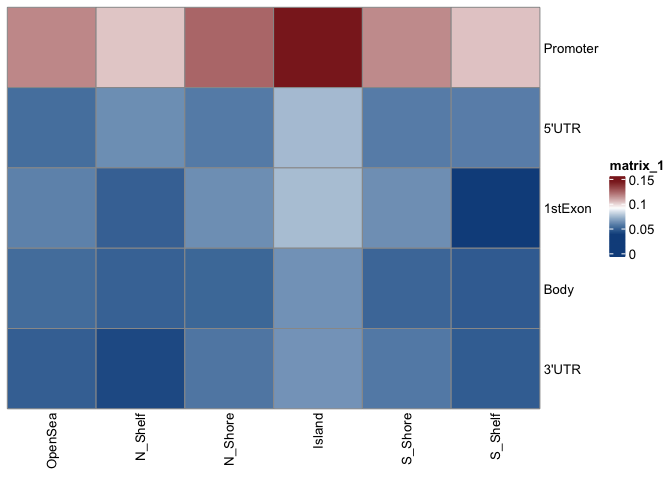
\includegraphics{README_files/figure-latex/Methylation Distribution-1.pdf}

\begin{Shaded}
\begin{Highlighting}[]
\FunctionTok{write.csv}\NormalTok{(Enrichment\_Region, }\StringTok{"DCM\_vs\_CON.csv"}\NormalTok{)}
\DocumentationTok{\#\#Make a Table of the CpG Methylation Distribution}
\NormalTok{Enrichment\_Region }\SpecialCharTok{\%\textgreater{}\%} \FunctionTok{kable}\NormalTok{( }\AttributeTok{align=}\StringTok{"c"}\NormalTok{, }\AttributeTok{booktabs=}\NormalTok{T, }
                     \AttributeTok{caption=}\StringTok{"Methylation Distribution"}\NormalTok{) }\SpecialCharTok{\%\textgreater{}\%} 
  \FunctionTok{kable\_styling}\NormalTok{(}\AttributeTok{latex\_options=}\FunctionTok{c}\NormalTok{(}\StringTok{"striped"}\NormalTok{, }\StringTok{"condensed"}\NormalTok{, }\StringTok{"repeat\_header"}\NormalTok{))}
\end{Highlighting}
\end{Shaded}

\begin{table}

\caption{\label{tab:Methylation Distribution}Methylation Distribution}
\centering
\begin{tabular}[t]{lcccccc}
\toprule
  & OpenSea & N\_Shelf & N\_Shore & Island & S\_Shore & S\_Shelf\\
\midrule
\cellcolor{gray!6}{Promoter} & \cellcolor{gray!6}{0.1164621} & \cellcolor{gray!6}{0.1029990} & \cellcolor{gray!6}{0.1242210} & \cellcolor{gray!6}{0.1460420} & \cellcolor{gray!6}{0.1156378} & \cellcolor{gray!6}{0.1037933}\\
5'UTR & 0.0530359 & 0.0622389 & 0.0569429 & 0.0741839 & 0.0573959 & 0.0576832\\
\cellcolor{gray!6}{1stExon} & \cellcolor{gray!6}{0.0588488} & \cellcolor{gray!6}{0.0489130} & \cellcolor{gray!6}{0.0623833} & \cellcolor{gray!6}{0.0746424} & \cellcolor{gray!6}{0.0625000} & \cellcolor{gray!6}{0.0370370}\\
Body & 0.0523911 & 0.0493794 & 0.0510093 & 0.0633285 & 0.0507863 & 0.0473963\\
\cellcolor{gray!6}{3'UTR} & \cellcolor{gray!6}{0.0485610} & \cellcolor{gray!6}{0.0415879} & \cellcolor{gray!6}{0.0554833} & \cellcolor{gray!6}{0.0638298} & \cellcolor{gray!6}{0.0563931} & \cellcolor{gray!6}{0.0479303}\\
\bottomrule
\end{tabular}
\end{table}

\begin{Shaded}
\begin{Highlighting}[]
\FunctionTok{write.xlsx}\NormalTok{(Enrichment\_Region, }\FunctionTok{paste0}\NormalTok{(}\StringTok{"../2\_Output/"}\NormalTok{, COMPARISON, }\StringTok{"/"}\NormalTok{, COMPARISON, }\StringTok{"\_DMP.Enrichment\_3D.xlsx"}\NormalTok{), }\AttributeTok{overwrite =}\NormalTok{ T)}
\NormalTok{color }\OtherTok{\textless{}{-}} \FunctionTok{colorRampPalette}\NormalTok{(}\FunctionTok{c}\NormalTok{(}\StringTok{"grey"}\NormalTok{, }\StringTok{"orange"}\NormalTok{, }\StringTok{"red"}\NormalTok{))}
\NormalTok{t }\OtherTok{\textless{}{-}} \FunctionTok{list}\NormalTok{(}
  \AttributeTok{family =} \StringTok{"times"}\NormalTok{,}
  \AttributeTok{size =} \DecValTok{16}\NormalTok{,}
  \AttributeTok{color =} \StringTok{"black"}\NormalTok{)}
\NormalTok{x\_axis}\OtherTok{\textless{}{-}}\FunctionTok{list}\NormalTok{(}\AttributeTok{title =} \StringTok{\textquotesingle{}CpG Region\textquotesingle{}}\NormalTok{, }
                     \AttributeTok{type=}\StringTok{"category"}\NormalTok{, }
                     \AttributeTok{zeroline=}\ConstantTok{TRUE}\NormalTok{, }
                     \AttributeTok{showline=}\ConstantTok{TRUE}\NormalTok{, }
                     \AttributeTok{zerolinewidth =} \DecValTok{4}\NormalTok{, }
            \AttributeTok{zerolinecolor=}\StringTok{"darkgrey"}\NormalTok{, }
            \AttributeTok{linecolor=}\StringTok{"darkgrey"}\NormalTok{, }
            \AttributeTok{linewidth=}\DecValTok{4}\NormalTok{, }
            \AttributeTok{titlefont=}\NormalTok{t, }
            \AttributeTok{tickfont=}\NormalTok{t)}
\NormalTok{y\_axis}\OtherTok{\textless{}{-}}\FunctionTok{list}\NormalTok{(}\AttributeTok{title =} \StringTok{\textquotesingle{}Gene Region\textquotesingle{}}\NormalTok{, }
                     \AttributeTok{type=}\StringTok{"category"}\NormalTok{, }
                     \AttributeTok{zeroline=}\ConstantTok{TRUE}\NormalTok{, }
                     \AttributeTok{showline=}\ConstantTok{TRUE}\NormalTok{, }
                     \AttributeTok{zerolinewidth =} \DecValTok{4}\NormalTok{, }
            \AttributeTok{zerolinecolor=}\StringTok{"darkgrey"}\NormalTok{, }
            \AttributeTok{linecolor=}\StringTok{"darkgrey"}\NormalTok{, }
            \AttributeTok{linewidth=}\DecValTok{4}\NormalTok{, }
            \AttributeTok{titlefont=}\NormalTok{t, }
            \AttributeTok{tickfont=}\NormalTok{t)}
\NormalTok{z\_axis}\OtherTok{\textless{}{-}}\FunctionTok{list}\NormalTok{(}\AttributeTok{title =} \StringTok{\textquotesingle{}Number of DMPs\textquotesingle{}}\NormalTok{, }
                     \AttributeTok{zerolinewidth =} \DecValTok{4}\NormalTok{, }
                    \AttributeTok{zerolinecolor=}\StringTok{"darkgrey"}\NormalTok{, }
                    \AttributeTok{linecolor=}\StringTok{"darkgrey"}\NormalTok{, }
                    \AttributeTok{linewidth=}\DecValTok{4}\NormalTok{, }
                    \AttributeTok{titlefont=}\NormalTok{t, }
                    \AttributeTok{tickfont=}\NormalTok{t)}
\NormalTok{q}\OtherTok{\textless{}{-}}\FunctionTok{plot\_ly}\NormalTok{(}\AttributeTok{z=}\SpecialCharTok{\textasciitilde{}}\NormalTok{Enrichment\_Region, }\AttributeTok{colors=}\FunctionTok{color}\NormalTok{(}\DecValTok{10}\NormalTok{), }
    \AttributeTok{text=}\FunctionTok{as.character}\NormalTok{(}\FunctionTok{rownames}\NormalTok{(Enrichment\_Region))) }\SpecialCharTok{\%\textgreater{}\%} \FunctionTok{add\_surface}\NormalTok{() }\SpecialCharTok{\%\textgreater{}\%} 
    \FunctionTok{layout}\NormalTok{(}\AttributeTok{scene =} \FunctionTok{list}\NormalTok{(}\AttributeTok{xaxis =}\NormalTok{ x\_axis, }\AttributeTok{yaxis =}\NormalTok{ y\_axis, }\AttributeTok{zaxis =}\NormalTok{ z\_axis))}
\NormalTok{q }\CommentTok{\#must comment out for PDF generation via knitr (Pandoc).}
\end{Highlighting}
\end{Shaded}

\hypertarget{figure-xx-heatmap-and-hierarchical-clustering-of-differential-methylation-p-0.05}{%
\subsection{Figure XX: Heatmap and Hierarchical Clustering of
Differential Methylation (P \textless{}
0.05)}\label{figure-xx-heatmap-and-hierarchical-clustering-of-differential-methylation-p-0.05}}

Due to the prominent signature of CpG Island-associated promoter
methylation in iPSCs exposed to serum for failing and non-failing
patients, we examined all DMPs present within this region via heatmap.

\begin{Shaded}
\begin{Highlighting}[]
\FunctionTok{library}\NormalTok{(ComplexHeatmap)}
\FunctionTok{library}\NormalTok{(dplyr)}
\DocumentationTok{\#\#Import Data Matrix}
\CommentTok{\# betaHM\textless{}{-}read.csv("../1\_Input/EPIC.betaValues.csv", row.names = 1)}
\DocumentationTok{\#\# Filters to Apply to DMP}
\NormalTok{pvalue\_threshold}\OtherTok{=}\FloatTok{0.001}
\NormalTok{METHYLATION}\OtherTok{=}\DecValTok{0}
\NormalTok{DMP\_location}\OtherTok{=}\StringTok{"Island"}
\NormalTok{Gene\_region}\OtherTok{=}\StringTok{"TSS"}
\NormalTok{Samples}\OtherTok{\textless{}{-}}\NormalTok{AnnoTargets}\SpecialCharTok{$}\NormalTok{Sample\_Name}
\DocumentationTok{\#\#Filter Differential Methylation Data}
\NormalTok{DMP.p05}\OtherTok{\textless{}{-}}\NormalTok{Results }\SpecialCharTok{\%\textgreater{}\%} \FunctionTok{filter}\NormalTok{(pval}\SpecialCharTok{\textless{}}\NormalTok{pvalue\_threshold)}
\NormalTok{DMP.p05}\OtherTok{\textless{}{-}}\NormalTok{DMP.p05 }\SpecialCharTok{\%\textgreater{}\%}\NormalTok{ dplyr}\SpecialCharTok{::}\FunctionTok{select}\NormalTok{(Row.names, }
\NormalTok{                            Methylation.Diff, }
\NormalTok{                            pval, }
\NormalTok{                            qval, }
\NormalTok{                            Relation\_to\_Island, }
\NormalTok{                            UCSC\_RefGene\_Group, }
\NormalTok{                            chr, }
\NormalTok{                            pos, }
                            \FunctionTok{matches}\NormalTok{(Samples)) }\SpecialCharTok{\%\textgreater{}\%}
                      \FunctionTok{filter}\NormalTok{(}\FunctionTok{abs}\NormalTok{(Methylation.Diff)}\SpecialCharTok{\textgreater{}}\NormalTok{METHYLATION)}
\NormalTok{DMP.p05.Region}\OtherTok{\textless{}{-}}\NormalTok{DMP.p05 }\SpecialCharTok{\%\textgreater{}\%} 
  \CommentTok{\# filter(grepl(DMP\_location, Relation\_to\_Island)) \%\textgreater{}\%}
  \FunctionTok{filter}\NormalTok{(}\FunctionTok{grepl}\NormalTok{(Gene\_region, UCSC\_RefGene\_Group)) }\SpecialCharTok{\%\textgreater{}\%} 
\NormalTok{  dplyr}\SpecialCharTok{::}\FunctionTok{select}\NormalTok{(}\FunctionTok{matches}\NormalTok{(AnnoTargets}\SpecialCharTok{$}\NormalTok{Sample\_Name)) }\SpecialCharTok{\%\textgreater{}\%}
  \FunctionTok{data.matrix}\NormalTok{()}
\CommentTok{\#Import the Index File}
\NormalTok{LVAD\_Counts\_Data }\OtherTok{\textless{}{-}}\NormalTok{ targets}
\FunctionTok{rownames}\NormalTok{(LVAD\_Counts\_Data)}\OtherTok{\textless{}{-}}\NormalTok{targets}\SpecialCharTok{$}\NormalTok{Sample\_Name}
\NormalTok{Index}\OtherTok{\textless{}{-}}\NormalTok{LVAD\_Counts\_Data }\SpecialCharTok{\%\textgreater{}\%}\NormalTok{ dplyr}\SpecialCharTok{::}\FunctionTok{select}\NormalTok{(Sample\_Group)}
\NormalTok{Index}\OtherTok{\textless{}{-}}\FunctionTok{as.data.frame}\NormalTok{(Index)}
\NormalTok{paletteLength }\OtherTok{\textless{}{-}} \DecValTok{100}
\NormalTok{ann\_colors }\OtherTok{=} \FunctionTok{list}\NormalTok{(}\AttributeTok{Sample\_Group =} \FunctionTok{c}\NormalTok{(}\AttributeTok{DCM=}\StringTok{"darkcyan"}\NormalTok{, }\AttributeTok{CON=}\StringTok{"darkgray"}\NormalTok{), }\AttributeTok{Outcome =} \FunctionTok{c}\NormalTok{(}\AttributeTok{Bad =} \StringTok{"firebrick2"}\NormalTok{, }\AttributeTok{Good =} \StringTok{"darkgoldenrod2"}\NormalTok{, }\AttributeTok{CON =} \StringTok{"black"}\NormalTok{))}
\NormalTok{myColor }\OtherTok{\textless{}{-}} \FunctionTok{colorRampPalette}\NormalTok{(}\FunctionTok{c}\NormalTok{(}\StringTok{"dodgerblue4"}\NormalTok{, }\StringTok{"white"}\NormalTok{, }\StringTok{"goldenrod2"}\NormalTok{))(paletteLength)}
\NormalTok{pheatmap}\SpecialCharTok{::}\FunctionTok{pheatmap}\NormalTok{(DMP.p05.Region, }\AttributeTok{scale=}\StringTok{"row"}\NormalTok{, }
                      \AttributeTok{cluster\_cols =} \ConstantTok{TRUE}\NormalTok{, }
                      \AttributeTok{cluster\_rows =} \ConstantTok{TRUE}\NormalTok{,}
                      \CommentTok{\#breaks = myBreaks,}
                      \AttributeTok{cutree\_cols =} \DecValTok{2}\NormalTok{,}
                      \AttributeTok{cutree\_rows =} \DecValTok{2}\NormalTok{,}
                      \AttributeTok{angle\_col =} \DecValTok{45}\NormalTok{,}
                      \AttributeTok{fontsize\_col =} \DecValTok{8}\NormalTok{,}
                      \AttributeTok{color =}\NormalTok{ myColor, }
                      \AttributeTok{show\_rownames =} \ConstantTok{FALSE}\NormalTok{, }
                      \AttributeTok{border\_color =} \ConstantTok{NA}\NormalTok{, }
                      \AttributeTok{annotation\_col =}\NormalTok{ Index,}
                      \AttributeTok{annotation\_colors=}\NormalTok{ann\_colors,}
                      \AttributeTok{filename =} \FunctionTok{paste0}\NormalTok{(}\StringTok{"../2\_Output/"}\NormalTok{, COMPARISON, }\StringTok{"/"}\NormalTok{, COMPARISON, }\StringTok{"\_"}\NormalTok{, DMP\_location, }\StringTok{"."}\NormalTok{, Gene\_region,}\StringTok{".heatmap.pdf"}\NormalTok{))}

\NormalTok{pheatmap}\SpecialCharTok{::}\FunctionTok{pheatmap}\NormalTok{(DMP.p05.Region, }\AttributeTok{scale=}\StringTok{"row"}\NormalTok{, }
                      \AttributeTok{cluster\_cols =} \ConstantTok{TRUE}\NormalTok{, }
                      \AttributeTok{cluster\_rows =} \ConstantTok{TRUE}\NormalTok{,}
                      \CommentTok{\#breaks = myBreaks,}
                      \AttributeTok{cutree\_cols =} \DecValTok{2}\NormalTok{,}
                      \AttributeTok{cutree\_rows =} \DecValTok{2}\NormalTok{,}
                      \AttributeTok{angle\_col =} \DecValTok{45}\NormalTok{,}
                      \AttributeTok{fontsize\_col =} \DecValTok{8}\NormalTok{,}
                      \AttributeTok{color =}\NormalTok{ myColor, }
                      \AttributeTok{show\_rownames =} \ConstantTok{FALSE}\NormalTok{, }
                      \AttributeTok{border\_color =} \ConstantTok{NA}\NormalTok{, }
                      \AttributeTok{annotation\_col =}\NormalTok{ Index,}
                      \AttributeTok{annotation\_colors=}\NormalTok{ann\_colors)}
\end{Highlighting}
\end{Shaded}

\hypertarget{figure-xx-volcano-plot---dmps}{%
\subsection{Figure XX: Volcano Plot -
DMPs}\label{figure-xx-volcano-plot---dmps}}

\begin{Shaded}
\begin{Highlighting}[]
\CommentTok{\# Load packages}
\FunctionTok{library}\NormalTok{(dplyr)}
\FunctionTok{library}\NormalTok{(ggplot2)}
\FunctionTok{library}\NormalTok{(ggrepel)}
\FunctionTok{library}\NormalTok{(openxlsx)}
\NormalTok{Results}\OtherTok{\textless{}{-}}\FunctionTok{read.xlsx}\NormalTok{(}\FunctionTok{paste0}\NormalTok{(}\StringTok{"../2\_Output/"}\NormalTok{, COMPARISON, }\StringTok{"/"}\NormalTok{, COMPARISON, }\StringTok{"\_DMPs.xlsx"}\NormalTok{), }\AttributeTok{sheet =} \StringTok{"Unfiltered"}\NormalTok{)}
\CommentTok{\#Read data from the web}
\NormalTok{Volcano\_data }\OtherTok{=} \FunctionTok{mutate}\NormalTok{(Results, }\AttributeTok{sig=}\FunctionTok{ifelse}\NormalTok{(Results}\SpecialCharTok{$}\NormalTok{pval}\SpecialCharTok{\textless{}}\FloatTok{0.05} \SpecialCharTok{\&} \FunctionTok{abs}\NormalTok{(Results}\SpecialCharTok{$}\NormalTok{Methylation.Diff)}\SpecialCharTok{\textgreater{}}\DecValTok{5}\NormalTok{, }\StringTok{"P\textless{}0.05 and |Methylation| \textgreater{} 5\%"}\NormalTok{, }\StringTok{"Not Sig"}\NormalTok{), }\AttributeTok{minuslogpvalue =} \SpecialCharTok{{-}}\FunctionTok{log}\NormalTok{(pval), }\AttributeTok{Methylation=}\NormalTok{Methylation.Diff)}

\CommentTok{\#Split gene names for labelling}
\NormalTok{Volcano\_data\_split}\OtherTok{\textless{}{-}}\NormalTok{Volcano\_data }\SpecialCharTok{\%\textgreater{}\%} \FunctionTok{mutate}\NormalTok{(}\AttributeTok{UCSC\_RefGene\_Name =} \FunctionTok{strsplit}\NormalTok{(}\FunctionTok{as.character}\NormalTok{(UCSC\_RefGene\_Name), }\StringTok{";"}\NormalTok{)) }\SpecialCharTok{\%\textgreater{}\%} \FunctionTok{unnest}\NormalTok{(UCSC\_RefGene\_Name) }\SpecialCharTok{\%\textgreater{}\%} \FunctionTok{distinct}\NormalTok{()}

\FunctionTok{max}\NormalTok{(Volcano\_data}\SpecialCharTok{$}\NormalTok{minuslogpvalue, }\AttributeTok{na.rm =} \ConstantTok{TRUE}\NormalTok{)}
\end{Highlighting}
\end{Shaded}

\begin{verbatim}
## [1] 15.86107
\end{verbatim}

\begin{Shaded}
\begin{Highlighting}[]
\CommentTok{\# Results\textless{}{-}Results \%\textgreater{}\% filter(grepl("TSS", UCSC\_RefGene\_Group))}
\CommentTok{\#plot the ggplot}
\NormalTok{p }\OtherTok{=} \FunctionTok{ggplot}\NormalTok{(Volcano\_data\_split, }\FunctionTok{aes}\NormalTok{(Methylation, minuslogpvalue)) }\SpecialCharTok{+} \FunctionTok{theme}\NormalTok{(}\AttributeTok{panel.background =} \FunctionTok{element\_rect}\NormalTok{(}\StringTok{"white"}\NormalTok{, }\AttributeTok{colour =} \StringTok{"black"}\NormalTok{, }\AttributeTok{size=}\DecValTok{2}\NormalTok{), }\AttributeTok{panel.grid.major =} \FunctionTok{element\_line}\NormalTok{(}\AttributeTok{colour =} \StringTok{"gray50"}\NormalTok{, }\AttributeTok{size=}\NormalTok{.}\DecValTok{75}\NormalTok{), }\AttributeTok{panel.grid.minor =} \FunctionTok{element\_line}\NormalTok{(}\AttributeTok{colour =} \StringTok{"gray50"}\NormalTok{, }\AttributeTok{size=}\FloatTok{0.4}\NormalTok{)) }\SpecialCharTok{+} 
\FunctionTok{geom\_point}\NormalTok{(}\FunctionTok{aes}\NormalTok{(}\AttributeTok{fill=}\NormalTok{sig, }\AttributeTok{size =}\NormalTok{ minuslogpvalue), }\AttributeTok{colour=}\StringTok{"grey"}\NormalTok{, }\AttributeTok{shape=}\DecValTok{21}\NormalTok{, }\AttributeTok{stroke =} \DecValTok{0}\NormalTok{, }\AttributeTok{alpha =} \DecValTok{8}\SpecialCharTok{/}\DecValTok{10}\NormalTok{) }\SpecialCharTok{+} \FunctionTok{labs}\NormalTok{(}\AttributeTok{x=}\FunctionTok{expression}\NormalTok{(Methylation\_Change), }\AttributeTok{y=}\FunctionTok{expression}\NormalTok{(}\SpecialCharTok{{-}}\NormalTok{Log[}\DecValTok{10}\NormalTok{](P}\SpecialCharTok{{-}}\NormalTok{value))) }\SpecialCharTok{+} \FunctionTok{xlim}\NormalTok{(}\FunctionTok{min}\NormalTok{(Volcano\_data}\SpecialCharTok{$}\NormalTok{Methylation, }\AttributeTok{na.rm =} \ConstantTok{TRUE}\NormalTok{),}\FunctionTok{max}\NormalTok{(Volcano\_data}\SpecialCharTok{$}\NormalTok{Methylation, }\AttributeTok{na.rm =} \ConstantTok{TRUE}\NormalTok{))}\SpecialCharTok{+} \FunctionTok{ylim}\NormalTok{(}\SpecialCharTok{{-}}\DecValTok{0}\NormalTok{, }\FunctionTok{max}\NormalTok{(Volcano\_data}\SpecialCharTok{$}\NormalTok{minuslogpvalue, }\AttributeTok{na.rm =} \ConstantTok{TRUE}\NormalTok{)) }\SpecialCharTok{+}   \FunctionTok{geom\_hline}\NormalTok{(}\AttributeTok{yintercept =} \DecValTok{0}\NormalTok{, }\AttributeTok{size =} \DecValTok{1}\NormalTok{) }\SpecialCharTok{+} \FunctionTok{geom\_vline}\NormalTok{(}\AttributeTok{xintercept=}\DecValTok{0}\NormalTok{, }\AttributeTok{size=}\DecValTok{1}\NormalTok{)}\SpecialCharTok{+} 
  \FunctionTok{scale\_fill\_manual}\NormalTok{(}\AttributeTok{values=}\FunctionTok{c}\NormalTok{(}\StringTok{"grey"}\NormalTok{, }\StringTok{"darkgoldenrod2"}\NormalTok{)) }\SpecialCharTok{+}
  \FunctionTok{scale\_size\_continuous}\NormalTok{(}\AttributeTok{range =} \FunctionTok{c}\NormalTok{(.}\DecValTok{25}\NormalTok{, }\DecValTok{4}\NormalTok{))}
\FunctionTok{pdf}\NormalTok{(}\AttributeTok{file =} \FunctionTok{paste0}\NormalTok{(}\StringTok{"../2\_Output/"}\NormalTok{, COMPARISON, }\StringTok{"/"}\NormalTok{, COMPARISON, }\StringTok{"Volcano.Plot.pdf"}\NormalTok{), }\AttributeTok{height =} \DecValTok{6}\NormalTok{, }\AttributeTok{width =} \DecValTok{10}\NormalTok{)}
\NormalTok{p}\SpecialCharTok{+}
  \FunctionTok{geom\_text\_repel}\NormalTok{(}\AttributeTok{data=}\FunctionTok{top\_n}\NormalTok{(}\FunctionTok{filter}\NormalTok{(Volcano\_data\_split, pval}\SpecialCharTok{\textless{}}\FloatTok{0.05}\NormalTok{, Methylation }\SpecialCharTok{\textless{}} \DecValTok{0}\NormalTok{, sig}\SpecialCharTok{!=}\StringTok{"Not Sig"}\NormalTok{), }\DecValTok{10}\NormalTok{, }\SpecialCharTok{{-}}\NormalTok{Methylation), }\FunctionTok{aes}\NormalTok{(}\AttributeTok{label=}\NormalTok{UCSC\_RefGene\_Name)) }\SpecialCharTok{+}
  \FunctionTok{geom\_text\_repel}\NormalTok{(}\AttributeTok{data=}\FunctionTok{top\_n}\NormalTok{(}\FunctionTok{filter}\NormalTok{(Volcano\_data\_split, pval}\SpecialCharTok{\textless{}}\FloatTok{0.05}\NormalTok{, Methylation }\SpecialCharTok{\textgreater{}} \DecValTok{0}\NormalTok{, sig}\SpecialCharTok{!=}\StringTok{"Not Sig"}\NormalTok{), }\DecValTok{10}\NormalTok{, Methylation), }\FunctionTok{aes}\NormalTok{(}\AttributeTok{label=}\NormalTok{UCSC\_RefGene\_Name))}
\FunctionTok{dev.off}\NormalTok{()}
\end{Highlighting}
\end{Shaded}

\begin{verbatim}
## pdf 
##   2
\end{verbatim}

\begin{Shaded}
\begin{Highlighting}[]
\NormalTok{p}\SpecialCharTok{+}
  \FunctionTok{geom\_text\_repel}\NormalTok{(}\AttributeTok{data=}\FunctionTok{top\_n}\NormalTok{(}\FunctionTok{filter}\NormalTok{(Volcano\_data\_split, pval}\SpecialCharTok{\textless{}}\FloatTok{0.05}\NormalTok{, Methylation }\SpecialCharTok{\textless{}} \DecValTok{0}\NormalTok{, sig}\SpecialCharTok{!=}\StringTok{"Not Sig"}\NormalTok{), }\DecValTok{10}\NormalTok{, }\SpecialCharTok{{-}}\NormalTok{Methylation), }\FunctionTok{aes}\NormalTok{(}\AttributeTok{label=}\NormalTok{UCSC\_RefGene\_Name)) }\SpecialCharTok{+}
  \FunctionTok{geom\_text\_repel}\NormalTok{(}\AttributeTok{data=}\FunctionTok{top\_n}\NormalTok{(}\FunctionTok{filter}\NormalTok{(Volcano\_data\_split, pval}\SpecialCharTok{\textless{}}\FloatTok{0.05}\NormalTok{, Methylation }\SpecialCharTok{\textgreater{}} \DecValTok{0}\NormalTok{, sig}\SpecialCharTok{!=}\StringTok{"Not Sig"}\NormalTok{), }\DecValTok{10}\NormalTok{, Methylation), }\FunctionTok{aes}\NormalTok{(}\AttributeTok{label=}\NormalTok{UCSC\_RefGene\_Name))}
\end{Highlighting}
\end{Shaded}

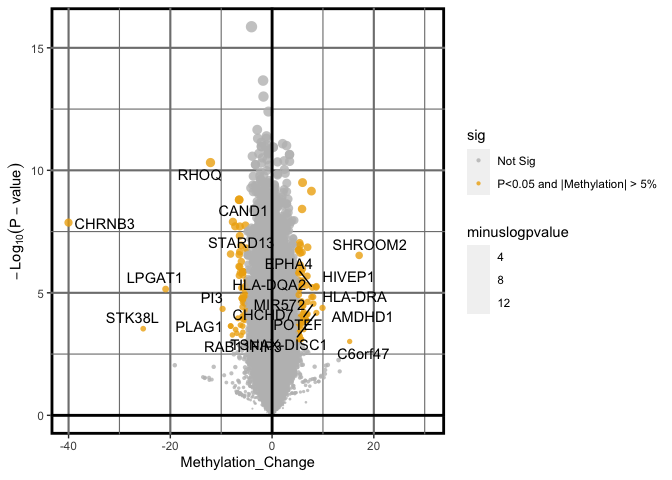
\includegraphics{README_files/figure-latex/Volcano-1.pdf}

\hypertarget{combined-analysis---biopsy-and-ipsc}{%
\section{Combined Analysis - Biopsy and
iPSC}\label{combined-analysis---biopsy-and-ipsc}}

\begin{Shaded}
\begin{Highlighting}[]
\FunctionTok{library}\NormalTok{(openxlsx)}
\FunctionTok{library}\NormalTok{(dplyr)}
\FunctionTok{library}\NormalTok{(tidyr)}
\FunctionTok{library}\NormalTok{(ComplexHeatmap)}
\FunctionTok{library}\NormalTok{(minfi)}
\NormalTok{NUMBER }\OtherTok{=} \DecValTok{20}
\NormalTok{STAT }\OtherTok{=} \FloatTok{0.001}
\CommentTok{\#Index}
\NormalTok{AnnoTargets}\OtherTok{\textless{}{-}}\FunctionTok{read.metharray.sheet}\NormalTok{(}\AttributeTok{base=}\StringTok{"../1\_Input/IDAT"}\NormalTok{, }\AttributeTok{pattern=}\StringTok{".csv"}\NormalTok{)}
\end{Highlighting}
\end{Shaded}

\begin{verbatim}
## [1] "../1_Input/IDAT/SampleSheet.csv"
\end{verbatim}

\begin{Shaded}
\begin{Highlighting}[]
\FunctionTok{rownames}\NormalTok{(AnnoTargets)}\OtherTok{\textless{}{-}}\NormalTok{AnnoTargets}\SpecialCharTok{$}\NormalTok{Sample\_Name}
\NormalTok{Index\_combined}\OtherTok{\textless{}{-}}\NormalTok{AnnoTargets }\SpecialCharTok{\%\textgreater{}\%}\NormalTok{ dplyr}\SpecialCharTok{::}\FunctionTok{select}\NormalTok{(Sample\_Group, Tissue, Sample\_ID)}
\CommentTok{\#iPSC Data}
\NormalTok{DMPs\_iPSC}\OtherTok{\textless{}{-}}\FunctionTok{read.xlsx}\NormalTok{(}\StringTok{"../2\_Output/iPSC\_DCM\_vs\_CON/iPSC\_DCM\_vs\_CON\_DMPs.xlsx"}\NormalTok{, }\AttributeTok{sheet =} \StringTok{"P\_0.05"}\NormalTok{, }\AttributeTok{rowNames =}\NormalTok{ T)}
\NormalTok{iPSC\_stats}\OtherTok{\textless{}{-}}\NormalTok{DMPs\_iPSC }\SpecialCharTok{\%\textgreater{}\%}\NormalTok{ dplyr}\SpecialCharTok{::}\FunctionTok{select}\NormalTok{(}\AttributeTok{Methylation\_iPSC =}\NormalTok{ Methylation.Diff, }\AttributeTok{pval\_iPSC =}\NormalTok{ pval, }\AttributeTok{adj.P.Val\_iPSC =}\NormalTok{ qval, Name}\SpecialCharTok{:}\NormalTok{Regulatory\_Feature\_Group)}


\CommentTok{\#biopsies}
\NormalTok{DMPs\_heart}\OtherTok{\textless{}{-}}\FunctionTok{read.xlsx}\NormalTok{(}\StringTok{"../2\_Output/heart\_DCM\_vs\_CON/heart\_DCM\_vs\_CON\_DMPs.xlsx"}\NormalTok{, }\AttributeTok{sheet =} \StringTok{"P\_0.05"}\NormalTok{, }\AttributeTok{rowNames =}\NormalTok{ T)}
\NormalTok{heart\_stats}\OtherTok{\textless{}{-}}\NormalTok{DMPs\_heart }\SpecialCharTok{\%\textgreater{}\%}\NormalTok{ dplyr}\SpecialCharTok{::}\FunctionTok{select}\NormalTok{(}\AttributeTok{Methylation\_heart =}\NormalTok{ Methylation.Diff, }\AttributeTok{pval\_heart =}\NormalTok{ pval, }\AttributeTok{adj.P.Val\_heart =}\NormalTok{ qval, Name}\SpecialCharTok{:}\NormalTok{Regulatory\_Feature\_Group)}
\NormalTok{heart\_index}\OtherTok{\textless{}{-}}\NormalTok{AnnoTargets }\SpecialCharTok{\%\textgreater{}\%}\NormalTok{ dplyr}\SpecialCharTok{::}\FunctionTok{filter}\NormalTok{(Tissue}\SpecialCharTok{==}\StringTok{"heart"}\NormalTok{) }\SpecialCharTok{\%\textgreater{}\%}\NormalTok{ dplyr}\SpecialCharTok{::}\FunctionTok{select}\NormalTok{(Tissue, Sample\_Group, Sample\_ID)}

\CommentTok{\#Beta}
\NormalTok{beta\_all}\OtherTok{\textless{}{-}}\FunctionTok{read.csv}\NormalTok{(}\StringTok{"../1\_Input/beta\_all.csv"}\NormalTok{, }\AttributeTok{row.names =} \DecValTok{1}\NormalTok{)}

\CommentTok{\#combine data}
\NormalTok{Combined\_DMPs}\OtherTok{\textless{}{-}}\FunctionTok{inner\_join}\NormalTok{(iPSC\_stats, heart\_stats)}
\NormalTok{Combined\_DMPs\_Separated}\OtherTok{\textless{}{-}}\NormalTok{Combined\_DMPs }\SpecialCharTok{\%\textgreater{}\%} \FunctionTok{mutate}\NormalTok{(}\AttributeTok{UCSC\_RefGene\_Name =} \FunctionTok{strsplit}\NormalTok{(}\FunctionTok{as.character}\NormalTok{(UCSC\_RefGene\_Name), }\StringTok{";"}\NormalTok{)) }\SpecialCharTok{\%\textgreater{}\%} \FunctionTok{unnest}\NormalTok{(UCSC\_RefGene\_Name) }\SpecialCharTok{\%\textgreater{}\%} \FunctionTok{distinct}\NormalTok{() }\SpecialCharTok{\%\textgreater{}\%} \FunctionTok{merge}\NormalTok{(., beta\_all, }\AttributeTok{by.x =} \StringTok{"Name"}\NormalTok{, }\AttributeTok{by.y =} \DecValTok{0}\NormalTok{)}

\CommentTok{\# Select only co{-}methylated positions (iPSC and heart)}
\NormalTok{Combined\_together}\OtherTok{\textless{}{-}}\NormalTok{Combined\_DMPs\_Separated }\SpecialCharTok{\%\textgreater{}\%} \FunctionTok{filter}\NormalTok{(Methylation\_iPSC}\SpecialCharTok{\textgreater{}}\DecValTok{0} \SpecialCharTok{\&}\NormalTok{ Methylation\_heart}\SpecialCharTok{\textgreater{}}\DecValTok{0} \SpecialCharTok{|}\NormalTok{ Methylation\_iPSC}\SpecialCharTok{\textless{}}\DecValTok{0} \SpecialCharTok{\&}\NormalTok{ Methylation\_heart}\SpecialCharTok{\textless{}}\DecValTok{0}\NormalTok{) }\SpecialCharTok{\%\textgreater{}\%} \FunctionTok{arrange}\NormalTok{(}\FunctionTok{desc}\NormalTok{(Methylation\_iPSC)) }\SpecialCharTok{\%\textgreater{}\%} \FunctionTok{filter}\NormalTok{(pval\_iPSC }\SpecialCharTok{\textless{}}\NormalTok{ STAT) }\SpecialCharTok{\%\textgreater{}\%} \FunctionTok{arrange}\NormalTok{(pval\_iPSC)}
\CommentTok{\#Find row number for top candidates}
\NormalTok{Candidates}\OtherTok{\textless{}{-}}\FunctionTok{which}\NormalTok{(Combined\_together}\SpecialCharTok{$}\NormalTok{UCSC\_RefGene\_Name }\SpecialCharTok{==} \StringTok{"ATG7"}\NormalTok{)}
\CommentTok{\# Combined\_together\textless{}{-}merge(Combined\_together, beta\_all, by.x = "Name", by.y = 0)}
\FunctionTok{rownames}\NormalTok{(Combined\_together)}\OtherTok{\textless{}{-}}\FunctionTok{make.unique}\NormalTok{(Combined\_together}\SpecialCharTok{$}\NormalTok{UCSC\_RefGene\_Name, }\AttributeTok{sep =} \StringTok{"."}\NormalTok{)}
\CommentTok{\#Create heatmap matrices and annotation}
\NormalTok{heart\_hm}\OtherTok{\textless{}{-}}\NormalTok{Combined\_together }\SpecialCharTok{\%\textgreater{}\%}\NormalTok{ dplyr}\SpecialCharTok{::}\FunctionTok{select}\NormalTok{(}\FunctionTok{contains}\NormalTok{(}\StringTok{"NF"}\NormalTok{) }\SpecialCharTok{|} \FunctionTok{contains}\NormalTok{(}\StringTok{"biopsy"}\NormalTok{)) }\SpecialCharTok{\%\textgreater{}\%} \FunctionTok{data.matrix}\NormalTok{()}
\NormalTok{heart\_index}\OtherTok{\textless{}{-}}\NormalTok{AnnoTargets }\SpecialCharTok{\%\textgreater{}\%}\NormalTok{ dplyr}\SpecialCharTok{::}\FunctionTok{filter}\NormalTok{(Tissue}\SpecialCharTok{==}\StringTok{"heart"}\NormalTok{) }\SpecialCharTok{\%\textgreater{}\%}\NormalTok{ dplyr}\SpecialCharTok{::}\FunctionTok{select}\NormalTok{(Tissue, Sample\_Group, Sample\_ID)}
\NormalTok{iPSC\_hm}\OtherTok{\textless{}{-}}\NormalTok{Combined\_together }\SpecialCharTok{\%\textgreater{}\%}\NormalTok{ dplyr}\SpecialCharTok{::}\FunctionTok{select}\NormalTok{(}\FunctionTok{contains}\NormalTok{(}\StringTok{"cells"}\NormalTok{) }\SpecialCharTok{\&} \FunctionTok{contains}\NormalTok{(}\StringTok{"co"}\NormalTok{),}\FunctionTok{contains}\NormalTok{(}\StringTok{"cells"}\NormalTok{) }\SpecialCharTok{\&} \FunctionTok{contains}\NormalTok{(}\StringTok{"go"}\NormalTok{), }\FunctionTok{contains}\NormalTok{(}\StringTok{"cells"}\NormalTok{) }\SpecialCharTok{\&} \FunctionTok{contains}\NormalTok{(}\StringTok{"bo"}\NormalTok{)) }\SpecialCharTok{\%\textgreater{}\%} \FunctionTok{data.matrix}\NormalTok{()}
\NormalTok{iPSC\_index}\OtherTok{\textless{}{-}}\NormalTok{AnnoTargets }\SpecialCharTok{\%\textgreater{}\%}\NormalTok{ dplyr}\SpecialCharTok{::}\FunctionTok{filter}\NormalTok{(Tissue}\SpecialCharTok{==}\StringTok{"iPSC"}\NormalTok{) }\SpecialCharTok{\%\textgreater{}\%}\NormalTok{ dplyr}\SpecialCharTok{::}\FunctionTok{select}\NormalTok{(Tissue, Sample\_Group, Sample\_ID)}
\FunctionTok{write.xlsx}\NormalTok{(Combined\_together, }\StringTok{"../2\_Output/Overlapping.DMPs\_iPSC.Biopsy.xlsx"}\NormalTok{, }\AttributeTok{overwrite =}\NormalTok{ T)}

\CommentTok{\# Venn Diagram}
\FunctionTok{library}\NormalTok{(VennDiagram)}
\NormalTok{futile.logger}\SpecialCharTok{::}\FunctionTok{flog.threshold}\NormalTok{(futile.logger}\SpecialCharTok{::}\NormalTok{ERROR, }\AttributeTok{name =} \StringTok{"VennDiagramLogger"}\NormalTok{)}
\end{Highlighting}
\end{Shaded}

\begin{verbatim}
## NULL
\end{verbatim}

\begin{Shaded}
\begin{Highlighting}[]
\NormalTok{x}\OtherTok{\textless{}{-}}\FunctionTok{list}\NormalTok{(}\AttributeTok{iPSC =}\NormalTok{ DMPs\_iPSC}\SpecialCharTok{$}\NormalTok{Name, }\AttributeTok{heart =}\NormalTok{ DMPs\_heart}\SpecialCharTok{$}\NormalTok{Name)}
\FunctionTok{venn.diagram}\NormalTok{(x,}\AttributeTok{fill =} \FunctionTok{c}\NormalTok{(}\StringTok{"darkgray"}\NormalTok{, }\StringTok{"firebrick2"}\NormalTok{), }\AttributeTok{alpha =} \FunctionTok{c}\NormalTok{(}\FloatTok{0.75}\NormalTok{, }\FloatTok{0.75}\NormalTok{), }\AttributeTok{lty =} \StringTok{\textquotesingle{}blank\textquotesingle{}}\NormalTok{, }\AttributeTok{filename =} \StringTok{"../2\_Output/Overlapping\_DMPs\_iPSC.Biopsy.png"}\NormalTok{, }\AttributeTok{na =} \StringTok{"remove"}\NormalTok{)}
\end{Highlighting}
\end{Shaded}

\begin{verbatim}
## [1] 1
\end{verbatim}

\begin{Shaded}
\begin{Highlighting}[]
\CommentTok{\# Heatmap}

\NormalTok{ann\_colors }\OtherTok{=} \FunctionTok{list}\NormalTok{(}\AttributeTok{Sample\_Group =} \FunctionTok{c}\NormalTok{(}\AttributeTok{DCM=}\StringTok{"\#1b9e77"}\NormalTok{, }\AttributeTok{CON =} \StringTok{"goldenrod2"}\NormalTok{), }\AttributeTok{Tissue =} \FunctionTok{c}\NormalTok{(}\AttributeTok{heart =} \StringTok{"coral2"}\NormalTok{, }\AttributeTok{iPSC =} \StringTok{"darkgray"}\NormalTok{), }\AttributeTok{Sample\_ID =} \FunctionTok{c}\NormalTok{(}\AttributeTok{A =} \StringTok{"white"}\NormalTok{, }\AttributeTok{B =} \StringTok{"orange"}\NormalTok{, }\AttributeTok{C =} \StringTok{"black"}\NormalTok{, }\AttributeTok{F =} \StringTok{"red"}\NormalTok{, }\AttributeTok{G =} \StringTok{"green"}\NormalTok{, }\AttributeTok{T =} \StringTok{"blue"}\NormalTok{, }\AttributeTok{V =} \StringTok{"purple"}\NormalTok{))}
\NormalTok{paletteLength }\OtherTok{\textless{}{-}} \DecValTok{100}
\NormalTok{myColor }\OtherTok{\textless{}{-}} \FunctionTok{colorRampPalette}\NormalTok{(}\FunctionTok{c}\NormalTok{(}\StringTok{"dodgerblue4"}\NormalTok{, }\StringTok{"white"}\NormalTok{, }\StringTok{"gold2"}\NormalTok{))(paletteLength)}

\CommentTok{\#iPSC}
\NormalTok{heatmap\_iPSC}\OtherTok{\textless{}{-}}\NormalTok{ComplexHeatmap}\SpecialCharTok{::}\FunctionTok{pheatmap}\NormalTok{(iPSC\_hm, }\AttributeTok{scale=}\StringTok{"row"}\NormalTok{,}
                    \AttributeTok{cluster\_cols =}\NormalTok{ F,}
                    \AttributeTok{cluster\_rows =}\NormalTok{ T,}
                     \CommentTok{\# angle\_col = 45,}
                     \AttributeTok{fontsize\_col =} \DecValTok{8}\NormalTok{,}
                     \AttributeTok{color =}\NormalTok{ myColor,}
                    \AttributeTok{annotation\_names\_col =} \ConstantTok{FALSE}\NormalTok{,}
                     \AttributeTok{show\_rownames =}\NormalTok{ F,}
                     \AttributeTok{border\_color =} \ConstantTok{NA}\NormalTok{,}
                    \AttributeTok{annotation\_colors =}\NormalTok{ ann\_colors,}
                    \AttributeTok{annotation\_col =}\NormalTok{ iPSC\_index)}
\NormalTok{heatmap\_iPSC}


\NormalTok{ha }\OtherTok{=} \FunctionTok{rowAnnotation}\NormalTok{(}\AttributeTok{foo =} \FunctionTok{anno\_mark}\NormalTok{(}\AttributeTok{at =} \FunctionTok{c}\NormalTok{(}\DecValTok{1}\SpecialCharTok{:}\DecValTok{10}\NormalTok{), }\AttributeTok{labels =}\NormalTok{ Combined\_together}\SpecialCharTok{$}\NormalTok{UCSC\_RefGene\_Name[}\DecValTok{1}\SpecialCharTok{:}\DecValTok{10}\NormalTok{]))}

\CommentTok{\#heart}
\NormalTok{heatmap\_heart}\OtherTok{\textless{}{-}}\NormalTok{ComplexHeatmap}\SpecialCharTok{::}\FunctionTok{pheatmap}\NormalTok{(heart\_hm, }\AttributeTok{scale =} \StringTok{"row"}\NormalTok{,}
                    \AttributeTok{cluster\_cols =}\NormalTok{ F,}
                    \AttributeTok{cluster\_rows =}\NormalTok{ T,}
                     \CommentTok{\# angle\_col = 45,}
                     \AttributeTok{fontsize\_col =} \DecValTok{8}\NormalTok{,}
                     \AttributeTok{color =}\NormalTok{ myColor,}
                     \AttributeTok{show\_rownames =}\NormalTok{ F,}
                     \AttributeTok{border\_color =} \ConstantTok{NA}\NormalTok{,}
                    \AttributeTok{annotation\_names\_col =} \ConstantTok{FALSE}\NormalTok{,}
                    \AttributeTok{right\_annotation =}\NormalTok{ ha,}
                    \AttributeTok{annotation\_colors =}\NormalTok{ ann\_colors,}
                    \AttributeTok{annotation\_col =}\NormalTok{ heart\_index)}

\NormalTok{heatmap\_heart}
\NormalTok{heatmap\_iPSC }\SpecialCharTok{+}\NormalTok{ heatmap\_heart}

\FunctionTok{pdf}\NormalTok{(}\AttributeTok{file=}\StringTok{"../2\_Output/complexheatmap\_combined.pdf"}\NormalTok{, }\AttributeTok{height =} \DecValTok{5}\NormalTok{, }\AttributeTok{width =} \DecValTok{7}\NormalTok{, }\AttributeTok{onefile =}\NormalTok{ F)}
\NormalTok{heatmap\_iPSC }\SpecialCharTok{+}\NormalTok{ heatmap\_heart}
\FunctionTok{dev.off}\NormalTok{()}
\end{Highlighting}
\end{Shaded}

\begin{verbatim}
## pdf 
##   2
\end{verbatim}

\hypertarget{validation}{%
\section{Validation}\label{validation}}

\begin{Shaded}
\begin{Highlighting}[]
\CommentTok{\#Import Pepin et al. 2019 Combined methylation{-}RNA{-}sequencing dataset}
\NormalTok{Pepin\_DMPs}\OtherTok{\textless{}{-}}\FunctionTok{read.xlsx}\NormalTok{(}\StringTok{"../1\_Input/Validation/HF.Effect\_NR\_Pre.v.CON\_Annotated\_DiffMeth.xlsx"}\NormalTok{)}
\end{Highlighting}
\end{Shaded}

\hypertarget{motif-enrichment}{%
\section{Motif Enrichment}\label{motif-enrichment}}

\begin{Shaded}
\begin{Highlighting}[]
\DocumentationTok{\#\#\#\#\#\# Working example (from BED file)}
\FunctionTok{library}\NormalTok{(monaLisa)}
\FunctionTok{library}\NormalTok{(GenomicRanges)}
\FunctionTok{library}\NormalTok{(SummarizedExperiment)}
\FunctionTok{library}\NormalTok{(openxlsx)}
\FunctionTok{library}\NormalTok{(dplyr)}
\FunctionTok{library}\NormalTok{(TFBSTools)}
\FunctionTok{library}\NormalTok{(JASPAR2020)}
\FunctionTok{library}\NormalTok{(BSgenome.Hsapiens.UCSC.hg19)}
\NormalTok{mcparams }\OtherTok{\textless{}{-}}\NormalTok{ BiocParallel}\SpecialCharTok{::}\FunctionTok{MulticoreParam}\NormalTok{(10L) }\CommentTok{\#parallelization (10{-}core)}
\NormalTok{DMPs\_iPSC}\OtherTok{\textless{}{-}}\FunctionTok{read.xlsx}\NormalTok{(}\StringTok{"../3\_Results/Overlapping.DMPs\_iPSC.Biopsy.xlsx"}\NormalTok{, }\AttributeTok{startRow =} \DecValTok{2}\NormalTok{)}
\NormalTok{bed}\OtherTok{\textless{}{-}}\NormalTok{DMPs\_iPSC }\SpecialCharTok{\%\textgreater{}\%}\NormalTok{ dplyr}\SpecialCharTok{::}\FunctionTok{select}\NormalTok{(chr, pos, Methylation\_iPSC) }\SpecialCharTok{\%\textgreater{}\%} \FunctionTok{transmute}\NormalTok{(}\AttributeTok{seqnames=}\NormalTok{chr, }\AttributeTok{start=}\NormalTok{pos}\DecValTok{{-}20}\NormalTok{, }\AttributeTok{end=}\NormalTok{pos}\SpecialCharTok{+}\DecValTok{20}\NormalTok{, }\AttributeTok{width =} \DecValTok{41}\NormalTok{, }\AttributeTok{strand =} \StringTok{"*"}\NormalTok{, }\AttributeTok{deltaMeth=}\NormalTok{Methylation\_iPSC)}
\NormalTok{bed\_mr}\OtherTok{\textless{}{-}}\FunctionTok{as}\NormalTok{(bed, }\StringTok{"GRanges"}\NormalTok{)}
\CommentTok{\# define bins by differential methylation}
\NormalTok{bins }\OtherTok{\textless{}{-}} \FunctionTok{bin}\NormalTok{(}\AttributeTok{x =}\NormalTok{ bed\_mr}\SpecialCharTok{$}\NormalTok{deltaMeth, }\AttributeTok{binmode =} \StringTok{"equalN"}\NormalTok{, }\AttributeTok{nElement =} \DecValTok{100}\NormalTok{, }\AttributeTok{minAbsX =} \DecValTok{1}\NormalTok{)}
\FunctionTok{table}\NormalTok{(bins)}
\end{Highlighting}
\end{Shaded}

\begin{verbatim}
## bins
## [-6.06,-1.5]  (-1.5,1.02]  (1.02,7.75] 
##          100          226          100
\end{verbatim}

\begin{Shaded}
\begin{Highlighting}[]
\FunctionTok{pdf}\NormalTok{(}\FunctionTok{paste0}\NormalTok{(}\StringTok{"../2\_Output/\_bins.pdf"}\NormalTok{), }\AttributeTok{width =} \FloatTok{7.5}\NormalTok{, }\AttributeTok{height =} \DecValTok{5}\NormalTok{)}
\FunctionTok{plotBinDensity}\NormalTok{(bed\_mr}\SpecialCharTok{$}\NormalTok{deltaMeth, bins, }\AttributeTok{legend =} \StringTok{"topright"}\NormalTok{)}
\FunctionTok{dev.off}\NormalTok{()}
\end{Highlighting}
\end{Shaded}

\begin{verbatim}
## pdf 
##   2
\end{verbatim}

\begin{Shaded}
\begin{Highlighting}[]
\CommentTok{\# get PWMs from JASPAR}
\NormalTok{pwms }\OtherTok{\textless{}{-}} \FunctionTok{getMatrixSet}\NormalTok{(JASPAR2020,}
                     \AttributeTok{opts =} \FunctionTok{list}\NormalTok{(}\AttributeTok{matrixtype =} \StringTok{"PWM"}\NormalTok{,}
                                 \AttributeTok{tax\_group =} \StringTok{"vertebrates"}\NormalTok{))}
\CommentTok{\# trim bed file for sequenes that are consistent}
\NormalTok{lmrsel }\OtherTok{\textless{}{-}} \FunctionTok{trim}\NormalTok{(}\FunctionTok{resize}\NormalTok{(bed\_mr, }\AttributeTok{width =} \FunctionTok{median}\NormalTok{(}\FunctionTok{width}\NormalTok{(bed\_mr)), }\AttributeTok{fix =} \StringTok{"center"}\NormalTok{))}
\CommentTok{\# get sequences from mouse genome}
\NormalTok{lmrseqs }\OtherTok{\textless{}{-}} \FunctionTok{getSeq}\NormalTok{(BSgenome.Hsapiens.UCSC.hg19, bed\_mr)}
\CommentTok{\# GC proportion (bias)}
\FunctionTok{plotBinDiagnostics}\NormalTok{(}\AttributeTok{seqs =}\NormalTok{ lmrseqs, }\AttributeTok{bins =}\NormalTok{ bins, }\AttributeTok{aspect =} \StringTok{"GCfrac"}\NormalTok{)}
\end{Highlighting}
\end{Shaded}

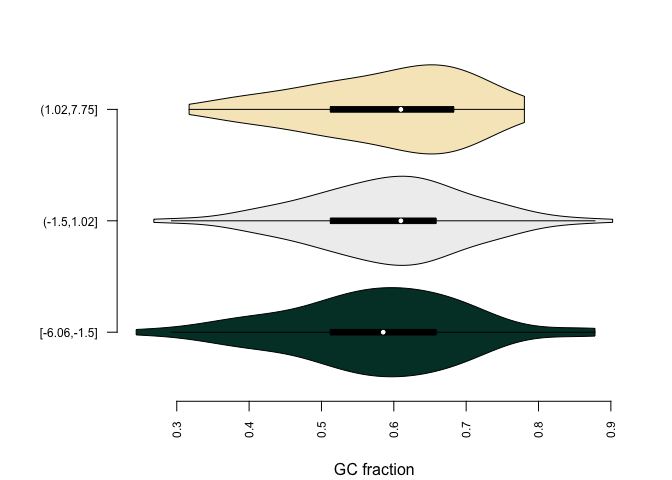
\includegraphics{README_files/figure-latex/motif-1.pdf}

\begin{Shaded}
\begin{Highlighting}[]
\FunctionTok{plotBinDiagnostics}\NormalTok{(}\AttributeTok{seqs =}\NormalTok{ lmrseqs, }\AttributeTok{bins =}\NormalTok{ bins, }\AttributeTok{aspect =} \StringTok{"dinucfreq"}\NormalTok{)}
\CommentTok{\# run motif enrichment}
\NormalTok{se }\OtherTok{\textless{}{-}} \FunctionTok{calcBinnedMotifEnrR}\NormalTok{(}\AttributeTok{seqs =}\NormalTok{ lmrseqs, }\AttributeTok{bins =}\NormalTok{ bins, }\AttributeTok{pwmL =}\NormalTok{ pwms, }\AttributeTok{BPPARAM =}\NormalTok{ BiocParallel}\SpecialCharTok{::}\FunctionTok{MulticoreParam}\NormalTok{(}\DecValTok{8}\NormalTok{))}
\CommentTok{\# Filter results}
\NormalTok{Test}\OtherTok{\textless{}{-}}\FunctionTok{as.data.frame}\NormalTok{(}\FunctionTok{assays}\NormalTok{(se))}
\NormalTok{sel }\OtherTok{\textless{}{-}} \FunctionTok{apply}\NormalTok{(}\FunctionTok{assay}\NormalTok{(se, }\StringTok{"negLog10P"}\NormalTok{), }\DecValTok{1}\NormalTok{, }
             \ControlFlowTok{function}\NormalTok{(x) }\FunctionTok{max}\NormalTok{(}\FunctionTok{abs}\NormalTok{(x), }\DecValTok{0}\NormalTok{, }\AttributeTok{na.rm =} \ConstantTok{TRUE}\NormalTok{)) }\SpecialCharTok{\textgreater{}} \FloatTok{1.0}
\FunctionTok{sum}\NormalTok{(sel)}
\end{Highlighting}
\end{Shaded}

\begin{verbatim}
## [1] 65
\end{verbatim}

\begin{Shaded}
\begin{Highlighting}[]
\CommentTok{\#\textgreater{} [1] 59}
\NormalTok{seSel }\OtherTok{\textless{}{-}}\NormalTok{ se[sel, ]}

\CommentTok{\# plot}
\FunctionTok{pdf}\NormalTok{(}\StringTok{"../2\_Output/Motifs.pdf"}\NormalTok{, }\AttributeTok{width =} \DecValTok{11}\NormalTok{, }\AttributeTok{height =} \DecValTok{10}\NormalTok{)}
\FunctionTok{plotMotifHeatmaps}\NormalTok{(}\AttributeTok{x =}\NormalTok{ seSel, }\AttributeTok{which.plots =} \FunctionTok{c}\NormalTok{(}\StringTok{"log2enr"}\NormalTok{, }\StringTok{"negLog10P"}\NormalTok{), }
                  \AttributeTok{width =} \FloatTok{2.0}\NormalTok{, }\AttributeTok{cluster =} \ConstantTok{TRUE}\NormalTok{, }\AttributeTok{maxEnr =} \DecValTok{2}\NormalTok{, }\AttributeTok{maxSig =} \DecValTok{10}\NormalTok{, }
                  \AttributeTok{show\_motif\_GC =} \ConstantTok{TRUE}\NormalTok{, }\AttributeTok{show\_dendrogram =}\NormalTok{ T,}\AttributeTok{show\_seqlogo =} \ConstantTok{TRUE}\NormalTok{)}
\FunctionTok{dev.off}\NormalTok{()}
\end{Highlighting}
\end{Shaded}

\begin{verbatim}
## pdf 
##   2
\end{verbatim}

\begin{Shaded}
\begin{Highlighting}[]
\FunctionTok{plotMotifHeatmaps}\NormalTok{(}\AttributeTok{x =}\NormalTok{ seSel, }\AttributeTok{which.plots =} \FunctionTok{c}\NormalTok{(}\StringTok{"log2enr"}\NormalTok{, }\StringTok{"negLog10P"}\NormalTok{), }
                  \AttributeTok{width =} \FloatTok{2.0}\NormalTok{, }\AttributeTok{cluster =} \ConstantTok{TRUE}\NormalTok{, }\AttributeTok{maxEnr =} \DecValTok{2}\NormalTok{, }\AttributeTok{maxSig =} \DecValTok{10}\NormalTok{, }
                  \AttributeTok{show\_motif\_GC =} \ConstantTok{TRUE}\NormalTok{, }\AttributeTok{show\_dendrogram =}\NormalTok{ T,}\AttributeTok{show\_seqlogo =} \ConstantTok{TRUE}\NormalTok{)}
\end{Highlighting}
\end{Shaded}

\hypertarget{supplemental-table-r-session-information}{%
\section{Supplemental Table: R Session
Information}\label{supplemental-table-r-session-information}}

All packages and setting are acquired using the following command:

\begin{Shaded}
\begin{Highlighting}[]
\FunctionTok{options}\NormalTok{(}\AttributeTok{kableExtra.latex.load\_packages =} \ConstantTok{FALSE}\NormalTok{)}
\NormalTok{Run\_tE}\OtherTok{\textless{}{-}}\FunctionTok{Sys.time}\NormalTok{()}
\NormalTok{Run\_time}\OtherTok{\textless{}{-}}\NormalTok{Run\_tE }\SpecialCharTok{{-}}\NormalTok{ Run\_tS}
\NormalTok{Run\_time}
\end{Highlighting}
\end{Shaded}

\begin{verbatim}
## Time difference of 23.60373 mins
\end{verbatim}

\begin{Shaded}
\begin{Highlighting}[]
\FunctionTok{library}\NormalTok{(kableExtra)}
\NormalTok{sinfo}\OtherTok{\textless{}{-}}\NormalTok{devtools}\SpecialCharTok{::}\FunctionTok{session\_info}\NormalTok{()}
\NormalTok{sinfo}\SpecialCharTok{$}\NormalTok{platform}
\end{Highlighting}
\end{Shaded}

\begin{verbatim}
##  setting  value
##  version  R version 4.1.2 (2021-11-01)
##  os       macOS Big Sur 10.16
##  system   x86_64, darwin17.0
##  ui       X11
##  language (EN)
##  collate  en_US.UTF-8
##  ctype    en_US.UTF-8
##  tz       Europe/Berlin
##  date     2022-01-03
##  pandoc   2.14.0.3 @ /Applications/RStudio.app/Contents/MacOS/pandoc/ (via rmarkdown)
\end{verbatim}

\begin{Shaded}
\begin{Highlighting}[]
\NormalTok{sinfo}\SpecialCharTok{$}\NormalTok{packages }\SpecialCharTok{\%\textgreater{}\%} \FunctionTok{kable}\NormalTok{( }
                         \AttributeTok{align=}\StringTok{"c"}\NormalTok{, }
                         \AttributeTok{caption=}\StringTok{"Packages and Required Dependencies"}\NormalTok{) }\SpecialCharTok{\%\textgreater{}\%} 
    \FunctionTok{kable\_styling}\NormalTok{(}\AttributeTok{latex\_options=}\FunctionTok{c}\NormalTok{(}\StringTok{"repeat\_header"}\NormalTok{, }\StringTok{"condensed"}\NormalTok{))}
\end{Highlighting}
\end{Shaded}

\begin{table}

\caption{\label{tab:settings}Packages and Required Dependencies}
\centering
\begin{tabular}[t]{l|c|c|c|c|c|c|c|c|c|c|c}
\hline
  & package & ondiskversion & loadedversion & path & loadedpath & attached & is\_base & date & source & md5ok & library\\
\hline
abind & abind & 1.4.5 & 1.4-5 & /Library/Frameworks/R.framework/Versions/4.1/Resources/library/abind & /Library/Frameworks/R.framework/Versions/4.1/Resources/library/abind & FALSE & FALSE & 2016-07-21 & CRAN (R 4.1.0) &  & /Library/Frameworks/R.framework/Versions/4.1/Resources/library\\
\hline
annotate & annotate & 1.72.0 & 1.72.0 & /Library/Frameworks/R.framework/Versions/4.1/Resources/library/annotate & /Library/Frameworks/R.framework/Versions/4.1/Resources/library/annotate & FALSE & FALSE & 2021-10-26 & Bioconductor &  & /Library/Frameworks/R.framework/Versions/4.1/Resources/library\\
\hline
AnnotationDbi & AnnotationDbi & 1.56.2 & 1.56.2 & /Library/Frameworks/R.framework/Versions/4.1/Resources/library/AnnotationDbi & /Library/Frameworks/R.framework/Versions/4.1/Resources/library/AnnotationDbi & TRUE & FALSE & 2021-11-09 & Bioconductor &  & /Library/Frameworks/R.framework/Versions/4.1/Resources/library\\
\hline
askpass & askpass & 1.1 & 1.1 & /Library/Frameworks/R.framework/Versions/4.1/Resources/library/askpass & /Library/Frameworks/R.framework/Versions/4.1/Resources/library/askpass & FALSE & FALSE & 2019-01-13 & CRAN (R 4.1.0) &  & /Library/Frameworks/R.framework/Versions/4.1/Resources/library\\
\hline
assertthat & assertthat & 0.2.1 & 0.2.1 & /Library/Frameworks/R.framework/Versions/4.1/Resources/library/assertthat & /Library/Frameworks/R.framework/Versions/4.1/Resources/library/assertthat & FALSE & FALSE & 2019-03-21 & CRAN (R 4.1.0) &  & /Library/Frameworks/R.framework/Versions/4.1/Resources/library\\
\hline
backports & backports & 1.4.0 & 1.4.0 & /Library/Frameworks/R.framework/Versions/4.1/Resources/library/backports & /Library/Frameworks/R.framework/Versions/4.1/Resources/library/backports & FALSE & FALSE & 2021-11-23 & CRAN (R 4.1.0) &  & /Library/Frameworks/R.framework/Versions/4.1/Resources/library\\
\hline
base64 & base64 & 2.0 & 2.0 & /Library/Frameworks/R.framework/Versions/4.1/Resources/library/base64 & /Library/Frameworks/R.framework/Versions/4.1/Resources/library/base64 & FALSE & FALSE & 2016-05-10 & CRAN (R 4.1.0) &  & /Library/Frameworks/R.framework/Versions/4.1/Resources/library\\
\hline
base64enc & base64enc & 0.1.3 & 0.1-3 & /Library/Frameworks/R.framework/Versions/4.1/Resources/library/base64enc & /Library/Frameworks/R.framework/Versions/4.1/Resources/library/base64enc & FALSE & FALSE & 2015-07-28 & CRAN (R 4.1.0) &  & /Library/Frameworks/R.framework/Versions/4.1/Resources/library\\
\hline
beanplot & beanplot & 1.2 & 1.2 & /Library/Frameworks/R.framework/Versions/4.1/Resources/library/beanplot & /Library/Frameworks/R.framework/Versions/4.1/Resources/library/beanplot & FALSE & FALSE & 2014-09-19 & CRAN (R 4.1.0) &  & /Library/Frameworks/R.framework/Versions/4.1/Resources/library\\
\hline
Biobase & Biobase & 2.54.0 & 2.54.0 & /Library/Frameworks/R.framework/Versions/4.1/Resources/library/Biobase & /Library/Frameworks/R.framework/Versions/4.1/Resources/library/Biobase & TRUE & FALSE & 2021-10-26 & Bioconductor &  & /Library/Frameworks/R.framework/Versions/4.1/Resources/library\\
\hline
BiocFileCache & BiocFileCache & 2.2.0 & 2.2.0 & /Library/Frameworks/R.framework/Versions/4.1/Resources/library/BiocFileCache & /Library/Frameworks/R.framework/Versions/4.1/Resources/library/BiocFileCache & FALSE & FALSE & 2021-10-26 & Bioconductor &  & /Library/Frameworks/R.framework/Versions/4.1/Resources/library\\
\hline
BiocGenerics & BiocGenerics & 0.40.0 & 0.40.0 & /Library/Frameworks/R.framework/Versions/4.1/Resources/library/BiocGenerics & /Library/Frameworks/R.framework/Versions/4.1/Resources/library/BiocGenerics & TRUE & FALSE & 2021-10-26 & Bioconductor &  & /Library/Frameworks/R.framework/Versions/4.1/Resources/library\\
\hline
BiocIO & BiocIO & 1.4.0 & 1.4.0 & /Library/Frameworks/R.framework/Versions/4.1/Resources/library/BiocIO & /Library/Frameworks/R.framework/Versions/4.1/Resources/library/BiocIO & FALSE & FALSE & 2021-10-26 & Bioconductor &  & /Library/Frameworks/R.framework/Versions/4.1/Resources/library\\
\hline
BiocParallel & BiocParallel & 1.28.2 & 1.28.2 & /Library/Frameworks/R.framework/Versions/4.1/Resources/library/BiocParallel & /Library/Frameworks/R.framework/Versions/4.1/Resources/library/BiocParallel & FALSE & FALSE & 2021-11-25 & Bioconductor &  & /Library/Frameworks/R.framework/Versions/4.1/Resources/library\\
\hline
biomaRt & biomaRt & 2.50.1 & 2.50.1 & /Library/Frameworks/R.framework/Versions/4.1/Resources/library/biomaRt & /Library/Frameworks/R.framework/Versions/4.1/Resources/library/biomaRt & TRUE & FALSE & 2021-11-21 & Bioconductor &  & /Library/Frameworks/R.framework/Versions/4.1/Resources/library\\
\hline
Biostrings & Biostrings & 2.62.0 & 2.62.0 & /Library/Frameworks/R.framework/Versions/4.1/Resources/library/Biostrings & /Library/Frameworks/R.framework/Versions/4.1/Resources/library/Biostrings & TRUE & FALSE & 2021-10-26 & Bioconductor &  & /Library/Frameworks/R.framework/Versions/4.1/Resources/library\\
\hline
bit & bit & 4.0.4 & 4.0.4 & /Library/Frameworks/R.framework/Versions/4.1/Resources/library/bit & /Library/Frameworks/R.framework/Versions/4.1/Resources/library/bit & FALSE & FALSE & 2020-08-04 & CRAN (R 4.1.0) &  & /Library/Frameworks/R.framework/Versions/4.1/Resources/library\\
\hline
bit64 & bit64 & 4.0.5 & 4.0.5 & /Library/Frameworks/R.framework/Versions/4.1/Resources/library/bit64 & /Library/Frameworks/R.framework/Versions/4.1/Resources/library/bit64 & FALSE & FALSE & 2020-08-30 & CRAN (R 4.1.0) &  & /Library/Frameworks/R.framework/Versions/4.1/Resources/library\\
\hline
bitops & bitops & 1.0.7 & 1.0-7 & /Library/Frameworks/R.framework/Versions/4.1/Resources/library/bitops & /Library/Frameworks/R.framework/Versions/4.1/Resources/library/bitops & FALSE & FALSE & 2021-04-24 & CRAN (R 4.1.0) &  & /Library/Frameworks/R.framework/Versions/4.1/Resources/library\\
\hline
blob & blob & 1.2.2 & 1.2.2 & /Library/Frameworks/R.framework/Versions/4.1/Resources/library/blob & /Library/Frameworks/R.framework/Versions/4.1/Resources/library/blob & FALSE & FALSE & 2021-07-23 & CRAN (R 4.1.0) &  & /Library/Frameworks/R.framework/Versions/4.1/Resources/library\\
\hline
broom & broom & 0.7.10 & 0.7.10 & /Library/Frameworks/R.framework/Versions/4.1/Resources/library/broom & /Library/Frameworks/R.framework/Versions/4.1/Resources/library/broom & FALSE & FALSE & 2021-10-31 & CRAN (R 4.1.0) &  & /Library/Frameworks/R.framework/Versions/4.1/Resources/library\\
\hline
BSgenome & BSgenome & 1.62.0 & 1.62.0 & /Library/Frameworks/R.framework/Versions/4.1/Resources/library/BSgenome & /Library/Frameworks/R.framework/Versions/4.1/Resources/library/BSgenome & TRUE & FALSE & 2021-10-26 & Bioconductor &  & /Library/Frameworks/R.framework/Versions/4.1/Resources/library\\
\hline
BSgenome.Hsapiens.UCSC.hg19 & BSgenome.Hsapiens.UCSC.hg19 & 1.4.3 & 1.4.3 & /Library/Frameworks/R.framework/Versions/4.1/Resources/library/BSgenome.Hsapiens.UCSC.hg19 & /Library/Frameworks/R.framework/Versions/4.1/Resources/library/BSgenome.Hsapiens.UCSC.hg19 & TRUE & FALSE & 2021-12-02 & Bioconductor &  & /Library/Frameworks/R.framework/Versions/4.1/Resources/library\\
\hline
bumphunter & bumphunter & 1.36.0 & 1.36.0 & /Library/Frameworks/R.framework/Versions/4.1/Resources/library/bumphunter & /Library/Frameworks/R.framework/Versions/4.1/Resources/library/bumphunter & TRUE & FALSE & 2021-10-26 & Bioconductor &  & /Library/Frameworks/R.framework/Versions/4.1/Resources/library\\
\hline
cachem & cachem & 1.0.6 & 1.0.6 & /Library/Frameworks/R.framework/Versions/4.1/Resources/library/cachem & /Library/Frameworks/R.framework/Versions/4.1/Resources/library/cachem & FALSE & FALSE & 2021-08-19 & CRAN (R 4.1.0) &  & /Library/Frameworks/R.framework/Versions/4.1/Resources/library\\
\hline
calibrate & calibrate & 1.7.7 & 1.7.7 & /Library/Frameworks/R.framework/Versions/4.1/Resources/library/calibrate & /Library/Frameworks/R.framework/Versions/4.1/Resources/library/calibrate & TRUE & FALSE & 2020-06-19 & CRAN (R 4.1.0) &  & /Library/Frameworks/R.framework/Versions/4.1/Resources/library\\
\hline
callr & callr & 3.7.0 & 3.7.0 & /Library/Frameworks/R.framework/Versions/4.1/Resources/library/callr & /Library/Frameworks/R.framework/Versions/4.1/Resources/library/callr & FALSE & FALSE & 2021-04-20 & CRAN (R 4.1.0) &  & /Library/Frameworks/R.framework/Versions/4.1/Resources/library\\
\hline
car & car & 3.0.12 & 3.0-12 & /Library/Frameworks/R.framework/Versions/4.1/Resources/library/car & /Library/Frameworks/R.framework/Versions/4.1/Resources/library/car & FALSE & FALSE & 2021-11-06 & CRAN (R 4.1.0) &  & /Library/Frameworks/R.framework/Versions/4.1/Resources/library\\
\hline
carData & carData & 3.0.4 & 3.0-4 & /Library/Frameworks/R.framework/Versions/4.1/Resources/library/carData & /Library/Frameworks/R.framework/Versions/4.1/Resources/library/carData & FALSE & FALSE & 2020-05-22 & CRAN (R 4.1.0) &  & /Library/Frameworks/R.framework/Versions/4.1/Resources/library\\
\hline
caTools & caTools & 1.18.2 & 1.18.2 & /Library/Frameworks/R.framework/Versions/4.1/Resources/library/caTools & /Library/Frameworks/R.framework/Versions/4.1/Resources/library/caTools & FALSE & FALSE & 2021-03-28 & CRAN (R 4.1.0) &  & /Library/Frameworks/R.framework/Versions/4.1/Resources/library\\
\hline
cellranger & cellranger & 1.1.0 & 1.1.0 & /Library/Frameworks/R.framework/Versions/4.1/Resources/library/cellranger & /Library/Frameworks/R.framework/Versions/4.1/Resources/library/cellranger & FALSE & FALSE & 2016-07-27 & CRAN (R 4.1.0) &  & /Library/Frameworks/R.framework/Versions/4.1/Resources/library\\
\hline
checkmate & checkmate & 2.0.0 & 2.0.0 & /Library/Frameworks/R.framework/Versions/4.1/Resources/library/checkmate & /Library/Frameworks/R.framework/Versions/4.1/Resources/library/checkmate & FALSE & FALSE & 2020-02-06 & CRAN (R 4.1.0) &  & /Library/Frameworks/R.framework/Versions/4.1/Resources/library\\
\hline
circlize & circlize & 0.4.13 & 0.4.13 & /Library/Frameworks/R.framework/Versions/4.1/Resources/library/circlize & /Library/Frameworks/R.framework/Versions/4.1/Resources/library/circlize & FALSE & FALSE & 2021-06-09 & CRAN (R 4.1.0) &  & /Library/Frameworks/R.framework/Versions/4.1/Resources/library\\
\hline
cli & cli & 3.1.0 & 3.1.0 & /Library/Frameworks/R.framework/Versions/4.1/Resources/library/cli & /Library/Frameworks/R.framework/Versions/4.1/Resources/library/cli & FALSE & FALSE & 2021-10-27 & CRAN (R 4.1.0) &  & /Library/Frameworks/R.framework/Versions/4.1/Resources/library\\
\hline
clue & clue & 0.3.60 & 0.3-60 & /Library/Frameworks/R.framework/Versions/4.1/Resources/library/clue & /Library/Frameworks/R.framework/Versions/4.1/Resources/library/clue & FALSE & FALSE & 2021-10-11 & CRAN (R 4.1.0) &  & /Library/Frameworks/R.framework/Versions/4.1/Resources/library\\
\hline
cluster & cluster & 2.1.2 & 2.1.2 & /Library/Frameworks/R.framework/Versions/4.1/Resources/library/cluster & /Library/Frameworks/R.framework/Versions/4.1/Resources/library/cluster & FALSE & FALSE & 2021-04-17 & CRAN (R 4.1.2) &  & /Library/Frameworks/R.framework/Versions/4.1/Resources/library\\
\hline
CNEr & CNEr & 1.30.0 & 1.30.0 & /Library/Frameworks/R.framework/Versions/4.1/Resources/library/CNEr & /Library/Frameworks/R.framework/Versions/4.1/Resources/library/CNEr & FALSE & FALSE & 2021-10-26 & Bioconductor &  & /Library/Frameworks/R.framework/Versions/4.1/Resources/library\\
\hline
codetools & codetools & 0.2.18 & 0.2-18 & /Library/Frameworks/R.framework/Versions/4.1/Resources/library/codetools & /Library/Frameworks/R.framework/Versions/4.1/Resources/library/codetools & FALSE & FALSE & 2020-11-04 & CRAN (R 4.1.2) &  & /Library/Frameworks/R.framework/Versions/4.1/Resources/library\\
\hline
colorspace & colorspace & 2.0.2 & 2.0-2 & /Library/Frameworks/R.framework/Versions/4.1/Resources/library/colorspace & /Library/Frameworks/R.framework/Versions/4.1/Resources/library/colorspace & FALSE & FALSE & 2021-06-24 & CRAN (R 4.1.0) &  & /Library/Frameworks/R.framework/Versions/4.1/Resources/library\\
\hline
ComplexHeatmap & ComplexHeatmap & 2.11.1 & 2.11.1 & /Library/Frameworks/R.framework/Versions/4.1/Resources/library/ComplexHeatmap & /Library/Frameworks/R.framework/Versions/4.1/Resources/library/ComplexHeatmap & TRUE & FALSE & 2021-11-26 & Github (jokergoo/ComplexHeatmap@826b321) &  & /Library/Frameworks/R.framework/Versions/4.1/Resources/library\\
\hline
corrplot & corrplot & 0.92 & 0.92 & /Library/Frameworks/R.framework/Versions/4.1/Resources/library/corrplot & /Library/Frameworks/R.framework/Versions/4.1/Resources/library/corrplot & TRUE & FALSE & 2021-11-18 & CRAN (R 4.1.0) &  & /Library/Frameworks/R.framework/Versions/4.1/Resources/library\\
\hline
cowplot & cowplot & 1.1.1 & 1.1.1 & /Library/Frameworks/R.framework/Versions/4.1/Resources/library/cowplot & /Library/Frameworks/R.framework/Versions/4.1/Resources/library/cowplot & TRUE & FALSE & 2020-12-30 & CRAN (R 4.1.0) &  & /Library/Frameworks/R.framework/Versions/4.1/Resources/library\\
\hline
crayon & crayon & 1.4.2 & 1.4.2 & /Library/Frameworks/R.framework/Versions/4.1/Resources/library/crayon & /Library/Frameworks/R.framework/Versions/4.1/Resources/library/crayon & FALSE & FALSE & 2021-10-29 & CRAN (R 4.1.0) &  & /Library/Frameworks/R.framework/Versions/4.1/Resources/library\\
\hline
crosstalk & crosstalk & 1.2.0 & 1.2.0 & /Library/Frameworks/R.framework/Versions/4.1/Resources/library/crosstalk & /Library/Frameworks/R.framework/Versions/4.1/Resources/library/crosstalk & FALSE & FALSE & 2021-11-04 & CRAN (R 4.1.0) &  & /Library/Frameworks/R.framework/Versions/4.1/Resources/library\\
\hline
curl & curl & 4.3.2 & 4.3.2 & /Library/Frameworks/R.framework/Versions/4.1/Resources/library/curl & /Library/Frameworks/R.framework/Versions/4.1/Resources/library/curl & FALSE & FALSE & 2021-06-23 & CRAN (R 4.1.0) &  & /Library/Frameworks/R.framework/Versions/4.1/Resources/library\\
\hline
data.table & data.table & 1.14.2 & 1.14.2 & /Library/Frameworks/R.framework/Versions/4.1/Resources/library/data.table & /Library/Frameworks/R.framework/Versions/4.1/Resources/library/data.table & TRUE & FALSE & 2021-09-27 & CRAN (R 4.1.0) &  & /Library/Frameworks/R.framework/Versions/4.1/Resources/library\\
\hline
DBI & DBI & 1.1.1 & 1.1.1 & /Library/Frameworks/R.framework/Versions/4.1/Resources/library/DBI & /Library/Frameworks/R.framework/Versions/4.1/Resources/library/DBI & FALSE & FALSE & 2021-01-15 & CRAN (R 4.1.0) &  & /Library/Frameworks/R.framework/Versions/4.1/Resources/library\\
\hline
dbplyr & dbplyr & 2.1.1 & 2.1.1 & /Library/Frameworks/R.framework/Versions/4.1/Resources/library/dbplyr & /Library/Frameworks/R.framework/Versions/4.1/Resources/library/dbplyr & FALSE & FALSE & 2021-04-06 & CRAN (R 4.1.0) &  & /Library/Frameworks/R.framework/Versions/4.1/Resources/library\\
\hline
DelayedArray & DelayedArray & 0.20.0 & 0.20.0 & /Library/Frameworks/R.framework/Versions/4.1/Resources/library/DelayedArray & /Library/Frameworks/R.framework/Versions/4.1/Resources/library/DelayedArray & FALSE & FALSE & 2021-10-26 & Bioconductor &  & /Library/Frameworks/R.framework/Versions/4.1/Resources/library\\
\hline
DelayedMatrixStats & DelayedMatrixStats & 1.16.0 & 1.16.0 & /Library/Frameworks/R.framework/Versions/4.1/Resources/library/DelayedMatrixStats & /Library/Frameworks/R.framework/Versions/4.1/Resources/library/DelayedMatrixStats & FALSE & FALSE & 2021-10-26 & Bioconductor &  & /Library/Frameworks/R.framework/Versions/4.1/Resources/library\\
\hline
desc & desc & 1.4.0 & 1.4.0 & /Library/Frameworks/R.framework/Versions/4.1/Resources/library/desc & /Library/Frameworks/R.framework/Versions/4.1/Resources/library/desc & FALSE & FALSE & 2021-09-28 & CRAN (R 4.1.0) &  & /Library/Frameworks/R.framework/Versions/4.1/Resources/library\\
\hline
DESeq2 & DESeq2 & 1.34.0 & 1.34.0 & /Library/Frameworks/R.framework/Versions/4.1/Resources/library/DESeq2 & /Library/Frameworks/R.framework/Versions/4.1/Resources/library/DESeq2 & TRUE & FALSE & 2021-10-26 & Bioconductor &  & /Library/Frameworks/R.framework/Versions/4.1/Resources/library\\
\hline
devtools & devtools & 2.4.3 & 2.4.3 & /Library/Frameworks/R.framework/Versions/4.1/Resources/library/devtools & /Library/Frameworks/R.framework/Versions/4.1/Resources/library/devtools & FALSE & FALSE & 2021-11-30 & CRAN (R 4.1.0) &  & /Library/Frameworks/R.framework/Versions/4.1/Resources/library\\
\hline
digest & digest & 0.6.29 & 0.6.29 & /Library/Frameworks/R.framework/Versions/4.1/Resources/library/digest & /Library/Frameworks/R.framework/Versions/4.1/Resources/library/digest & FALSE & FALSE & 2021-12-01 & CRAN (R 4.1.0) &  & /Library/Frameworks/R.framework/Versions/4.1/Resources/library\\
\hline
DirichletMultinomial & DirichletMultinomial & 1.36.0 & 1.36.0 & /Library/Frameworks/R.framework/Versions/4.1/Resources/library/DirichletMultinomial & /Library/Frameworks/R.framework/Versions/4.1/Resources/library/DirichletMultinomial & FALSE & FALSE & 2021-10-26 & Bioconductor &  & /Library/Frameworks/R.framework/Versions/4.1/Resources/library\\
\hline
doParallel & doParallel & 1.0.16 & 1.0.16 & /Library/Frameworks/R.framework/Versions/4.1/Resources/library/doParallel & /Library/Frameworks/R.framework/Versions/4.1/Resources/library/doParallel & FALSE & FALSE & 2020-10-16 & CRAN (R 4.1.0) &  & /Library/Frameworks/R.framework/Versions/4.1/Resources/library\\
\hline
doRNG & doRNG & 1.8.2 & 1.8.2 & /Library/Frameworks/R.framework/Versions/4.1/Resources/library/doRNG & /Library/Frameworks/R.framework/Versions/4.1/Resources/library/doRNG & FALSE & FALSE & 2020-01-27 & CRAN (R 4.1.0) &  & /Library/Frameworks/R.framework/Versions/4.1/Resources/library\\
\hline
dplyr & dplyr & 1.0.7 & 1.0.7 & /Library/Frameworks/R.framework/Versions/4.1/Resources/library/dplyr & /Library/Frameworks/R.framework/Versions/4.1/Resources/library/dplyr & TRUE & FALSE & 2021-06-18 & CRAN (R 4.1.0) &  & /Library/Frameworks/R.framework/Versions/4.1/Resources/library\\
\hline
ellipsis & ellipsis & 0.3.2 & 0.3.2 & /Library/Frameworks/R.framework/Versions/4.1/Resources/library/ellipsis & /Library/Frameworks/R.framework/Versions/4.1/Resources/library/ellipsis & FALSE & FALSE & 2021-04-29 & CRAN (R 4.1.0) &  & /Library/Frameworks/R.framework/Versions/4.1/Resources/library\\
\hline
evaluate & evaluate & 0.14 & 0.14 & /Library/Frameworks/R.framework/Versions/4.1/Resources/library/evaluate & /Library/Frameworks/R.framework/Versions/4.1/Resources/library/evaluate & FALSE & FALSE & 2019-05-28 & CRAN (R 4.1.0) &  & /Library/Frameworks/R.framework/Versions/4.1/Resources/library\\
\hline
fansi & fansi & 0.5.0 & 0.5.0 & /Library/Frameworks/R.framework/Versions/4.1/Resources/library/fansi & /Library/Frameworks/R.framework/Versions/4.1/Resources/library/fansi & FALSE & FALSE & 2021-05-25 & CRAN (R 4.1.0) &  & /Library/Frameworks/R.framework/Versions/4.1/Resources/library\\
\hline
farver & farver & 2.1.0 & 2.1.0 & /Library/Frameworks/R.framework/Versions/4.1/Resources/library/farver & /Library/Frameworks/R.framework/Versions/4.1/Resources/library/farver & FALSE & FALSE & 2021-02-28 & CRAN (R 4.1.0) &  & /Library/Frameworks/R.framework/Versions/4.1/Resources/library\\
\hline
fastmap & fastmap & 1.1.0 & 1.1.0 & /Library/Frameworks/R.framework/Versions/4.1/Resources/library/fastmap & /Library/Frameworks/R.framework/Versions/4.1/Resources/library/fastmap & FALSE & FALSE & 2021-01-25 & CRAN (R 4.1.0) &  & /Library/Frameworks/R.framework/Versions/4.1/Resources/library\\
\hline
ff & ff & 4.0.5 & 4.0.5 & /Library/Frameworks/R.framework/Versions/4.1/Resources/library/ff & /Library/Frameworks/R.framework/Versions/4.1/Resources/library/ff & FALSE & FALSE & 2021-10-29 & CRAN (R 4.1.0) &  & /Library/Frameworks/R.framework/Versions/4.1/Resources/library\\
\hline
filelock & filelock & 1.0.2 & 1.0.2 & /Library/Frameworks/R.framework/Versions/4.1/Resources/library/filelock & /Library/Frameworks/R.framework/Versions/4.1/Resources/library/filelock & FALSE & FALSE & 2018-10-05 & CRAN (R 4.1.0) &  & /Library/Frameworks/R.framework/Versions/4.1/Resources/library\\
\hline
foreach & foreach & 1.5.1 & 1.5.1 & /Library/Frameworks/R.framework/Versions/4.1/Resources/library/foreach & /Library/Frameworks/R.framework/Versions/4.1/Resources/library/foreach & TRUE & FALSE & 2020-10-15 & CRAN (R 4.1.0) &  & /Library/Frameworks/R.framework/Versions/4.1/Resources/library\\
\hline
foreign & foreign & 0.8.81 & 0.8-81 & /Library/Frameworks/R.framework/Versions/4.1/Resources/library/foreign & /Library/Frameworks/R.framework/Versions/4.1/Resources/library/foreign & FALSE & FALSE & 2020-12-22 & CRAN (R 4.1.2) &  & /Library/Frameworks/R.framework/Versions/4.1/Resources/library\\
\hline
formatR & formatR & 1.11 & 1.11 & /Library/Frameworks/R.framework/Versions/4.1/Resources/library/formatR & /Library/Frameworks/R.framework/Versions/4.1/Resources/library/formatR & FALSE & FALSE & 2021-06-01 & CRAN (R 4.1.0) &  & /Library/Frameworks/R.framework/Versions/4.1/Resources/library\\
\hline
Formula & Formula & 1.2.4 & 1.2-4 & /Library/Frameworks/R.framework/Versions/4.1/Resources/library/Formula & /Library/Frameworks/R.framework/Versions/4.1/Resources/library/Formula & TRUE & FALSE & 2020-10-16 & CRAN (R 4.1.0) &  & /Library/Frameworks/R.framework/Versions/4.1/Resources/library\\
\hline
fs & fs & 1.5.1 & 1.5.1 & /Library/Frameworks/R.framework/Versions/4.1/Resources/library/fs & /Library/Frameworks/R.framework/Versions/4.1/Resources/library/fs & FALSE & FALSE & 2021-11-30 & CRAN (R 4.1.0) &  & /Library/Frameworks/R.framework/Versions/4.1/Resources/library\\
\hline
futile.logger & futile.logger & 1.4.3 & 1.4.3 & /Library/Frameworks/R.framework/Versions/4.1/Resources/library/futile.logger & /Library/Frameworks/R.framework/Versions/4.1/Resources/library/futile.logger & TRUE & FALSE & 2016-07-10 & CRAN (R 4.1.0) &  & /Library/Frameworks/R.framework/Versions/4.1/Resources/library\\
\hline
futile.options & futile.options & 1.0.1 & 1.0.1 & /Library/Frameworks/R.framework/Versions/4.1/Resources/library/futile.options & /Library/Frameworks/R.framework/Versions/4.1/Resources/library/futile.options & FALSE & FALSE & 2018-04-20 & CRAN (R 4.1.0) &  & /Library/Frameworks/R.framework/Versions/4.1/Resources/library\\
\hline
genefilter & genefilter & 1.76.0 & 1.76.0 & /Library/Frameworks/R.framework/Versions/4.1/Resources/library/genefilter & /Library/Frameworks/R.framework/Versions/4.1/Resources/library/genefilter & FALSE & FALSE & 2021-10-26 & Bioconductor &  & /Library/Frameworks/R.framework/Versions/4.1/Resources/library\\
\hline
geneplotter & geneplotter & 1.72.0 & 1.72.0 & /Library/Frameworks/R.framework/Versions/4.1/Resources/library/geneplotter & /Library/Frameworks/R.framework/Versions/4.1/Resources/library/geneplotter & FALSE & FALSE & 2021-10-26 & Bioconductor &  & /Library/Frameworks/R.framework/Versions/4.1/Resources/library\\
\hline
generics & generics & 0.1.1 & 0.1.1 & /Library/Frameworks/R.framework/Versions/4.1/Resources/library/generics & /Library/Frameworks/R.framework/Versions/4.1/Resources/library/generics & FALSE & FALSE & 2021-10-25 & CRAN (R 4.1.0) &  & /Library/Frameworks/R.framework/Versions/4.1/Resources/library\\
\hline
GenomeInfoDb & GenomeInfoDb & 1.30.0 & 1.30.0 & /Library/Frameworks/R.framework/Versions/4.1/Resources/library/GenomeInfoDb & /Library/Frameworks/R.framework/Versions/4.1/Resources/library/GenomeInfoDb & TRUE & FALSE & 2021-10-26 & Bioconductor &  & /Library/Frameworks/R.framework/Versions/4.1/Resources/library\\
\hline
GenomeInfoDbData & GenomeInfoDbData & 1.2.7 & 1.2.7 & /Library/Frameworks/R.framework/Versions/4.1/Resources/library/GenomeInfoDbData & /Library/Frameworks/R.framework/Versions/4.1/Resources/library/GenomeInfoDbData & FALSE & FALSE & 2021-11-17 & Bioconductor &  & /Library/Frameworks/R.framework/Versions/4.1/Resources/library\\
\hline
GenomicAlignments & GenomicAlignments & 1.30.0 & 1.30.0 & /Library/Frameworks/R.framework/Versions/4.1/Resources/library/GenomicAlignments & /Library/Frameworks/R.framework/Versions/4.1/Resources/library/GenomicAlignments & FALSE & FALSE & 2021-10-26 & Bioconductor &  & /Library/Frameworks/R.framework/Versions/4.1/Resources/library\\
\hline
GenomicFeatures & GenomicFeatures & 1.46.1 & 1.46.1 & /Library/Frameworks/R.framework/Versions/4.1/Resources/library/GenomicFeatures & /Library/Frameworks/R.framework/Versions/4.1/Resources/library/GenomicFeatures & TRUE & FALSE & 2021-10-27 & Bioconductor &  & /Library/Frameworks/R.framework/Versions/4.1/Resources/library\\
\hline
GenomicRanges & GenomicRanges & 1.46.1 & 1.46.1 & /Library/Frameworks/R.framework/Versions/4.1/Resources/library/GenomicRanges & /Library/Frameworks/R.framework/Versions/4.1/Resources/library/GenomicRanges & TRUE & FALSE & 2021-11-18 & Bioconductor &  & /Library/Frameworks/R.framework/Versions/4.1/Resources/library\\
\hline
GEOquery & GEOquery & 2.62.1 & 2.62.1 & /Library/Frameworks/R.framework/Versions/4.1/Resources/library/GEOquery & /Library/Frameworks/R.framework/Versions/4.1/Resources/library/GEOquery & FALSE & FALSE & 2021-11-16 & Bioconductor &  & /Library/Frameworks/R.framework/Versions/4.1/Resources/library\\
\hline
GetoptLong & GetoptLong & 1.0.5 & 1.0.5 & /Library/Frameworks/R.framework/Versions/4.1/Resources/library/GetoptLong & /Library/Frameworks/R.framework/Versions/4.1/Resources/library/GetoptLong & FALSE & FALSE & 2020-12-15 & CRAN (R 4.1.0) &  & /Library/Frameworks/R.framework/Versions/4.1/Resources/library\\
\hline
ggplot2 & ggplot2 & 3.3.5 & 3.3.5 & /Library/Frameworks/R.framework/Versions/4.1/Resources/library/ggplot2 & /Library/Frameworks/R.framework/Versions/4.1/Resources/library/ggplot2 & TRUE & FALSE & 2021-06-25 & CRAN (R 4.1.0) &  & /Library/Frameworks/R.framework/Versions/4.1/Resources/library\\
\hline
ggpubr & ggpubr & 0.4.0 & 0.4.0 & /Library/Frameworks/R.framework/Versions/4.1/Resources/library/ggpubr & /Library/Frameworks/R.framework/Versions/4.1/Resources/library/ggpubr & TRUE & FALSE & 2020-06-27 & CRAN (R 4.1.0) &  & /Library/Frameworks/R.framework/Versions/4.1/Resources/library\\
\hline
ggrepel & ggrepel & 0.9.1 & 0.9.1 & /Library/Frameworks/R.framework/Versions/4.1/Resources/library/ggrepel & /Library/Frameworks/R.framework/Versions/4.1/Resources/library/ggrepel & TRUE & FALSE & 2021-01-15 & CRAN (R 4.1.0) &  & /Library/Frameworks/R.framework/Versions/4.1/Resources/library\\
\hline
ggsignif & ggsignif & 0.6.3 & 0.6.3 & /Library/Frameworks/R.framework/Versions/4.1/Resources/library/ggsignif & /Library/Frameworks/R.framework/Versions/4.1/Resources/library/ggsignif & TRUE & FALSE & 2021-09-09 & CRAN (R 4.1.0) &  & /Library/Frameworks/R.framework/Versions/4.1/Resources/library\\
\hline
glmnet & glmnet & 4.1.3 & 4.1-3 & /Library/Frameworks/R.framework/Versions/4.1/Resources/library/glmnet & /Library/Frameworks/R.framework/Versions/4.1/Resources/library/glmnet & FALSE & FALSE & 2021-11-02 & CRAN (R 4.1.0) &  & /Library/Frameworks/R.framework/Versions/4.1/Resources/library\\
\hline
GlobalOptions & GlobalOptions & 0.1.2 & 0.1.2 & /Library/Frameworks/R.framework/Versions/4.1/Resources/library/GlobalOptions & /Library/Frameworks/R.framework/Versions/4.1/Resources/library/GlobalOptions & FALSE & FALSE & 2020-06-10 & CRAN (R 4.1.0) &  & /Library/Frameworks/R.framework/Versions/4.1/Resources/library\\
\hline
glue & glue & 1.5.1 & 1.5.1 & /Library/Frameworks/R.framework/Versions/4.1/Resources/library/glue & /Library/Frameworks/R.framework/Versions/4.1/Resources/library/glue & FALSE & FALSE & 2021-11-30 & CRAN (R 4.1.0) &  & /Library/Frameworks/R.framework/Versions/4.1/Resources/library\\
\hline
GO.db & GO.db & 3.14.0 & 3.14.0 & /Library/Frameworks/R.framework/Versions/4.1/Resources/library/GO.db & /Library/Frameworks/R.framework/Versions/4.1/Resources/library/GO.db & FALSE & FALSE & 2021-12-06 & Bioconductor &  & /Library/Frameworks/R.framework/Versions/4.1/Resources/library\\
\hline
gridExtra & gridExtra & 2.3 & 2.3 & /Library/Frameworks/R.framework/Versions/4.1/Resources/library/gridExtra & /Library/Frameworks/R.framework/Versions/4.1/Resources/library/gridExtra & TRUE & FALSE & 2017-09-09 & CRAN (R 4.1.0) &  & /Library/Frameworks/R.framework/Versions/4.1/Resources/library\\
\hline
gtable & gtable & 0.3.0 & 0.3.0 & /Library/Frameworks/R.framework/Versions/4.1/Resources/library/gtable & /Library/Frameworks/R.framework/Versions/4.1/Resources/library/gtable & FALSE & FALSE & 2019-03-25 & CRAN (R 4.1.0) &  & /Library/Frameworks/R.framework/Versions/4.1/Resources/library\\
\hline
gtools & gtools & 3.9.2 & 3.9.2 & /Library/Frameworks/R.framework/Versions/4.1/Resources/library/gtools & /Library/Frameworks/R.framework/Versions/4.1/Resources/library/gtools & TRUE & FALSE & 2021-06-06 & CRAN (R 4.1.0) &  & /Library/Frameworks/R.framework/Versions/4.1/Resources/library\\
\hline
Haplin & Haplin & 7.2.3 & 7.2.3 & /Library/Frameworks/R.framework/Versions/4.1/Resources/library/Haplin & /Library/Frameworks/R.framework/Versions/4.1/Resources/library/Haplin & TRUE & FALSE & 2020-09-07 & CRAN (R 4.1.0) &  & /Library/Frameworks/R.framework/Versions/4.1/Resources/library\\
\hline
HDF5Array & HDF5Array & 1.22.1 & 1.22.1 & /Library/Frameworks/R.framework/Versions/4.1/Resources/library/HDF5Array & /Library/Frameworks/R.framework/Versions/4.1/Resources/library/HDF5Array & FALSE & FALSE & 2021-11-14 & Bioconductor &  & /Library/Frameworks/R.framework/Versions/4.1/Resources/library\\
\hline
highr & highr & 0.9 & 0.9 & /Library/Frameworks/R.framework/Versions/4.1/Resources/library/highr & /Library/Frameworks/R.framework/Versions/4.1/Resources/library/highr & FALSE & FALSE & 2021-04-16 & CRAN (R 4.1.0) &  & /Library/Frameworks/R.framework/Versions/4.1/Resources/library\\
\hline
Hmisc & Hmisc & 4.6.0 & 4.6-0 & /Library/Frameworks/R.framework/Versions/4.1/Resources/library/Hmisc & /Library/Frameworks/R.framework/Versions/4.1/Resources/library/Hmisc & TRUE & FALSE & 2021-10-07 & CRAN (R 4.1.0) &  & /Library/Frameworks/R.framework/Versions/4.1/Resources/library\\
\hline
hms & hms & 1.1.1 & 1.1.1 & /Library/Frameworks/R.framework/Versions/4.1/Resources/library/hms & /Library/Frameworks/R.framework/Versions/4.1/Resources/library/hms & FALSE & FALSE & 2021-09-26 & CRAN (R 4.1.0) &  & /Library/Frameworks/R.framework/Versions/4.1/Resources/library\\
\hline
htmlTable & htmlTable & 2.3.0 & 2.3.0 & /Library/Frameworks/R.framework/Versions/4.1/Resources/library/htmlTable & /Library/Frameworks/R.framework/Versions/4.1/Resources/library/htmlTable & FALSE & FALSE & 2021-10-12 & CRAN (R 4.1.0) &  & /Library/Frameworks/R.framework/Versions/4.1/Resources/library\\
\hline
htmltools & htmltools & 0.5.2 & 0.5.2 & /Library/Frameworks/R.framework/Versions/4.1/Resources/library/htmltools & /Library/Frameworks/R.framework/Versions/4.1/Resources/library/htmltools & FALSE & FALSE & 2021-08-25 & CRAN (R 4.1.0) &  & /Library/Frameworks/R.framework/Versions/4.1/Resources/library\\
\hline
htmlwidgets & htmlwidgets & 1.5.4 & 1.5.4 & /Library/Frameworks/R.framework/Versions/4.1/Resources/library/htmlwidgets & /Library/Frameworks/R.framework/Versions/4.1/Resources/library/htmlwidgets & FALSE & FALSE & 2021-09-08 & CRAN (R 4.1.0) &  & /Library/Frameworks/R.framework/Versions/4.1/Resources/library\\
\hline
httpuv & httpuv & 1.6.3 & 1.6.3 & /Library/Frameworks/R.framework/Versions/4.1/Resources/library/httpuv & /Library/Frameworks/R.framework/Versions/4.1/Resources/library/httpuv & FALSE & FALSE & 2021-09-09 & CRAN (R 4.1.0) &  & /Library/Frameworks/R.framework/Versions/4.1/Resources/library\\
\hline
httr & httr & 1.4.2 & 1.4.2 & /Library/Frameworks/R.framework/Versions/4.1/Resources/library/httr & /Library/Frameworks/R.framework/Versions/4.1/Resources/library/httr & FALSE & FALSE & 2020-07-20 & CRAN (R 4.1.0) &  & /Library/Frameworks/R.framework/Versions/4.1/Resources/library\\
\hline
IlluminaHumanMethylation450kanno.ilmn12.hg19 & IlluminaHumanMethylation450kanno.ilmn12.hg19 & 0.6.0 & 0.6.0 & /Library/Frameworks/R.framework/Versions/4.1/Resources/library/IlluminaHumanMethylation450kanno.ilmn12.hg19 & /Library/Frameworks/R.framework/Versions/4.1/Resources/library/IlluminaHumanMethylation450kanno.ilmn12.hg19 & TRUE & FALSE & 2021-11-17 & Bioconductor &  & /Library/Frameworks/R.framework/Versions/4.1/Resources/library\\
\hline
IlluminaHumanMethylation450kmanifest & IlluminaHumanMethylation450kmanifest & 0.4.0 & 0.4.0 & /Library/Frameworks/R.framework/Versions/4.1/Resources/library/IlluminaHumanMethylation450kmanifest & /Library/Frameworks/R.framework/Versions/4.1/Resources/library/IlluminaHumanMethylation450kmanifest & TRUE & FALSE & 2021-11-17 & Bioconductor &  & /Library/Frameworks/R.framework/Versions/4.1/Resources/library\\
\hline
illuminaio & illuminaio & 0.36.0 & 0.36.0 & /Library/Frameworks/R.framework/Versions/4.1/Resources/library/illuminaio & /Library/Frameworks/R.framework/Versions/4.1/Resources/library/illuminaio & FALSE & FALSE & 2021-10-26 & Bioconductor &  & /Library/Frameworks/R.framework/Versions/4.1/Resources/library\\
\hline
IRanges & IRanges & 2.28.0 & 2.28.0 & /Library/Frameworks/R.framework/Versions/4.1/Resources/library/IRanges & /Library/Frameworks/R.framework/Versions/4.1/Resources/library/IRanges & TRUE & FALSE & 2021-10-26 & Bioconductor &  & /Library/Frameworks/R.framework/Versions/4.1/Resources/library\\
\hline
iterators & iterators & 1.0.13 & 1.0.13 & /Library/Frameworks/R.framework/Versions/4.1/Resources/library/iterators & /Library/Frameworks/R.framework/Versions/4.1/Resources/library/iterators & TRUE & FALSE & 2020-10-15 & CRAN (R 4.1.0) &  & /Library/Frameworks/R.framework/Versions/4.1/Resources/library\\
\hline
JASPAR2020 & JASPAR2020 & 0.99.10 & 0.99.10 & /Library/Frameworks/R.framework/Versions/4.1/Resources/library/JASPAR2020 & /Library/Frameworks/R.framework/Versions/4.1/Resources/library/JASPAR2020 & TRUE & FALSE & 2021-12-06 & Bioconductor &  & /Library/Frameworks/R.framework/Versions/4.1/Resources/library\\
\hline
jpeg & jpeg & 0.1.9 & 0.1-9 & /Library/Frameworks/R.framework/Versions/4.1/Resources/library/jpeg & /Library/Frameworks/R.framework/Versions/4.1/Resources/library/jpeg & FALSE & FALSE & 2021-07-24 & CRAN (R 4.1.0) &  & /Library/Frameworks/R.framework/Versions/4.1/Resources/library\\
\hline
jsonlite & jsonlite & 1.7.2 & 1.7.2 & /Library/Frameworks/R.framework/Versions/4.1/Resources/library/jsonlite & /Library/Frameworks/R.framework/Versions/4.1/Resources/library/jsonlite & FALSE & FALSE & 2020-12-09 & CRAN (R 4.1.0) &  & /Library/Frameworks/R.framework/Versions/4.1/Resources/library\\
\hline
kableExtra & kableExtra & 1.3.4 & 1.3.4 & /Library/Frameworks/R.framework/Versions/4.1/Resources/library/kableExtra & /Library/Frameworks/R.framework/Versions/4.1/Resources/library/kableExtra & TRUE & FALSE & 2021-02-20 & CRAN (R 4.1.0) &  & /Library/Frameworks/R.framework/Versions/4.1/Resources/library\\
\hline
KEGGREST & KEGGREST & 1.34.0 & 1.34.0 & /Library/Frameworks/R.framework/Versions/4.1/Resources/library/KEGGREST & /Library/Frameworks/R.framework/Versions/4.1/Resources/library/KEGGREST & FALSE & FALSE & 2021-10-26 & Bioconductor &  & /Library/Frameworks/R.framework/Versions/4.1/Resources/library\\
\hline
knitr & knitr & 1.36 & 1.36 & /Library/Frameworks/R.framework/Versions/4.1/Resources/library/knitr & /Library/Frameworks/R.framework/Versions/4.1/Resources/library/knitr & TRUE & FALSE & 2021-09-29 & CRAN (R 4.1.0) &  & /Library/Frameworks/R.framework/Versions/4.1/Resources/library\\
\hline
labeling & labeling & 0.4.2 & 0.4.2 & /Library/Frameworks/R.framework/Versions/4.1/Resources/library/labeling & /Library/Frameworks/R.framework/Versions/4.1/Resources/library/labeling & FALSE & FALSE & 2020-10-20 & CRAN (R 4.1.0) &  & /Library/Frameworks/R.framework/Versions/4.1/Resources/library\\
\hline
lambda.r & lambda.r & 1.2.4 & 1.2.4 & /Library/Frameworks/R.framework/Versions/4.1/Resources/library/lambda.r & /Library/Frameworks/R.framework/Versions/4.1/Resources/library/lambda.r & FALSE & FALSE & 2019-09-18 & CRAN (R 4.1.0) &  & /Library/Frameworks/R.framework/Versions/4.1/Resources/library\\
\hline
later & later & 1.3.0 & 1.3.0 & /Library/Frameworks/R.framework/Versions/4.1/Resources/library/later & /Library/Frameworks/R.framework/Versions/4.1/Resources/library/later & FALSE & FALSE & 2021-08-18 & CRAN (R 4.1.0) &  & /Library/Frameworks/R.framework/Versions/4.1/Resources/library\\
\hline
lattice & lattice & 0.20.45 & 0.20-45 & /Library/Frameworks/R.framework/Versions/4.1/Resources/library/lattice & /Library/Frameworks/R.framework/Versions/4.1/Resources/library/lattice & TRUE & FALSE & 2021-09-22 & CRAN (R 4.1.2) &  & /Library/Frameworks/R.framework/Versions/4.1/Resources/library\\
\hline
latticeExtra & latticeExtra & 0.6.29 & 0.6-29 & /Library/Frameworks/R.framework/Versions/4.1/Resources/library/latticeExtra & /Library/Frameworks/R.framework/Versions/4.1/Resources/library/latticeExtra & FALSE & FALSE & 2019-12-19 & CRAN (R 4.1.0) &  & /Library/Frameworks/R.framework/Versions/4.1/Resources/library\\
\hline
lazyeval & lazyeval & 0.2.2 & 0.2.2 & /Library/Frameworks/R.framework/Versions/4.1/Resources/library/lazyeval & /Library/Frameworks/R.framework/Versions/4.1/Resources/library/lazyeval & FALSE & FALSE & 2019-03-15 & CRAN (R 4.1.0) &  & /Library/Frameworks/R.framework/Versions/4.1/Resources/library\\
\hline
lifecycle & lifecycle & 1.0.1 & 1.0.1 & /Library/Frameworks/R.framework/Versions/4.1/Resources/library/lifecycle & /Library/Frameworks/R.framework/Versions/4.1/Resources/library/lifecycle & FALSE & FALSE & 2021-09-24 & CRAN (R 4.1.0) &  & /Library/Frameworks/R.framework/Versions/4.1/Resources/library\\
\hline
limma & limma & 3.50.0 & 3.50.0 & /Library/Frameworks/R.framework/Versions/4.1/Resources/library/limma & /Library/Frameworks/R.framework/Versions/4.1/Resources/library/limma & TRUE & FALSE & 2021-10-26 & Bioconductor &  & /Library/Frameworks/R.framework/Versions/4.1/Resources/library\\
\hline
locfit & locfit & 1.5.9.4 & 1.5-9.4 & /Library/Frameworks/R.framework/Versions/4.1/Resources/library/locfit & /Library/Frameworks/R.framework/Versions/4.1/Resources/library/locfit & TRUE & FALSE & 2020-03-25 & CRAN (R 4.1.0) &  & /Library/Frameworks/R.framework/Versions/4.1/Resources/library\\
\hline
magick & magick & 2.7.3 & 2.7.3 & /Library/Frameworks/R.framework/Versions/4.1/Resources/library/magick & /Library/Frameworks/R.framework/Versions/4.1/Resources/library/magick & FALSE & FALSE & 2021-08-18 & CRAN (R 4.1.0) &  & /Library/Frameworks/R.framework/Versions/4.1/Resources/library\\
\hline
magrittr & magrittr & 2.0.1 & 2.0.1 & /Library/Frameworks/R.framework/Versions/4.1/Resources/library/magrittr & /Library/Frameworks/R.framework/Versions/4.1/Resources/library/magrittr & TRUE & FALSE & 2020-11-17 & CRAN (R 4.1.0) &  & /Library/Frameworks/R.framework/Versions/4.1/Resources/library\\
\hline
MASS & MASS & 7.3.54 & 7.3-54 & /Library/Frameworks/R.framework/Versions/4.1/Resources/library/MASS & /Library/Frameworks/R.framework/Versions/4.1/Resources/library/MASS & TRUE & FALSE & 2021-05-03 & CRAN (R 4.1.2) &  & /Library/Frameworks/R.framework/Versions/4.1/Resources/library\\
\hline
Matrix & Matrix & 1.3.4 & 1.3-4 & /Library/Frameworks/R.framework/Versions/4.1/Resources/library/Matrix & /Library/Frameworks/R.framework/Versions/4.1/Resources/library/Matrix & FALSE & FALSE & 2021-06-01 & CRAN (R 4.1.2) &  & /Library/Frameworks/R.framework/Versions/4.1/Resources/library\\
\hline
MatrixGenerics & MatrixGenerics & 1.6.0 & 1.6.0 & /Library/Frameworks/R.framework/Versions/4.1/Resources/library/MatrixGenerics & /Library/Frameworks/R.framework/Versions/4.1/Resources/library/MatrixGenerics & TRUE & FALSE & 2021-10-26 & Bioconductor &  & /Library/Frameworks/R.framework/Versions/4.1/Resources/library\\
\hline
matrixStats & matrixStats & 0.61.0 & 0.61.0 & /Library/Frameworks/R.framework/Versions/4.1/Resources/library/matrixStats & /Library/Frameworks/R.framework/Versions/4.1/Resources/library/matrixStats & TRUE & FALSE & 2021-09-17 & CRAN (R 4.1.0) &  & /Library/Frameworks/R.framework/Versions/4.1/Resources/library\\
\hline
mclust & mclust & 5.4.8 & 5.4.8 & /Library/Frameworks/R.framework/Versions/4.1/Resources/library/mclust & /Library/Frameworks/R.framework/Versions/4.1/Resources/library/mclust & FALSE & FALSE & 2021-11-05 & CRAN (R 4.1.0) &  & /Library/Frameworks/R.framework/Versions/4.1/Resources/library\\
\hline
memoise & memoise & 2.0.1 & 2.0.1 & /Library/Frameworks/R.framework/Versions/4.1/Resources/library/memoise & /Library/Frameworks/R.framework/Versions/4.1/Resources/library/memoise & FALSE & FALSE & 2021-11-26 & CRAN (R 4.1.2) &  & /Library/Frameworks/R.framework/Versions/4.1/Resources/library\\
\hline
mgcv & mgcv & 1.8.38 & 1.8-38 & /Library/Frameworks/R.framework/Versions/4.1/Resources/library/mgcv & /Library/Frameworks/R.framework/Versions/4.1/Resources/library/mgcv & FALSE & FALSE & 2021-10-06 & CRAN (R 4.1.2) &  & /Library/Frameworks/R.framework/Versions/4.1/Resources/library\\
\hline
mime & mime & 0.12 & 0.12 & /Library/Frameworks/R.framework/Versions/4.1/Resources/library/mime & /Library/Frameworks/R.framework/Versions/4.1/Resources/library/mime & FALSE & FALSE & 2021-09-28 & CRAN (R 4.1.0) &  & /Library/Frameworks/R.framework/Versions/4.1/Resources/library\\
\hline
minfi & minfi & 1.40.0 & 1.40.0 & /Library/Frameworks/R.framework/Versions/4.1/Resources/library/minfi & /Library/Frameworks/R.framework/Versions/4.1/Resources/library/minfi & TRUE & FALSE & 2021-10-26 & Bioconductor &  & /Library/Frameworks/R.framework/Versions/4.1/Resources/library\\
\hline
monaLisa & monaLisa & 1.0.0 & 1.0.0 & /Library/Frameworks/R.framework/Versions/4.1/Resources/library/monaLisa & /Library/Frameworks/R.framework/Versions/4.1/Resources/library/monaLisa & TRUE & FALSE & 2021-10-26 & Bioconductor &  & /Library/Frameworks/R.framework/Versions/4.1/Resources/library\\
\hline
multtest & multtest & 2.50.0 & 2.50.0 & /Library/Frameworks/R.framework/Versions/4.1/Resources/library/multtest & /Library/Frameworks/R.framework/Versions/4.1/Resources/library/multtest & FALSE & FALSE & 2021-10-26 & Bioconductor &  & /Library/Frameworks/R.framework/Versions/4.1/Resources/library\\
\hline
munsell & munsell & 0.5.0 & 0.5.0 & /Library/Frameworks/R.framework/Versions/4.1/Resources/library/munsell & /Library/Frameworks/R.framework/Versions/4.1/Resources/library/munsell & FALSE & FALSE & 2018-06-12 & CRAN (R 4.1.0) &  & /Library/Frameworks/R.framework/Versions/4.1/Resources/library\\
\hline
nlme & nlme & 3.1.153 & 3.1-153 & /Library/Frameworks/R.framework/Versions/4.1/Resources/library/nlme & /Library/Frameworks/R.framework/Versions/4.1/Resources/library/nlme & FALSE & FALSE & 2021-09-07 & CRAN (R 4.1.2) &  & /Library/Frameworks/R.framework/Versions/4.1/Resources/library\\
\hline
nnet & nnet & 7.3.16 & 7.3-16 & /Library/Frameworks/R.framework/Versions/4.1/Resources/library/nnet & /Library/Frameworks/R.framework/Versions/4.1/Resources/library/nnet & FALSE & FALSE & 2021-05-03 & CRAN (R 4.1.2) &  & /Library/Frameworks/R.framework/Versions/4.1/Resources/library\\
\hline
nor1mix & nor1mix & 1.3.0 & 1.3-0 & /Library/Frameworks/R.framework/Versions/4.1/Resources/library/nor1mix & /Library/Frameworks/R.framework/Versions/4.1/Resources/library/nor1mix & FALSE & FALSE & 2019-06-13 & CRAN (R 4.1.0) &  & /Library/Frameworks/R.framework/Versions/4.1/Resources/library\\
\hline
openssl & openssl & 1.4.5 & 1.4.5 & /Library/Frameworks/R.framework/Versions/4.1/Resources/library/openssl & /Library/Frameworks/R.framework/Versions/4.1/Resources/library/openssl & FALSE & FALSE & 2021-09-02 & CRAN (R 4.1.0) &  & /Library/Frameworks/R.framework/Versions/4.1/Resources/library\\
\hline
openxlsx & openxlsx & 4.2.4 & 4.2.4 & /Library/Frameworks/R.framework/Versions/4.1/Resources/library/openxlsx & /Library/Frameworks/R.framework/Versions/4.1/Resources/library/openxlsx & TRUE & FALSE & 2021-06-16 & CRAN (R 4.1.0) &  & /Library/Frameworks/R.framework/Versions/4.1/Resources/library\\
\hline
pacman & pacman & 0.5.1 & 0.5.1 & /Library/Frameworks/R.framework/Versions/4.1/Resources/library/pacman & /Library/Frameworks/R.framework/Versions/4.1/Resources/library/pacman & TRUE & FALSE & 2019-03-11 & CRAN (R 4.1.0) &  & /Library/Frameworks/R.framework/Versions/4.1/Resources/library\\
\hline
pheatmap & pheatmap & 1.0.12 & 1.0.12 & /Library/Frameworks/R.framework/Versions/4.1/Resources/library/pheatmap & /Library/Frameworks/R.framework/Versions/4.1/Resources/library/pheatmap & TRUE & FALSE & 2019-01-04 & CRAN (R 4.1.0) &  & /Library/Frameworks/R.framework/Versions/4.1/Resources/library\\
\hline
pillar & pillar & 1.6.4 & 1.6.4 & /Library/Frameworks/R.framework/Versions/4.1/Resources/library/pillar & /Library/Frameworks/R.framework/Versions/4.1/Resources/library/pillar & FALSE & FALSE & 2021-10-18 & CRAN (R 4.1.0) &  & /Library/Frameworks/R.framework/Versions/4.1/Resources/library\\
\hline
pkgbuild & pkgbuild & 1.2.1 & 1.2.1 & /Library/Frameworks/R.framework/Versions/4.1/Resources/library/pkgbuild & /Library/Frameworks/R.framework/Versions/4.1/Resources/library/pkgbuild & FALSE & FALSE & 2021-11-30 & CRAN (R 4.1.0) &  & /Library/Frameworks/R.framework/Versions/4.1/Resources/library\\
\hline
pkgconfig & pkgconfig & 2.0.3 & 2.0.3 & /Library/Frameworks/R.framework/Versions/4.1/Resources/library/pkgconfig & /Library/Frameworks/R.framework/Versions/4.1/Resources/library/pkgconfig & FALSE & FALSE & 2019-09-22 & CRAN (R 4.1.0) &  & /Library/Frameworks/R.framework/Versions/4.1/Resources/library\\
\hline
pkgload & pkgload & 1.2.4 & 1.2.4 & /Library/Frameworks/R.framework/Versions/4.1/Resources/library/pkgload & /Library/Frameworks/R.framework/Versions/4.1/Resources/library/pkgload & FALSE & FALSE & 2021-11-30 & CRAN (R 4.1.0) &  & /Library/Frameworks/R.framework/Versions/4.1/Resources/library\\
\hline
plotly & plotly & 4.10.0 & 4.10.0 & /Library/Frameworks/R.framework/Versions/4.1/Resources/library/plotly & /Library/Frameworks/R.framework/Versions/4.1/Resources/library/plotly & TRUE & FALSE & 2021-10-09 & CRAN (R 4.1.0) &  & /Library/Frameworks/R.framework/Versions/4.1/Resources/library\\
\hline
plyr & plyr & 1.8.6 & 1.8.6 & /Library/Frameworks/R.framework/Versions/4.1/Resources/library/plyr & /Library/Frameworks/R.framework/Versions/4.1/Resources/library/plyr & FALSE & FALSE & 2020-03-03 & CRAN (R 4.1.0) &  & /Library/Frameworks/R.framework/Versions/4.1/Resources/library\\
\hline
png & png & 0.1.7 & 0.1-7 & /Library/Frameworks/R.framework/Versions/4.1/Resources/library/png & /Library/Frameworks/R.framework/Versions/4.1/Resources/library/png & FALSE & FALSE & 2013-12-03 & CRAN (R 4.1.0) &  & /Library/Frameworks/R.framework/Versions/4.1/Resources/library\\
\hline
poweRlaw & poweRlaw & 0.70.6 & 0.70.6 & /Library/Frameworks/R.framework/Versions/4.1/Resources/library/poweRlaw & /Library/Frameworks/R.framework/Versions/4.1/Resources/library/poweRlaw & FALSE & FALSE & 2020-04-25 & CRAN (R 4.1.0) &  & /Library/Frameworks/R.framework/Versions/4.1/Resources/library\\
\hline
pracma & pracma & 2.3.3 & 2.3.3 & /Library/Frameworks/R.framework/Versions/4.1/Resources/library/pracma & /Library/Frameworks/R.framework/Versions/4.1/Resources/library/pracma & FALSE & FALSE & 2021-01-23 & CRAN (R 4.1.0) &  & /Library/Frameworks/R.framework/Versions/4.1/Resources/library\\
\hline
preprocessCore & preprocessCore & 1.56.0 & 1.56.0 & /Library/Frameworks/R.framework/Versions/4.1/Resources/library/preprocessCore & /Library/Frameworks/R.framework/Versions/4.1/Resources/library/preprocessCore & FALSE & FALSE & 2021-10-26 & Bioconductor &  & /Library/Frameworks/R.framework/Versions/4.1/Resources/library\\
\hline
prettyunits & prettyunits & 1.1.1 & 1.1.1 & /Library/Frameworks/R.framework/Versions/4.1/Resources/library/prettyunits & /Library/Frameworks/R.framework/Versions/4.1/Resources/library/prettyunits & FALSE & FALSE & 2020-01-24 & CRAN (R 4.1.0) &  & /Library/Frameworks/R.framework/Versions/4.1/Resources/library\\
\hline
processx & processx & 3.5.2 & 3.5.2 & /Library/Frameworks/R.framework/Versions/4.1/Resources/library/processx & /Library/Frameworks/R.framework/Versions/4.1/Resources/library/processx & FALSE & FALSE & 2021-04-30 & CRAN (R 4.1.0) &  & /Library/Frameworks/R.framework/Versions/4.1/Resources/library\\
\hline
progress & progress & 1.2.2 & 1.2.2 & /Library/Frameworks/R.framework/Versions/4.1/Resources/library/progress & /Library/Frameworks/R.framework/Versions/4.1/Resources/library/progress & FALSE & FALSE & 2019-05-16 & CRAN (R 4.1.0) &  & /Library/Frameworks/R.framework/Versions/4.1/Resources/library\\
\hline
promises & promises & 1.2.0.1 & 1.2.0.1 & /Library/Frameworks/R.framework/Versions/4.1/Resources/library/promises & /Library/Frameworks/R.framework/Versions/4.1/Resources/library/promises & FALSE & FALSE & 2021-02-11 & CRAN (R 4.1.0) &  & /Library/Frameworks/R.framework/Versions/4.1/Resources/library\\
\hline
ps & ps & 1.6.0 & 1.6.0 & /Library/Frameworks/R.framework/Versions/4.1/Resources/library/ps & /Library/Frameworks/R.framework/Versions/4.1/Resources/library/ps & FALSE & FALSE & 2021-02-28 & CRAN (R 4.1.0) &  & /Library/Frameworks/R.framework/Versions/4.1/Resources/library\\
\hline
purrr & purrr & 0.3.4 & 0.3.4 & /Library/Frameworks/R.framework/Versions/4.1/Resources/library/purrr & /Library/Frameworks/R.framework/Versions/4.1/Resources/library/purrr & FALSE & FALSE & 2020-04-17 & CRAN (R 4.1.0) &  & /Library/Frameworks/R.framework/Versions/4.1/Resources/library\\
\hline
quadprog & quadprog & 1.5.8 & 1.5-8 & /Library/Frameworks/R.framework/Versions/4.1/Resources/library/quadprog & /Library/Frameworks/R.framework/Versions/4.1/Resources/library/quadprog & FALSE & FALSE & 2019-11-20 & CRAN (R 4.1.0) &  & /Library/Frameworks/R.framework/Versions/4.1/Resources/library\\
\hline
R.methodsS3 & R.methodsS3 & 1.8.1 & 1.8.1 & /Library/Frameworks/R.framework/Versions/4.1/Resources/library/R.methodsS3 & /Library/Frameworks/R.framework/Versions/4.1/Resources/library/R.methodsS3 & FALSE & FALSE & 2020-08-26 & CRAN (R 4.1.0) &  & /Library/Frameworks/R.framework/Versions/4.1/Resources/library\\
\hline
R.oo & R.oo & 1.24.0 & 1.24.0 & /Library/Frameworks/R.framework/Versions/4.1/Resources/library/R.oo & /Library/Frameworks/R.framework/Versions/4.1/Resources/library/R.oo & FALSE & FALSE & 2020-08-26 & CRAN (R 4.1.0) &  & /Library/Frameworks/R.framework/Versions/4.1/Resources/library\\
\hline
R.utils & R.utils & 2.11.0 & 2.11.0 & /Library/Frameworks/R.framework/Versions/4.1/Resources/library/R.utils & /Library/Frameworks/R.framework/Versions/4.1/Resources/library/R.utils & FALSE & FALSE & 2021-09-26 & CRAN (R 4.1.0) &  & /Library/Frameworks/R.framework/Versions/4.1/Resources/library\\
\hline
R6 & R6 & 2.5.1 & 2.5.1 & /Library/Frameworks/R.framework/Versions/4.1/Resources/library/R6 & /Library/Frameworks/R.framework/Versions/4.1/Resources/library/R6 & FALSE & FALSE & 2021-08-19 & CRAN (R 4.1.0) &  & /Library/Frameworks/R.framework/Versions/4.1/Resources/library\\
\hline
rappdirs & rappdirs & 0.3.3 & 0.3.3 & /Library/Frameworks/R.framework/Versions/4.1/Resources/library/rappdirs & /Library/Frameworks/R.framework/Versions/4.1/Resources/library/rappdirs & FALSE & FALSE & 2021-01-31 & CRAN (R 4.1.0) &  & /Library/Frameworks/R.framework/Versions/4.1/Resources/library\\
\hline
RColorBrewer & RColorBrewer & 1.1.2 & 1.1-2 & /Library/Frameworks/R.framework/Versions/4.1/Resources/library/RColorBrewer & /Library/Frameworks/R.framework/Versions/4.1/Resources/library/RColorBrewer & TRUE & FALSE & 2014-12-07 & CRAN (R 4.1.0) &  & /Library/Frameworks/R.framework/Versions/4.1/Resources/library\\
\hline
Rcpp & Rcpp & 1.0.7 & 1.0.7 & /Library/Frameworks/R.framework/Versions/4.1/Resources/library/Rcpp & /Library/Frameworks/R.framework/Versions/4.1/Resources/library/Rcpp & FALSE & FALSE & 2021-07-07 & CRAN (R 4.1.0) &  & /Library/Frameworks/R.framework/Versions/4.1/Resources/library\\
\hline
RCurl & RCurl & 1.98.1.5 & 1.98-1.5 & /Library/Frameworks/R.framework/Versions/4.1/Resources/library/RCurl & /Library/Frameworks/R.framework/Versions/4.1/Resources/library/RCurl & FALSE & FALSE & 2021-09-17 & CRAN (R 4.1.0) &  & /Library/Frameworks/R.framework/Versions/4.1/Resources/library\\
\hline
readr & readr & 2.1.1 & 2.1.1 & /Library/Frameworks/R.framework/Versions/4.1/Resources/library/readr & /Library/Frameworks/R.framework/Versions/4.1/Resources/library/readr & FALSE & FALSE & 2021-11-30 & CRAN (R 4.1.0) &  & /Library/Frameworks/R.framework/Versions/4.1/Resources/library\\
\hline
readxl & readxl & 1.3.1 & 1.3.1 & /Library/Frameworks/R.framework/Versions/4.1/Resources/library/readxl & /Library/Frameworks/R.framework/Versions/4.1/Resources/library/readxl & TRUE & FALSE & 2019-03-13 & CRAN (R 4.1.0) &  & /Library/Frameworks/R.framework/Versions/4.1/Resources/library\\
\hline
remotes & remotes & 2.4.2 & 2.4.2 & /Library/Frameworks/R.framework/Versions/4.1/Resources/library/remotes & /Library/Frameworks/R.framework/Versions/4.1/Resources/library/remotes & FALSE & FALSE & 2021-11-30 & CRAN (R 4.1.0) &  & /Library/Frameworks/R.framework/Versions/4.1/Resources/library\\
\hline
reshape & reshape & 0.8.8 & 0.8.8 & /Library/Frameworks/R.framework/Versions/4.1/Resources/library/reshape & /Library/Frameworks/R.framework/Versions/4.1/Resources/library/reshape & FALSE & FALSE & 2018-10-23 & CRAN (R 4.1.0) &  & /Library/Frameworks/R.framework/Versions/4.1/Resources/library\\
\hline
reshape2 & reshape2 & 1.4.4 & 1.4.4 & /Library/Frameworks/R.framework/Versions/4.1/Resources/library/reshape2 & /Library/Frameworks/R.framework/Versions/4.1/Resources/library/reshape2 & TRUE & FALSE & 2020-04-09 & CRAN (R 4.1.0) &  & /Library/Frameworks/R.framework/Versions/4.1/Resources/library\\
\hline
restfulr & restfulr & 0.0.13 & 0.0.13 & /Library/Frameworks/R.framework/Versions/4.1/Resources/library/restfulr & /Library/Frameworks/R.framework/Versions/4.1/Resources/library/restfulr & FALSE & FALSE & 2017-08-06 & CRAN (R 4.1.0) &  & /Library/Frameworks/R.framework/Versions/4.1/Resources/library\\
\hline
rhdf5 & rhdf5 & 2.38.0 & 2.38.0 & /Library/Frameworks/R.framework/Versions/4.1/Resources/library/rhdf5 & /Library/Frameworks/R.framework/Versions/4.1/Resources/library/rhdf5 & FALSE & FALSE & 2021-10-26 & Bioconductor &  & /Library/Frameworks/R.framework/Versions/4.1/Resources/library\\
\hline
rhdf5filters & rhdf5filters & 1.6.0 & 1.6.0 & /Library/Frameworks/R.framework/Versions/4.1/Resources/library/rhdf5filters & /Library/Frameworks/R.framework/Versions/4.1/Resources/library/rhdf5filters & FALSE & FALSE & 2021-10-26 & Bioconductor &  & /Library/Frameworks/R.framework/Versions/4.1/Resources/library\\
\hline
Rhdf5lib & Rhdf5lib & 1.16.0 & 1.16.0 & /Library/Frameworks/R.framework/Versions/4.1/Resources/library/Rhdf5lib & /Library/Frameworks/R.framework/Versions/4.1/Resources/library/Rhdf5lib & FALSE & FALSE & 2021-10-26 & Bioconductor &  & /Library/Frameworks/R.framework/Versions/4.1/Resources/library\\
\hline
rjson & rjson & 0.2.20 & 0.2.20 & /Library/Frameworks/R.framework/Versions/4.1/Resources/library/rjson & /Library/Frameworks/R.framework/Versions/4.1/Resources/library/rjson & FALSE & FALSE & 2018-06-08 & CRAN (R 4.1.0) &  & /Library/Frameworks/R.framework/Versions/4.1/Resources/library\\
\hline
rlang & rlang & 0.4.12 & 0.4.12 & /Library/Frameworks/R.framework/Versions/4.1/Resources/library/rlang & /Library/Frameworks/R.framework/Versions/4.1/Resources/library/rlang & FALSE & FALSE & 2021-10-18 & CRAN (R 4.1.0) &  & /Library/Frameworks/R.framework/Versions/4.1/Resources/library\\
\hline
rmarkdown & rmarkdown & 2.11 & 2.11 & /Library/Frameworks/R.framework/Versions/4.1/Resources/library/rmarkdown & /Library/Frameworks/R.framework/Versions/4.1/Resources/library/rmarkdown & FALSE & FALSE & 2021-09-14 & CRAN (R 4.1.0) &  & /Library/Frameworks/R.framework/Versions/4.1/Resources/library\\
\hline
rngtools & rngtools & 1.5.2 & 1.5.2 & /Library/Frameworks/R.framework/Versions/4.1/Resources/library/rngtools & /Library/Frameworks/R.framework/Versions/4.1/Resources/library/rngtools & FALSE & FALSE & 2021-09-20 & CRAN (R 4.1.0) &  & /Library/Frameworks/R.framework/Versions/4.1/Resources/library\\
\hline
rpart & rpart & 4.1.15 & 4.1-15 & /Library/Frameworks/R.framework/Versions/4.1/Resources/library/rpart & /Library/Frameworks/R.framework/Versions/4.1/Resources/library/rpart & FALSE & FALSE & 2019-04-12 & CRAN (R 4.1.2) &  & /Library/Frameworks/R.framework/Versions/4.1/Resources/library\\
\hline
rprojroot & rprojroot & 2.0.2 & 2.0.2 & /Library/Frameworks/R.framework/Versions/4.1/Resources/library/rprojroot & /Library/Frameworks/R.framework/Versions/4.1/Resources/library/rprojroot & FALSE & FALSE & 2020-11-15 & CRAN (R 4.1.0) &  & /Library/Frameworks/R.framework/Versions/4.1/Resources/library\\
\hline
Rsamtools & Rsamtools & 2.10.0 & 2.10.0 & /Library/Frameworks/R.framework/Versions/4.1/Resources/library/Rsamtools & /Library/Frameworks/R.framework/Versions/4.1/Resources/library/Rsamtools & FALSE & FALSE & 2021-10-26 & Bioconductor &  & /Library/Frameworks/R.framework/Versions/4.1/Resources/library\\
\hline
RSQLite & RSQLite & 2.2.8 & 2.2.8 & /Library/Frameworks/R.framework/Versions/4.1/Resources/library/RSQLite & /Library/Frameworks/R.framework/Versions/4.1/Resources/library/RSQLite & FALSE & FALSE & 2021-08-21 & CRAN (R 4.1.0) &  & /Library/Frameworks/R.framework/Versions/4.1/Resources/library\\
\hline
rstatix & rstatix & 0.7.0 & 0.7.0 & /Library/Frameworks/R.framework/Versions/4.1/Resources/library/rstatix & /Library/Frameworks/R.framework/Versions/4.1/Resources/library/rstatix & FALSE & FALSE & 2021-02-13 & CRAN (R 4.1.0) &  & /Library/Frameworks/R.framework/Versions/4.1/Resources/library\\
\hline
rstudioapi & rstudioapi & 0.13 & 0.13 & /Library/Frameworks/R.framework/Versions/4.1/Resources/library/rstudioapi & /Library/Frameworks/R.framework/Versions/4.1/Resources/library/rstudioapi & FALSE & FALSE & 2020-11-12 & CRAN (R 4.1.0) &  & /Library/Frameworks/R.framework/Versions/4.1/Resources/library\\
\hline
rtracklayer & rtracklayer & 1.54.0 & 1.54.0 & /Library/Frameworks/R.framework/Versions/4.1/Resources/library/rtracklayer & /Library/Frameworks/R.framework/Versions/4.1/Resources/library/rtracklayer & TRUE & FALSE & 2021-10-26 & Bioconductor &  & /Library/Frameworks/R.framework/Versions/4.1/Resources/library\\
\hline
rvest & rvest & 1.0.2 & 1.0.2 & /Library/Frameworks/R.framework/Versions/4.1/Resources/library/rvest & /Library/Frameworks/R.framework/Versions/4.1/Resources/library/rvest & FALSE & FALSE & 2021-10-16 & CRAN (R 4.1.0) &  & /Library/Frameworks/R.framework/Versions/4.1/Resources/library\\
\hline
S4Vectors & S4Vectors & 0.32.3 & 0.32.3 & /Library/Frameworks/R.framework/Versions/4.1/Resources/library/S4Vectors & /Library/Frameworks/R.framework/Versions/4.1/Resources/library/S4Vectors & TRUE & FALSE & 2021-11-21 & Bioconductor &  & /Library/Frameworks/R.framework/Versions/4.1/Resources/library\\
\hline
scales & scales & 1.1.1 & 1.1.1 & /Library/Frameworks/R.framework/Versions/4.1/Resources/library/scales & /Library/Frameworks/R.framework/Versions/4.1/Resources/library/scales & FALSE & FALSE & 2020-05-11 & CRAN (R 4.1.0) &  & /Library/Frameworks/R.framework/Versions/4.1/Resources/library\\
\hline
scrime & scrime & 1.3.5 & 1.3.5 & /Library/Frameworks/R.framework/Versions/4.1/Resources/library/scrime & /Library/Frameworks/R.framework/Versions/4.1/Resources/library/scrime & FALSE & FALSE & 2018-12-01 & CRAN (R 4.1.0) &  & /Library/Frameworks/R.framework/Versions/4.1/Resources/library\\
\hline
seqLogo & seqLogo & 1.60.0 & 1.60.0 & /Library/Frameworks/R.framework/Versions/4.1/Resources/library/seqLogo & /Library/Frameworks/R.framework/Versions/4.1/Resources/library/seqLogo & FALSE & FALSE & 2021-10-26 & Bioconductor &  & /Library/Frameworks/R.framework/Versions/4.1/Resources/library\\
\hline
sessioninfo & sessioninfo & 1.2.1 & 1.2.1 & /Library/Frameworks/R.framework/Versions/4.1/Resources/library/sessioninfo & /Library/Frameworks/R.framework/Versions/4.1/Resources/library/sessioninfo & FALSE & FALSE & 2021-11-02 & CRAN (R 4.1.0) &  & /Library/Frameworks/R.framework/Versions/4.1/Resources/library\\
\hline
shape & shape & 1.4.6 & 1.4.6 & /Library/Frameworks/R.framework/Versions/4.1/Resources/library/shape & /Library/Frameworks/R.framework/Versions/4.1/Resources/library/shape & FALSE & FALSE & 2021-05-19 & CRAN (R 4.1.0) &  & /Library/Frameworks/R.framework/Versions/4.1/Resources/library\\
\hline
shiny & shiny & 1.7.1 & 1.7.1 & /Library/Frameworks/R.framework/Versions/4.1/Resources/library/shiny & /Library/Frameworks/R.framework/Versions/4.1/Resources/library/shiny & TRUE & FALSE & 2021-10-02 & CRAN (R 4.1.0) &  & /Library/Frameworks/R.framework/Versions/4.1/Resources/library\\
\hline
shinyMethyl & shinyMethyl & 1.30.0 & 1.30.0 & /Library/Frameworks/R.framework/Versions/4.1/Resources/library/shinyMethyl & /Library/Frameworks/R.framework/Versions/4.1/Resources/library/shinyMethyl & TRUE & FALSE & 2021-10-26 & Bioconductor &  & /Library/Frameworks/R.framework/Versions/4.1/Resources/library\\
\hline
siggenes & siggenes & 1.68.0 & 1.68.0 & /Library/Frameworks/R.framework/Versions/4.1/Resources/library/siggenes & /Library/Frameworks/R.framework/Versions/4.1/Resources/library/siggenes & FALSE & FALSE & 2021-10-26 & Bioconductor &  & /Library/Frameworks/R.framework/Versions/4.1/Resources/library\\
\hline
sm & sm & 2.2.5.7 & 2.2-5.7 & /Library/Frameworks/R.framework/Versions/4.1/Resources/library/sm & /Library/Frameworks/R.framework/Versions/4.1/Resources/library/sm & FALSE & FALSE & 2021-09-13 & CRAN (R 4.1.0) &  & /Library/Frameworks/R.framework/Versions/4.1/Resources/library\\
\hline
sparseMatrixStats & sparseMatrixStats & 1.6.0 & 1.6.0 & /Library/Frameworks/R.framework/Versions/4.1/Resources/library/sparseMatrixStats & /Library/Frameworks/R.framework/Versions/4.1/Resources/library/sparseMatrixStats & FALSE & FALSE & 2021-10-26 & Bioconductor &  & /Library/Frameworks/R.framework/Versions/4.1/Resources/library\\
\hline
stabs & stabs & 0.6.4 & 0.6-4 & /Library/Frameworks/R.framework/Versions/4.1/Resources/library/stabs & /Library/Frameworks/R.framework/Versions/4.1/Resources/library/stabs & FALSE & FALSE & 2021-01-29 & CRAN (R 4.1.0) &  & /Library/Frameworks/R.framework/Versions/4.1/Resources/library\\
\hline
stringi & stringi & 1.7.6 & 1.7.6 & /Library/Frameworks/R.framework/Versions/4.1/Resources/library/stringi & /Library/Frameworks/R.framework/Versions/4.1/Resources/library/stringi & FALSE & FALSE & 2021-11-29 & CRAN (R 4.1.0) &  & /Library/Frameworks/R.framework/Versions/4.1/Resources/library\\
\hline
stringr & stringr & 1.4.0 & 1.4.0 & /Library/Frameworks/R.framework/Versions/4.1/Resources/library/stringr & /Library/Frameworks/R.framework/Versions/4.1/Resources/library/stringr & TRUE & FALSE & 2019-02-10 & CRAN (R 4.1.0) &  & /Library/Frameworks/R.framework/Versions/4.1/Resources/library\\
\hline
SummarizedExperiment & SummarizedExperiment & 1.24.0 & 1.24.0 & /Library/Frameworks/R.framework/Versions/4.1/Resources/library/SummarizedExperiment & /Library/Frameworks/R.framework/Versions/4.1/Resources/library/SummarizedExperiment & TRUE & FALSE & 2021-10-26 & Bioconductor &  & /Library/Frameworks/R.framework/Versions/4.1/Resources/library\\
\hline
survival & survival & 3.2.13 & 3.2-13 & /Library/Frameworks/R.framework/Versions/4.1/Resources/library/survival & /Library/Frameworks/R.framework/Versions/4.1/Resources/library/survival & TRUE & FALSE & 2021-08-24 & CRAN (R 4.1.2) &  & /Library/Frameworks/R.framework/Versions/4.1/Resources/library\\
\hline
svglite & svglite & 2.0.0 & 2.0.0 & /Library/Frameworks/R.framework/Versions/4.1/Resources/library/svglite & /Library/Frameworks/R.framework/Versions/4.1/Resources/library/svglite & FALSE & FALSE & 2021-02-20 & CRAN (R 4.1.0) &  & /Library/Frameworks/R.framework/Versions/4.1/Resources/library\\
\hline
systemfonts & systemfonts & 1.0.3 & 1.0.3 & /Library/Frameworks/R.framework/Versions/4.1/Resources/library/systemfonts & /Library/Frameworks/R.framework/Versions/4.1/Resources/library/systemfonts & FALSE & FALSE & 2021-10-13 & CRAN (R 4.1.2) &  & /Library/Frameworks/R.framework/Versions/4.1/Resources/library\\
\hline
testthat & testthat & 3.1.1 & 3.1.1 & /Library/Frameworks/R.framework/Versions/4.1/Resources/library/testthat & /Library/Frameworks/R.framework/Versions/4.1/Resources/library/testthat & FALSE & FALSE & 2021-12-03 & CRAN (R 4.1.0) &  & /Library/Frameworks/R.framework/Versions/4.1/Resources/library\\
\hline
TFBSTools & TFBSTools & 1.32.0 & 1.32.0 & /Library/Frameworks/R.framework/Versions/4.1/Resources/library/TFBSTools & /Library/Frameworks/R.framework/Versions/4.1/Resources/library/TFBSTools & TRUE & FALSE & 2021-10-26 & Bioconductor &  & /Library/Frameworks/R.framework/Versions/4.1/Resources/library\\
\hline
TFMPvalue & TFMPvalue & 0.0.8 & 0.0.8 & /Library/Frameworks/R.framework/Versions/4.1/Resources/library/TFMPvalue & /Library/Frameworks/R.framework/Versions/4.1/Resources/library/TFMPvalue & FALSE & FALSE & 2018-05-16 & CRAN (R 4.1.0) &  & /Library/Frameworks/R.framework/Versions/4.1/Resources/library\\
\hline
tibble & tibble & 3.1.6 & 3.1.6 & /Library/Frameworks/R.framework/Versions/4.1/Resources/library/tibble & /Library/Frameworks/R.framework/Versions/4.1/Resources/library/tibble & FALSE & FALSE & 2021-11-07 & CRAN (R 4.1.0) &  & /Library/Frameworks/R.framework/Versions/4.1/Resources/library\\
\hline
tidyr & tidyr & 1.1.4 & 1.1.4 & /Library/Frameworks/R.framework/Versions/4.1/Resources/library/tidyr & /Library/Frameworks/R.framework/Versions/4.1/Resources/library/tidyr & TRUE & FALSE & 2021-09-27 & CRAN (R 4.1.0) &  & /Library/Frameworks/R.framework/Versions/4.1/Resources/library\\
\hline
tidyselect & tidyselect & 1.1.1 & 1.1.1 & /Library/Frameworks/R.framework/Versions/4.1/Resources/library/tidyselect & /Library/Frameworks/R.framework/Versions/4.1/Resources/library/tidyselect & FALSE & FALSE & 2021-04-30 & CRAN (R 4.1.0) &  & /Library/Frameworks/R.framework/Versions/4.1/Resources/library\\
\hline
tzdb & tzdb & 0.2.0 & 0.2.0 & /Library/Frameworks/R.framework/Versions/4.1/Resources/library/tzdb & /Library/Frameworks/R.framework/Versions/4.1/Resources/library/tzdb & FALSE & FALSE & 2021-10-27 & CRAN (R 4.1.0) &  & /Library/Frameworks/R.framework/Versions/4.1/Resources/library\\
\hline
usethis & usethis & 2.1.3 & 2.1.3 & /Library/Frameworks/R.framework/Versions/4.1/Resources/library/usethis & /Library/Frameworks/R.framework/Versions/4.1/Resources/library/usethis & FALSE & FALSE & 2021-10-27 & CRAN (R 4.1.0) &  & /Library/Frameworks/R.framework/Versions/4.1/Resources/library\\
\hline
utf8 & utf8 & 1.2.2 & 1.2.2 & /Library/Frameworks/R.framework/Versions/4.1/Resources/library/utf8 & /Library/Frameworks/R.framework/Versions/4.1/Resources/library/utf8 & FALSE & FALSE & 2021-07-24 & CRAN (R 4.1.0) &  & /Library/Frameworks/R.framework/Versions/4.1/Resources/library\\
\hline
vctrs & vctrs & 0.3.8 & 0.3.8 & /Library/Frameworks/R.framework/Versions/4.1/Resources/library/vctrs & /Library/Frameworks/R.framework/Versions/4.1/Resources/library/vctrs & FALSE & FALSE & 2021-04-29 & CRAN (R 4.1.0) &  & /Library/Frameworks/R.framework/Versions/4.1/Resources/library\\
\hline
VennDiagram & VennDiagram & 1.7.1 & 1.7.1 & /Library/Frameworks/R.framework/Versions/4.1/Resources/library/VennDiagram & /Library/Frameworks/R.framework/Versions/4.1/Resources/library/VennDiagram & TRUE & FALSE & 2021-12-02 & CRAN (R 4.1.0) &  & /Library/Frameworks/R.framework/Versions/4.1/Resources/library\\
\hline
vioplot & vioplot & 0.3.7 & 0.3.7 & /Library/Frameworks/R.framework/Versions/4.1/Resources/library/vioplot & /Library/Frameworks/R.framework/Versions/4.1/Resources/library/vioplot & FALSE & FALSE & 2021-07-27 & CRAN (R 4.1.0) &  & /Library/Frameworks/R.framework/Versions/4.1/Resources/library\\
\hline
viridisLite & viridisLite & 0.4.0 & 0.4.0 & /Library/Frameworks/R.framework/Versions/4.1/Resources/library/viridisLite & /Library/Frameworks/R.framework/Versions/4.1/Resources/library/viridisLite & FALSE & FALSE & 2021-04-13 & CRAN (R 4.1.0) &  & /Library/Frameworks/R.framework/Versions/4.1/Resources/library\\
\hline
webshot & webshot & 0.5.2 & 0.5.2 & /Library/Frameworks/R.framework/Versions/4.1/Resources/library/webshot & /Library/Frameworks/R.framework/Versions/4.1/Resources/library/webshot & FALSE & FALSE & 2019-11-22 & CRAN (R 4.1.0) &  & /Library/Frameworks/R.framework/Versions/4.1/Resources/library\\
\hline
wesanderson & wesanderson & 0.3.6 & 0.3.6 & /Library/Frameworks/R.framework/Versions/4.1/Resources/library/wesanderson & /Library/Frameworks/R.framework/Versions/4.1/Resources/library/wesanderson & TRUE & FALSE & 2018-04-20 & CRAN (R 4.1.0) &  & /Library/Frameworks/R.framework/Versions/4.1/Resources/library\\
\hline
withr & withr & 2.4.3 & 2.4.3 & /Library/Frameworks/R.framework/Versions/4.1/Resources/library/withr & /Library/Frameworks/R.framework/Versions/4.1/Resources/library/withr & FALSE & FALSE & 2021-11-30 & CRAN (R 4.1.0) &  & /Library/Frameworks/R.framework/Versions/4.1/Resources/library\\
\hline
xfun & xfun & 0.28 & 0.28 & /Library/Frameworks/R.framework/Versions/4.1/Resources/library/xfun & /Library/Frameworks/R.framework/Versions/4.1/Resources/library/xfun & FALSE & FALSE & 2021-11-04 & CRAN (R 4.1.0) &  & /Library/Frameworks/R.framework/Versions/4.1/Resources/library\\
\hline
XML & XML & 3.99.0.8 & 3.99-0.8 & /Library/Frameworks/R.framework/Versions/4.1/Resources/library/XML & /Library/Frameworks/R.framework/Versions/4.1/Resources/library/XML & FALSE & FALSE & 2021-09-17 & CRAN (R 4.1.0) &  & /Library/Frameworks/R.framework/Versions/4.1/Resources/library\\
\hline
xml2 & xml2 & 1.3.3 & 1.3.3 & /Library/Frameworks/R.framework/Versions/4.1/Resources/library/xml2 & /Library/Frameworks/R.framework/Versions/4.1/Resources/library/xml2 & FALSE & FALSE & 2021-11-30 & CRAN (R 4.1.0) &  & /Library/Frameworks/R.framework/Versions/4.1/Resources/library\\
\hline
xtable & xtable & 1.8.4 & 1.8-4 & /Library/Frameworks/R.framework/Versions/4.1/Resources/library/xtable & /Library/Frameworks/R.framework/Versions/4.1/Resources/library/xtable & FALSE & FALSE & 2019-04-21 & CRAN (R 4.1.0) &  & /Library/Frameworks/R.framework/Versions/4.1/Resources/library\\
\hline
XVector & XVector & 0.34.0 & 0.34.0 & /Library/Frameworks/R.framework/Versions/4.1/Resources/library/XVector & /Library/Frameworks/R.framework/Versions/4.1/Resources/library/XVector & TRUE & FALSE & 2021-10-26 & Bioconductor &  & /Library/Frameworks/R.framework/Versions/4.1/Resources/library\\
\hline
yaml & yaml & 2.2.1 & 2.2.1 & /Library/Frameworks/R.framework/Versions/4.1/Resources/library/yaml & /Library/Frameworks/R.framework/Versions/4.1/Resources/library/yaml & FALSE & FALSE & 2020-02-01 & CRAN (R 4.1.0) &  & /Library/Frameworks/R.framework/Versions/4.1/Resources/library\\
\hline
zip & zip & 2.2.0 & 2.2.0 & /Library/Frameworks/R.framework/Versions/4.1/Resources/library/zip & /Library/Frameworks/R.framework/Versions/4.1/Resources/library/zip & FALSE & FALSE & 2021-05-31 & CRAN (R 4.1.0) &  & /Library/Frameworks/R.framework/Versions/4.1/Resources/library\\
\hline
zlibbioc & zlibbioc & 1.40.0 & 1.40.0 & /Library/Frameworks/R.framework/Versions/4.1/Resources/library/zlibbioc & /Library/Frameworks/R.framework/Versions/4.1/Resources/library/zlibbioc & FALSE & FALSE & 2021-10-26 & Bioconductor &  & /Library/Frameworks/R.framework/Versions/4.1/Resources/library\\
\hline
zoo & zoo & 1.8.9 & 1.8-9 & /Library/Frameworks/R.framework/Versions/4.1/Resources/library/zoo & /Library/Frameworks/R.framework/Versions/4.1/Resources/library/zoo & FALSE & FALSE & 2021-03-09 & CRAN (R 4.1.0) &  & /Library/Frameworks/R.framework/Versions/4.1/Resources/library\\
\hline
\end{tabular}
\end{table}

\end{document}
